\documentclass [11pt,twoside]{article}
\documentclass [11pt,twoside]{article}
\usepackage[utf8]{inputenc}
\usepackage[T1]{fontenc}

%Page margins, header and footer positions
\usepackage{geometry}
 \geometry{
 a4paper,
 total={210mm,297mm},
 left=25mm,
 right=25mm,
 top=30mm,
 bottom=25mm,
 headsep=7mm}

\interfootnotelinepenalty=10000

%To display filling dots in the TOC for all entries
\usepackage[titles]{tocloft}
\renewcommand{\cftsecleader}{\cftdotfill{\cftdotsep}}

%Define new header and footer style
\usepackage{fancyhdr}

\pagestyle{fancy}
\fancyhf{}
\lhead{\color{Gray}{\small{Travlendar+ project by YOUR NAMES}}}
\lfoot{\textcolor{Gray}{\small{Copyright © 2017, YOUR NAMES – All rights reserved}}}
\rfoot{\textcolor{Gray}{\thepage}}
\renewcommand{\headrulewidth}{0pt}

%PACKAGES
\usepackage{wasysym}
\usepackage{pifont}

\newcommand{\supported}{\ding{52}\xspace}
\newcommand{\unsupported}{\ding{55}\xspace}
\newcommand{\partsupported}{\textcolor{black!40}{\ding{52}}\xspace}
\newcommand{\lowsupported}{\textcolor{black!20}{\ding{52}}\xspace}
\newcommand{\unknowsupported}{\textbf{?}\xspace}

%Font: Times
\usepackage{times}
%Change monospaced font
\renewcommand{\ttdefault}{lmtt}

%tables
\usepackage{tabu}
\usepackage{tabularx}
\usepackage{ltablex}
\usepackage{longtable}
\usepackage{float} % To allow the use of H modifier in long tables

%landscape mode
\usepackage{pdflscape}
\usepackage{rotating}
\usepackage{caption}

%make landscape mode be sensitive to even and odd pages
%start
\def\myrotate{\ifodd\c@page\else-\fi 90}
\makeatletter
\global\let\orig@begin@landscape=\landscape%
\global\let\orig@end@landscape=\endlandscape%
\gdef\@true{1}
\gdef\@false{0}
\gdef\landscape{%
    \global\let\within@landscape=\@true%
    \orig@begin@landscape%
}%
\gdef\endlandscape{%
    \orig@end@landscape%
    \global\let\within@landscape=\@false%
}%
\@ifpackageloaded{pdflscape}{%
    \gdef\pdf@landscape@rotate{\PLS@Rotate}%
}{
    \gdef\pdf@landscape@rotate#1{}%
}
\let\latex@outputpage\@outputpage
\def\@outputpage{
    \ifx\within@landscape\@true%
        \if@twoside%
            \ifodd\c@page%
                \gdef\LS@rot{\setbox\@outputbox\vbox{%
                    \pdf@landscape@rotate{-90}%
                    \hbox{\rotatebox{90}{\hbox{\rotatebox{180}{\box\@outputbox}}}}}%
                }%
            \else%
                \gdef\LS@rot{\setbox\@outputbox\vbox{%
                    \pdf@landscape@rotate{+90}%
                    \hbox{\rotatebox{90}{\hbox{\rotatebox{0}{\box\@outputbox}}}}}%
                }%
            \fi%
        \else%
            \gdef\LS@rot{\setbox\@outputbox\vbox{%
                \pdf@landscape@rotate{+90}%
                \hbox{\rotatebox{90}{\hbox{\rotatebox{0}{\box\@outputbox}}}}}%
            }%
        \fi%
    \fi%
    \latex@outputpage%
}
\makeatother
%end

%graphics
\usepackage{graphicx}
\usepackage[dvipsnames, table]{xcolor}
%If you upload images from PC, you need to insert code for the path here (different for Windows and Unix OS)

%References
%\usepackage{xpatch}
%\usepackage[backend=biber, style=numeric, citestyle=numeric, sorting=none]{biblatex}
%\addbibresource{main.bib}

%Other
\usepackage{ifthen}
\usepackage{xspace}
\usepackage{enumitem}
\usepackage{amssymb}
\usepackage[pdftex, colorlinks]{hyperref}
\newcommand{\comment}[1]{{\color{Red}$\blacktriangleright$ Comment: #1 $\blacktriangleleft$}}


% Some utilities\ldots
\usepackage{soul}
\usepackage{tikz}

\usetikzlibrary{calc}
\usetikzlibrary{decorations.pathmorphing}


\makeatletter

\newcommand{\defhighlighter}[3][]{%
  \tikzset{every highlighter/.style={color=#2, fill opacity=#3, #1}}%
}

\defhighlighter{yellow}{.5}

\newcommand{\highlight@DoHighlight}{
  \fill [ decoration = {random steps, amplitude=1pt, segment length=15pt}
        , outer sep = -15pt, inner sep = 0pt, decorate
       , every highlighter, this highlighter ]
        ($(begin highlight)+(0,8pt)$) rectangle ($(end highlight)+(0,-3pt)$) ;
}

\newcommand{\highlight@BeginHighlight}{
  \coordinate (begin highlight) at (0,0) ;
}

\newcommand{\highlight@EndHighlight}{
  \coordinate (end highlight) at (0,0) ;
}

\newdimen\highlight@previous
\newdimen\highlight@current

\DeclareRobustCommand*\highlight[1][]{%
  \tikzset{this highlighter/.style={#1}}%
  \SOUL@setup
  %
  \def\SOUL@preamble{%
    \begin{tikzpicture}[overlay, remember picture]
      \highlight@BeginHighlight
      \highlight@EndHighlight
    \end{tikzpicture}%
  }%
  %
  \def\SOUL@postamble{%
    \begin{tikzpicture}[overlay, remember picture]
      \highlight@EndHighlight
      \highlight@DoHighlight
    \end{tikzpicture}%
  }%
  %
  \def\SOUL@everyhyphen{%
    \discretionary{%
      \SOUL@setkern\SOUL@hyphkern
      \SOUL@sethyphenchar
      \tikz[overlay, remember picture] \highlight@EndHighlight ;%
    }{%
    }{%
      \SOUL@setkern\SOUL@charkern
    }%
  }%
  %
  \def\SOUL@everyexhyphen##1{%
    \SOUL@setkern\SOUL@hyphkern
    \hbox{##1}%
    \discretionary{%
      \tikz[overlay, remember picture] \highlight@EndHighlight ;%
    }{%
    }{%
      \SOUL@setkern\SOUL@charkern
    }%
  }%
  %
  \def\SOUL@everysyllable{%
    \begin{tikzpicture}[overlay, remember picture]
      \path let \p0 = (begin highlight), \p1 = (0,0) in \pgfextra
        \global\highlight@previous=\y0
        \global\highlight@current =\y1
      \endpgfextra (0,0) ;
      \ifdim\highlight@current < \highlight@previous
        \highlight@DoHighlight
        \highlight@BeginHighlight
      \fi
    \end{tikzpicture}%
    \the\SOUL@syllable
    \tikz[overlay, remember picture] \highlight@EndHighlight ;%
  }%
  \SOUL@
}

\makeatother

% Common abbrev. are set as commands to ensure proper spacing after the dot
\RequirePackage{xspace}
\newcommand{\ie}{i.e.\@\xspace}
\newcommand{\aka}{a.k.a.\@\xspace}
\newcommand{\Ie}{I.e.\@\xspace}
\newcommand{\cf}{cf.\@\xspace}
\newcommand{\Cf}{Cf.\@\xspace}
\newcommand{\eg}{e.g.\@\xspace}
\newcommand{\Eg}{E.g.\@\xspace}
\newcommand{\etal}{et al.\@\xspace}
\newcommand{\etc}{etc.\@\xspace}
\newcommand{\wrt}{w.r.t.\@\xspace}
\newcommand{\Wrt}{W.r.t.\@\xspace}



\date{}


\begin{document}

%TITLE PAGE

\begin{titlepage}


%LOGO

{\begin{table}[t!]
\centering
\begin{tabu} to \textwidth { X[1.3,r,p] X[1.7,l,p] }
\textcolor{Blue}
{\textbf{\small{Travlendar+ project YOUR NAMES}}} & 
\includegraphics[scale=0.5]{Images/PolimiLogo}
\end{tabu}
\end{table}}~\\ [7cm]

%TITLE 

\begin{flushleft}

%Replace the text string with your title
{\textcolor{Blue}{\textbf{\Huge{Requirement Analysis and Specification
        Document}}}} \\ [1cm]

\end{flushleft}

\end{titlepage}

%Define deliverable specific info
%Replace cell contents where needed
\begin{table}[h!]
\begin{tabu} to \textwidth { X[0.3,r,p] X[0.7,l,p] }
\hline

\textbf{Deliverable:} & RASD\\
\textbf{Title:} & Requirement Analysis and Verification Document \\
\textbf{Authors:} & YOUR NAMES \\
\textbf{Version:} & 1.0 \\ 
\textbf{Date:} & 31-January-2016 \\
\textbf{Download page:} & LINK TO YOUR REPOSITORY \\
\textbf{Copyright:} & Copyright © 2017, YOUR NAMES – All rights reserved \\
\hline
\end{tabu}
\end{table}




\setcounter{page}{2}


%------------------------------------------------------------------------------------------------------------------------------------------------
\newpage
\addcontentsline{toc}{section}{Table of Contents}
\tableofcontents
\newpage
\addcontentsline{toc}{section}{List of Figures}
\listoffigures
\addcontentsline{toc}{section}{List of Tables}
\listoftables

%------------------------------------------------------------------------------------------------------------------------------------------------
\clearpage
{\color{Blue}{\section{Introduction}}}
\label{sect:introduction}

\subsection{Purpose}
In today's digital age, education has evolved significantly, with online learning becoming more and more important, especially in subjects like computer science. However, only theoretical learning often can be insufficient in practical fields like coding. This is where the CodeKataBattle (CKB) project steps in, addressing the need for a hands-on, collaborative, and engaging approach to learning programming and software development.


Although theoretical knowledge is essential in computer science, it is the practical application and coding practice that strengthen students' understanding and skills. Hence, CKB is designed to support students with a platform where they can actively practice coding, experiment, learn from their mistakes, and improve their skills. Moreover, it encourages students to work together in teams, promoting teamwork and communication, essential qualities in the software development field. For educators, CKB offers a valuable teaching tool, enabling them to create coding challenges in accordance with their curricula, making learning more engaging, and helping assess students' progress.


In summary, the CodeKataBattle project serves as a bridge between theoretical learning and practical application in computer science education. It offers students a platform to practice coding, collaborate, and improve their skills, and provides educators with effective teaching tools and assessment methods. The aim of CKB is to make computer science education more engaging, practical, and rewarding for both students and educators.

\subsubsection{Goals}

\begin{enumerate}

 \item Educators are able to prepare and manage programming exercises.
 \item Educators are able to work collaboratively to create coding exercises.
 \item Students are able to participate in programming exercises individually or with a team.
 \item Students are able to get evaluations for their coding solutions, enhancing their learning experience.
 \item Educators are able to compare students' performance based on certain programming exercises.

 
 





% \item  Students can view their rankings on their profiles.
\end{enumerate}

\subsection{Scope}

\subsubsection{Product Identification}

\begin{itemize}

    \item The \textbf{target audience} of the platform is mainly \textbf{students and educators} in computer science and related fields. 
    
    \item CKB is an \textbf{interactive web-based coding platform} specifically designed to improve the coding skills of students by participating in battles designed by educators. It is mainly an \textbf{educational tool} where practice can be applied.

    \item CKB is also a \textbf{competitive learning environment}. By organizing the coding exercises in battle format, the students are expected to be more motivated to perform their best in challenges.

    \item The platform \textbf{promotes teamwork and collaboration} by allowing students to form groups to tackle battles together. This reflects real-world software development scenarios where collaborative team dynamics are key.

    \item The platform has an \textbf{educator-centric control}. The educators play a crucial role in the platform because they are the ones creating, managing, and scoring the battles and tournaments.

    \item CKB enables students to \textbf{use professional tools and practices} such as version control, and fork-pull-push mechanisms so that they can enhance their real-world software development skills with the help of Github.

    \item The platform makes use of \textbf{automated testing} to assess student submissions, ensuring objective evaluation of functional correctness and code quality. Additionally, it allows educators to perform manual evaluations for aspects that require subjective judgment.

    \item CKB is designed to provide \textbf{instant feedback} on submissions and \textbf{real-time updates} of team scores and rankings.

    \item The platform offers \textbf{flexibility} to educators in terms of the choice of programming languages, difficulty levels of challenges, and the scope of coding tasks, making it adaptable to various learning curves and educational needs.

    
\end{itemize}

\subsubsection{Domain Analysis}
The CKB platform operates within the domain of educational technology, specifically tailored for coding and software development education. From this perspective, we have the following users:

Educators:
Educators use CKB to \textbf{create and manage coding exercises}, known as code katas, in a battle format. They have the capability to set parameters for these exercises, including difficulty levels, deadlines, and specific technical requirements. Educators can \textbf{evaluate student submissions} both automatically (using the platform's tools) and manually, \textbf{providing feedback and scores}.

Students:
Students exploit the platform to enhance their coding skills by \textbf{participating} in these code battles. They work individually or in teams to solve the challenges set by educators, fostering both individual and collaborative learning experiences. Students use the platform \textbf{to submit their code, receive real-time feedback, and track their progress in coding proficiency}.

In summary, the domain of the CKB platform is focused on interactive, competitive coding education, enabling students to have an engaging learning experience while offering educators powerful tools for managing and evaluating coding exercises.

\subsubsection{World Phenomena}

\begin{enumerate}
    \item Educators prepare and manage programming exercises to assess students.
    \item Educators prepare test cases and build scripts related to their programming exercises.
    \item Educators can work collaboratively to provide exercises to the students.
    \item Students participate in programming exercises to improve their programming skills.
    \item Students will to compare themselves on coding challenges.
    \item Students can work collaboratively to provide solutions to exercises.
    \item Students fork the code repositories.
    \item Students set up an automated workflow.
    \item Students write code on their devices.
    \item Educators evaluate students based on their solutions to the programming exercises.
    \item Educators decide on some quality aspects to assess students.
    \item Educators compare students based on their success in certain coding exercises. 
    \item Students get evaluations for their solutions to the coding exercises. 
\end{enumerate}

\subsubsection{Shared Phenomena}


\quad \space \space \textbf{World Controlled}
\begin{enumerate}
    \item Educators create coding challenges, including descriptions and test cases, for the platform.
    \item Educators create tournaments and give permission to their colleagues to create battles for that tournament.
    \item Educators set specific rules and criteria such as deadlines, number of team members, and additional configurations for scoring for code kata battles.
    \item Educators decide on the inclusion of manual scoring components for battles and score manually.
    \item Students invite peers to form teams within the platform or join individually in the battles.
    \item Students submit their code solutions by pushing the code via GitHub.
    
\end{enumerate}

\textbf{Machine Controlled}
\begin{enumerate}[resume]
    \item The CKB platform sends notifications to students about new battles and tournaments, invitations, final battle ranks, and final tournament ranks.
    \item The platform generates and manages GitHub repositories for each battle and sends links to students that are participating.
    \item The CKB platform automatically evaluates code submissions against test cases, timeliness, and quality aspects.
    \item The platform updates battle scores and battle rankings in real-time.
    \item The platform displays leaderboards (i.e. the rank of the sum of all battle scores received in that tournament).
\end{enumerate}

\subsection{Definitions, Acronyms, Abbreviations}

\subsubsection{Definitions}
\begin{itemize}
    \item \textbf{Student}: An individual enrolled in an educational program or course who uses the platform to participate in coding exercises and improve software development skills.
    \item \textbf{Educator}: A person, such as a teacher or an instructor, responsible for creating coding challenges and managing learning activities on the platform.
    \item \textbf{Automated Testing}: A process where the CKB platform automatically executes predefined tests on student code submissions to assess their functionality and correctness without manual intervention.
    \item \textbf{Manual Scoring}: The process where educators evaluate student code submissions subjectively, complementing the automated testing system.
    \item \textbf{Battle}: A competitive coding challenge on the platform where students or teams of students solve specific programming problems within set parameters and time frames.
    \item \textbf{Tournament}: A series of code kata battles organized and managed by educators on the CKB platform, that ranks students or teams based on cumulative scores from individual battles.
    \item \textbf{Ranking}: A system within the CKB platform that orders participating students or teams based on their performance in individual code kata battles, determined by scores from automated and manual evaluations.
    \item \textbf{Leaderboard}: A feature on CKB that displays the standings of students or teams based on their performance overall in a tournament.
    \item \textbf{Institution Information}: Institution Information is multiple choice of institutions for the educators, a single institution for the students.
    \item \textbf{Unregistered User}: Users that haven't registered to the platform yet.
    \item \textbf{Registered User}: User that have registered to the platform.
    \item \textbf{Authenticated User}: User that have logged in to the platform.
    \item \textbf{Availability}: Availability is the status of tournament in terms of Closed, Open, or Upcoming.
    \item \textbf{Own Tournaments}: Own Tournaments means the tournaments they created from  Educator perspective, on the other hand, it means the tournaments they registered from  Student perspective.
    \item \textbf{Own Battles}: Own Battles means the battles they created from  Educator perspective, on the other hand, it means the battles they registered from  Student perspective.
    \item \textbf{Scoring Criteria}: Scoring Criteria includes Test Cases, Timeliness and Quality.
    

\end{itemize}

\subsubsection{Acronyms}
\begin{itemize}
    \item \textbf{CKB}: CodeKataBattle
\end{itemize}

\subsubsection{Abbreviations}
\begin{itemize}
    \item $G_{x}$: x-th Goal
    \item $WP_{x}$: x-th World Phenomena
    \item $SP_{x}$: x-th Shared Phenomena
    \item $D_{x}$: x-th Domain Assumption
    \item $SC_{x}$: x-th Statechart
    \item $AD_{x}$: x-th Activity Diagram
    \item $UC_{x}$: x-th Use Case
    \item $SD_{x}$: x-th Sequence Diagram
    \item $R_{x}$: x-th Functional Requirement
    \item $NFR_{x}$: x-th Non-Functional Requirement
\end{itemize}

%------------------------------------------------------------------------------------------------------------------------------------------------
\clearpage
{\color{Blue}{\section{Overall Description}}}
\label{sect:overview}
Here you can see how to include an image in your document.

\begin{sidewaysfigure}
\centering
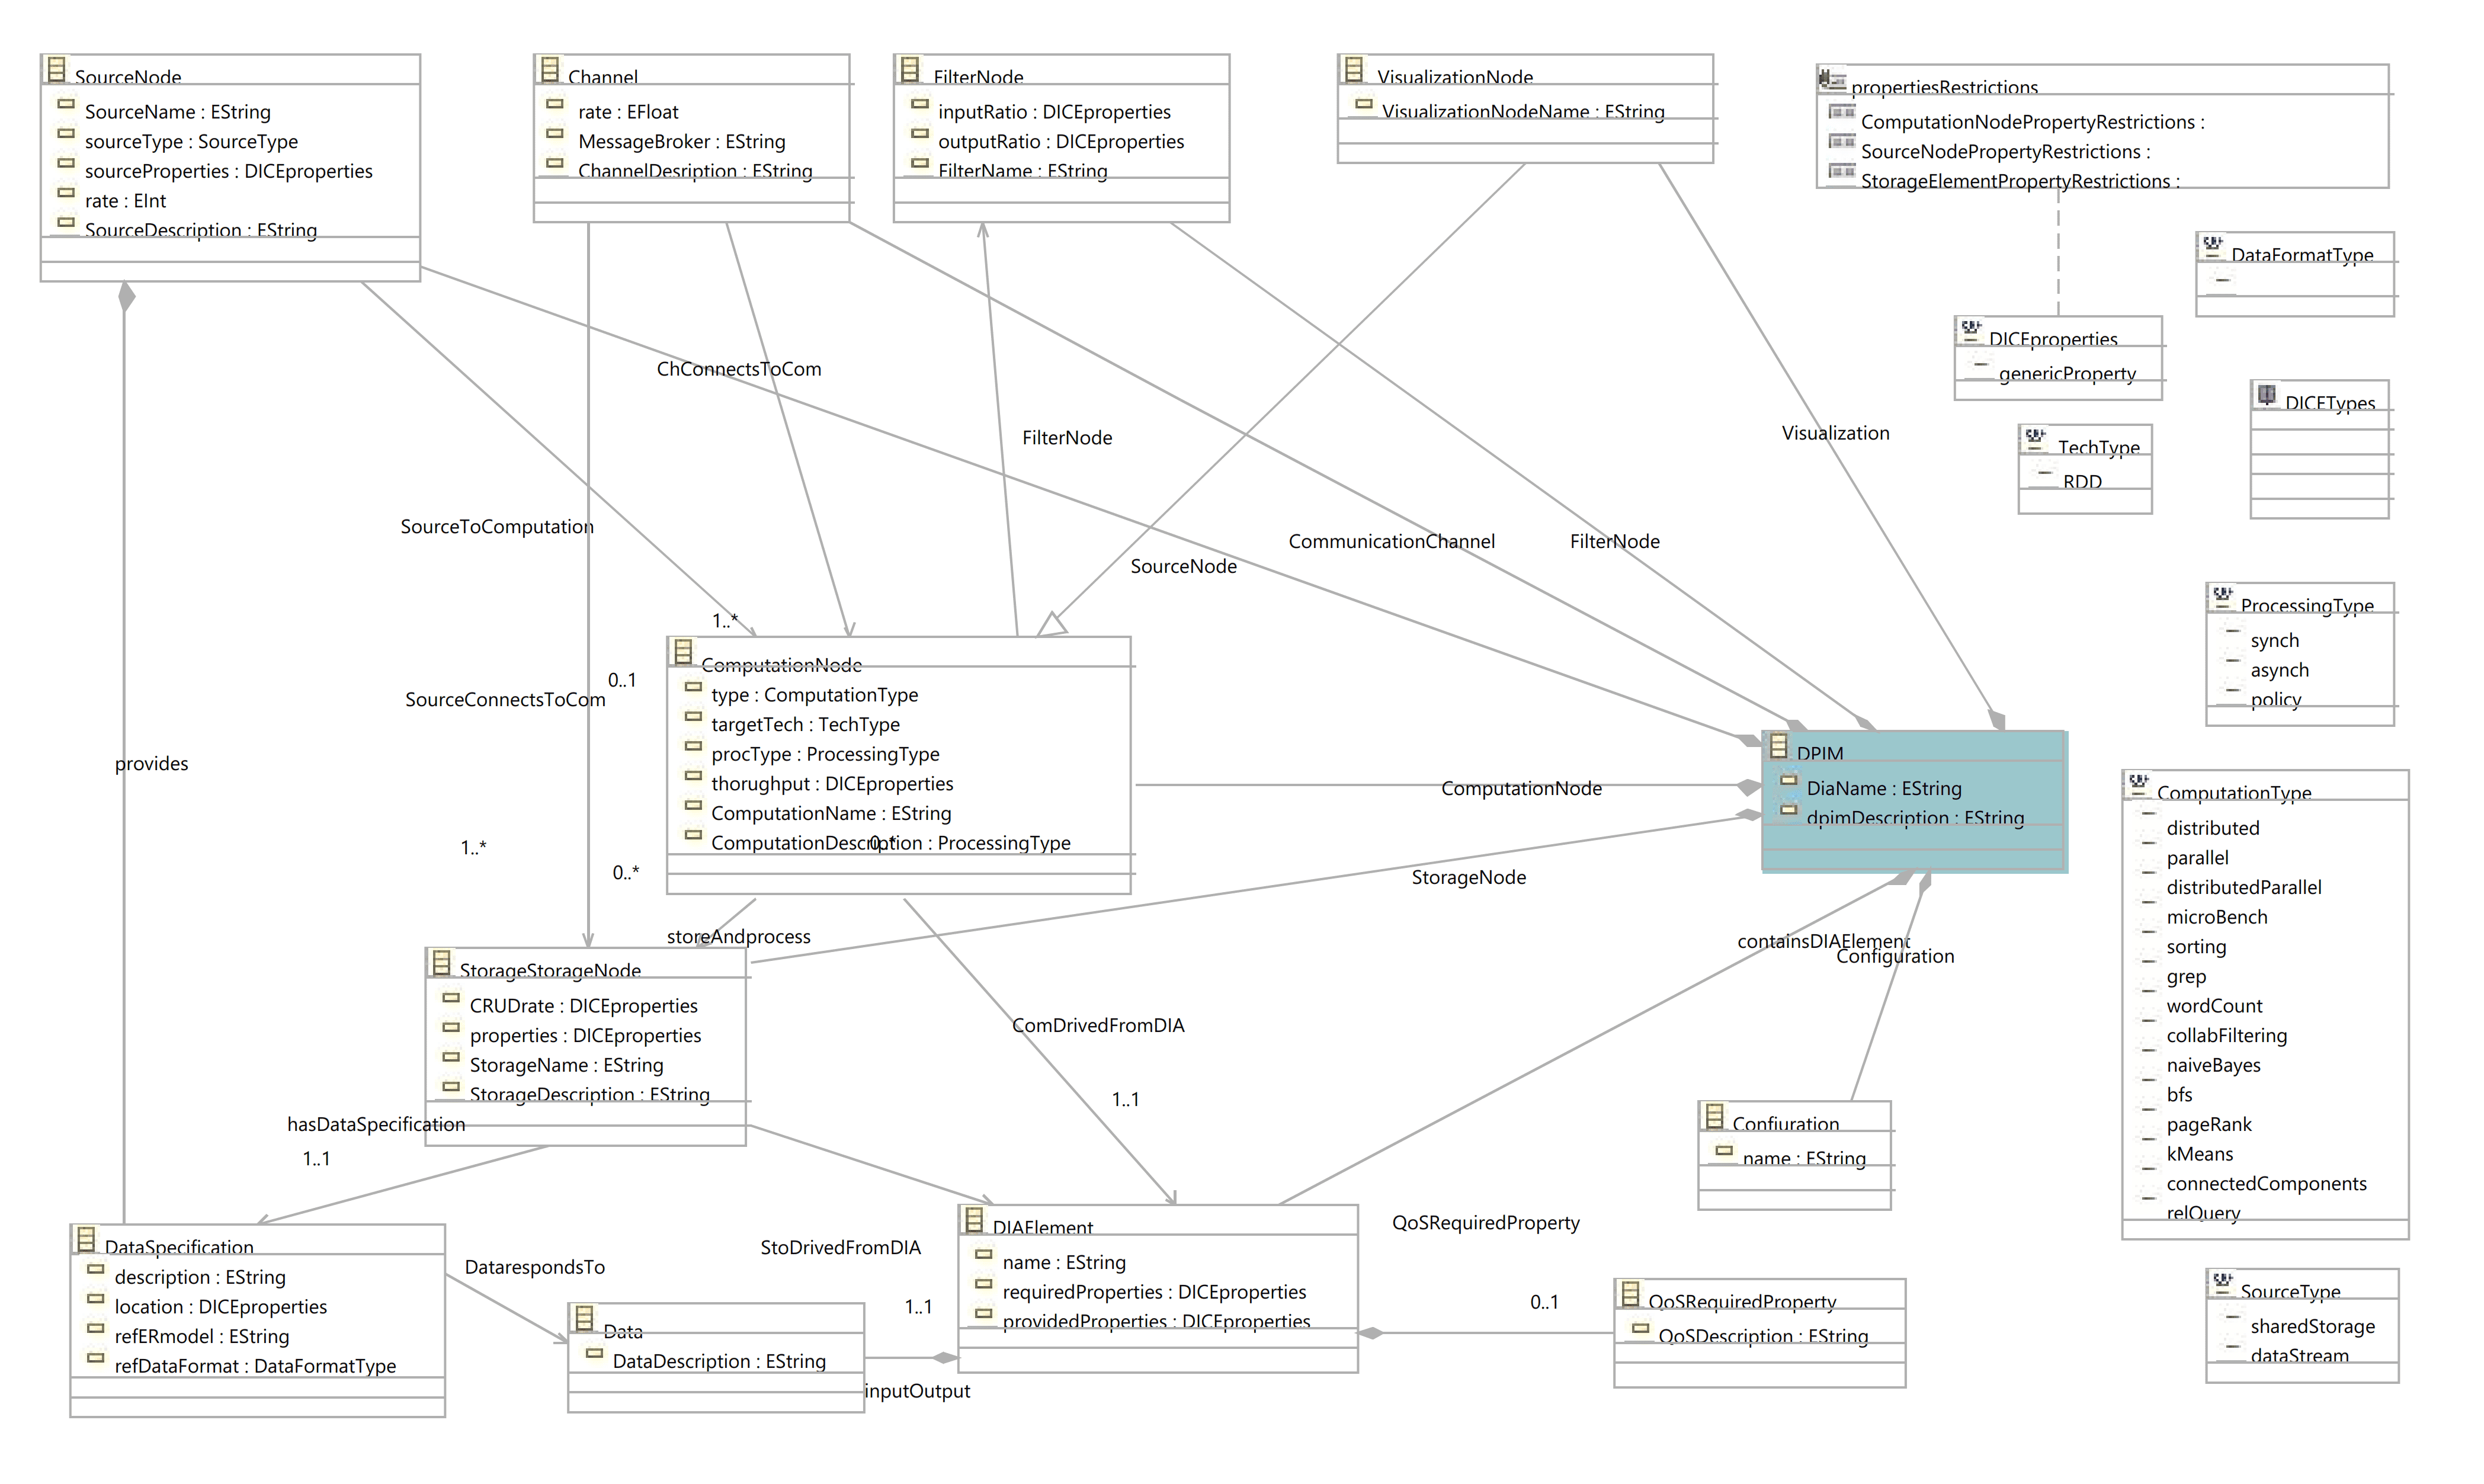
\includegraphics[width=\textwidth]{Images/11.png}
\caption{\label{fig:metamodel}DICE DPIM metamodel.}
\end{sidewaysfigure}

\begin{figure}
\centering
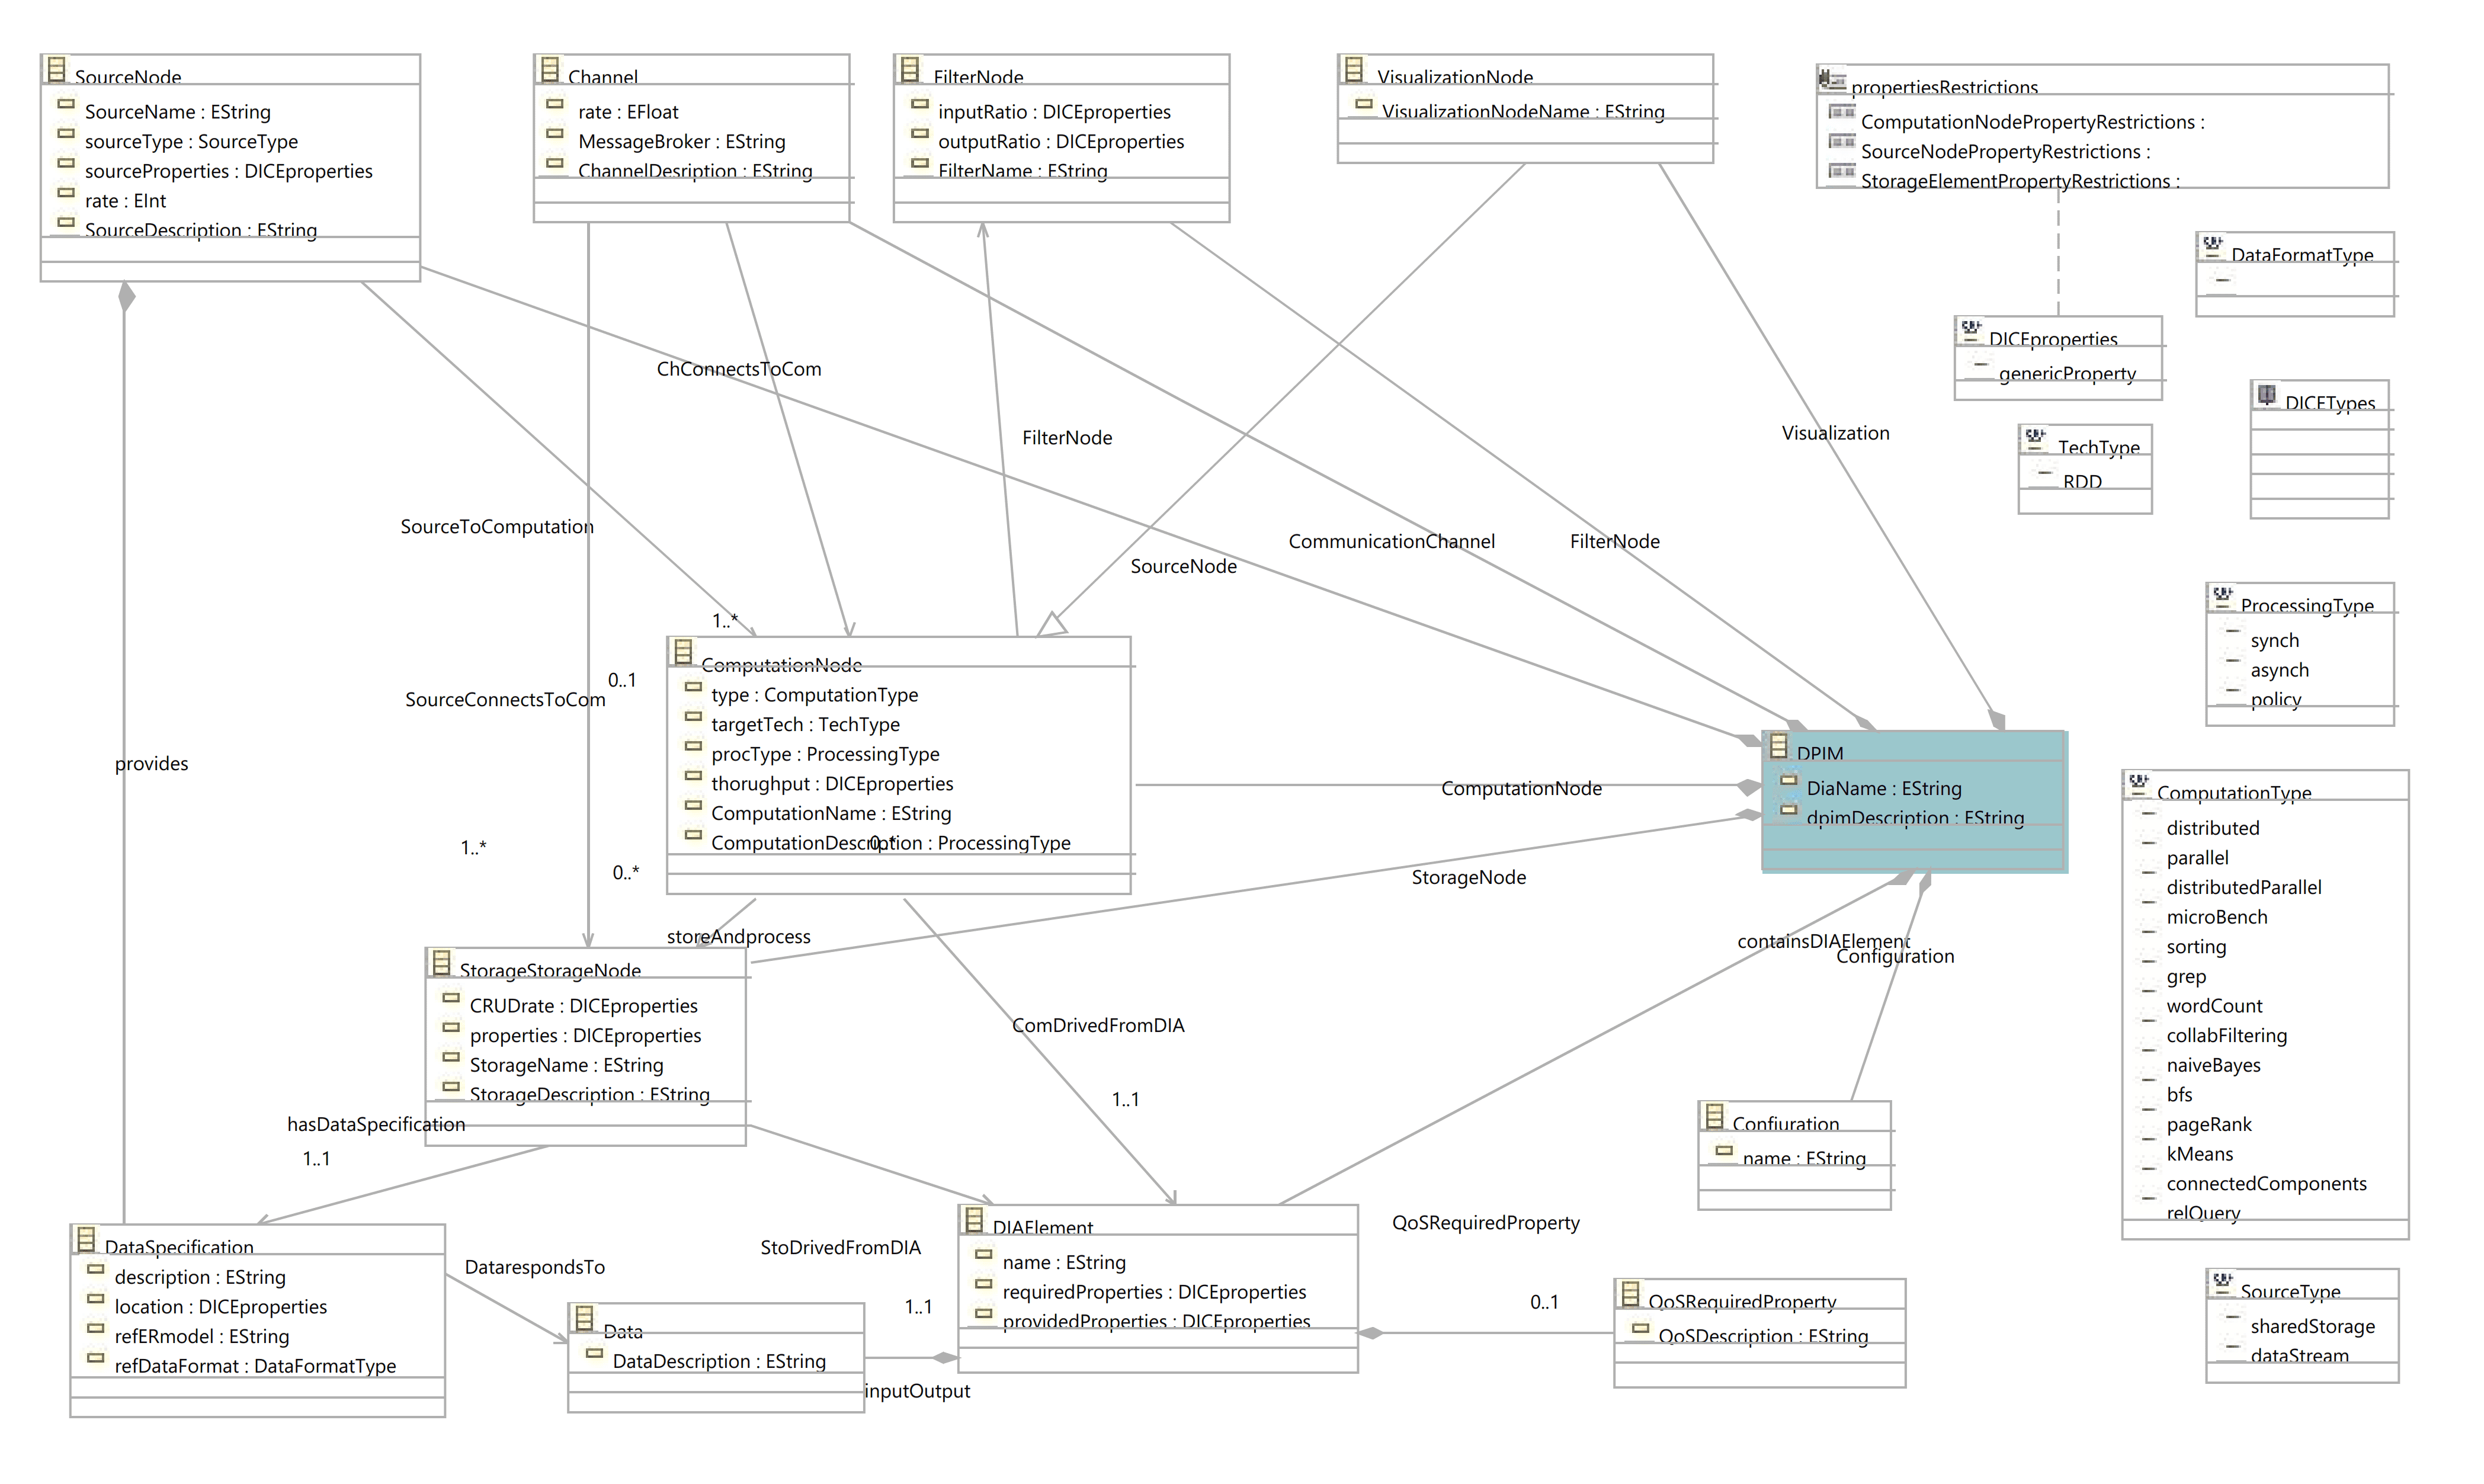
\includegraphics[width=\textwidth]{Images/11.png}
\caption{\label{fig:metamodel2}DICE DPIM metamodel in portrait form.}
\end{figure}

Here is the command to refer to another element (section, figure, table, ...) in the document: \emph{As discussed in Section~\ref{sect:overview} and as shown in Figure~\ref{fig:metamodel}, ...}. Here is how to introduce a bibliographic citation~\cite{DAM}. Bibliographic references should be included in a \texttt{.bib} file. 

Table generation is a bit complicated in Latex. You will soon become proficient, but to start you can rely on tools or external services. See for instance this \href{https://www.tablesgenerator.com}{https://www.tablesgenerator.com}. 


%------------------------------------------------------------------------------------------------------------------------------------------------
\clearpage
{\color{Blue}{\section{Specific Requirements}}}
\label{sect:requirements}
\subsection{External Interface Requirements}

\subsubsection{User Interfaces}
% In this section we present user interfaces for Students and Educators. 
% \begin{center}
%     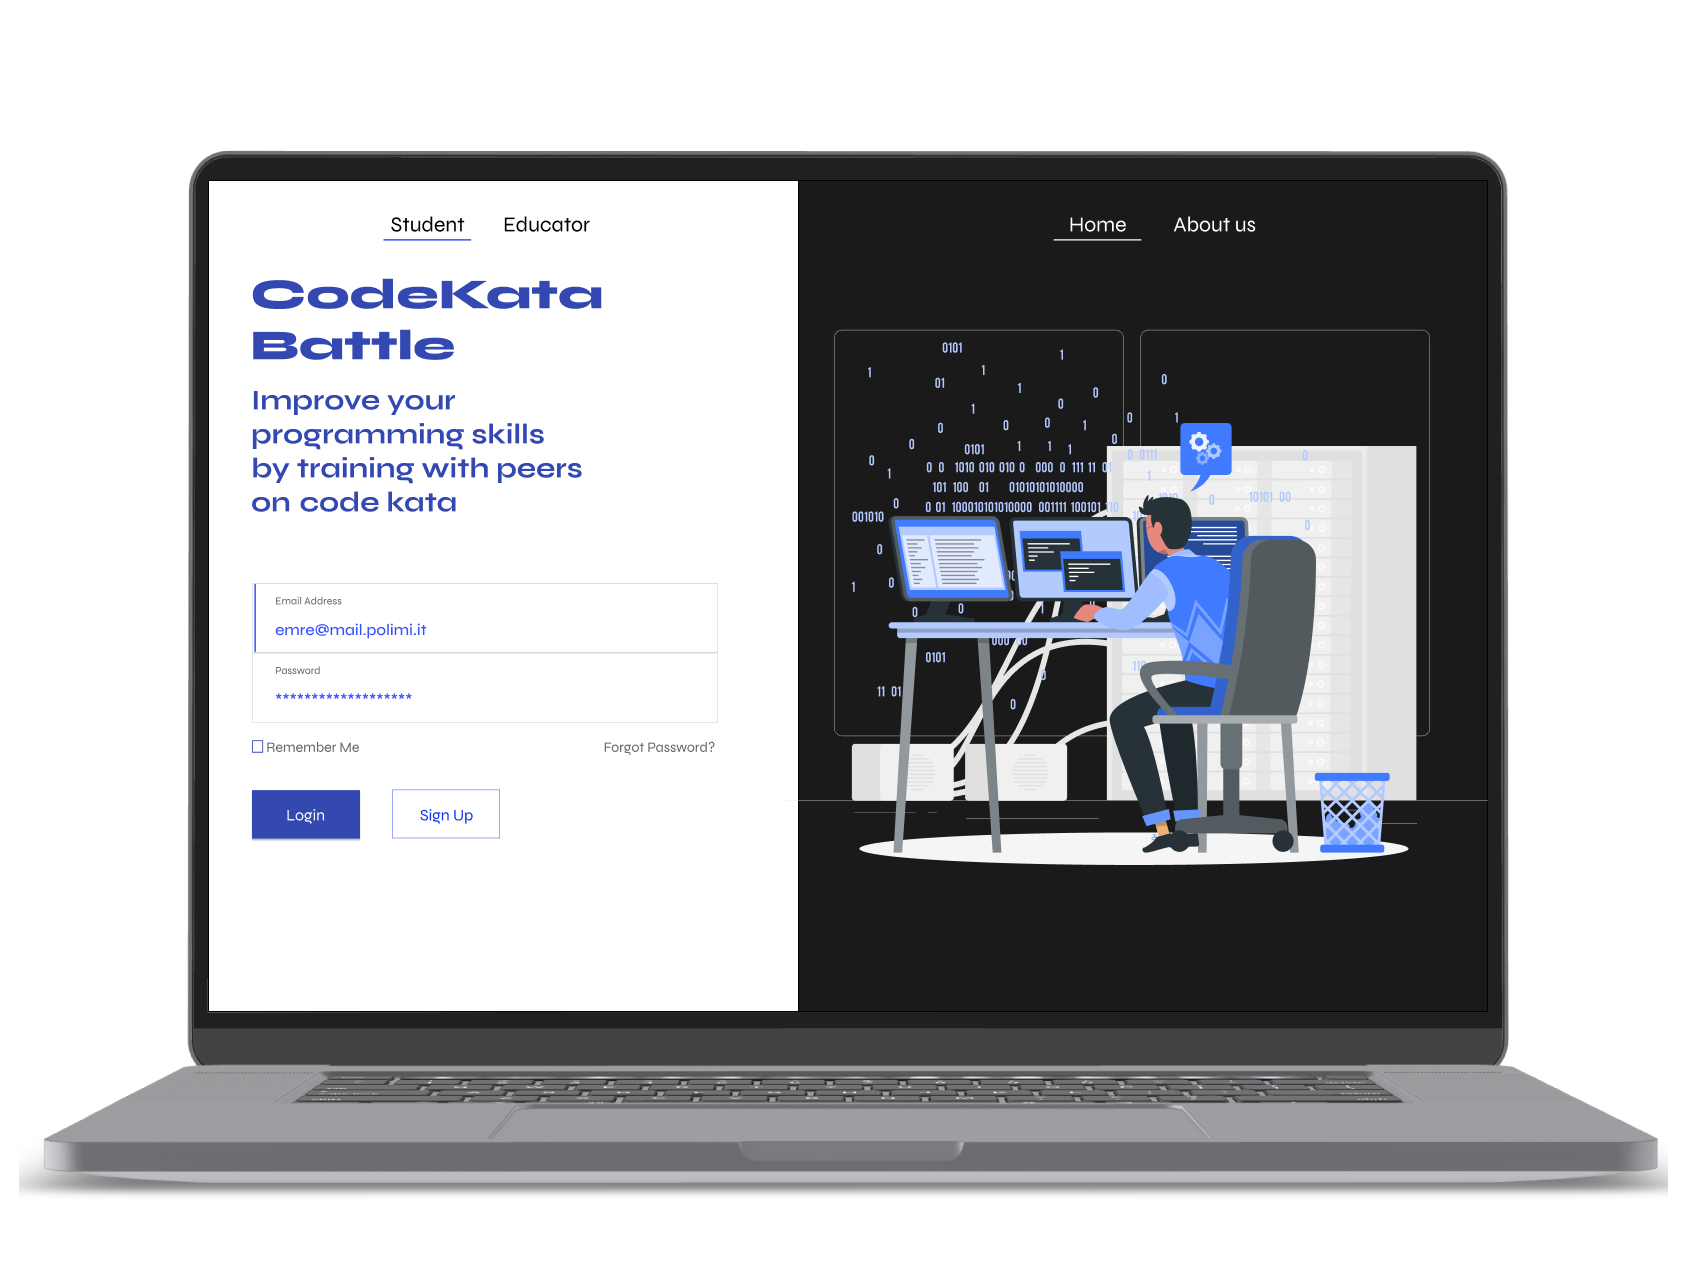
\includegraphics[scale=0.13]{Images/ui-ux/login-signup/student_login.png}
%     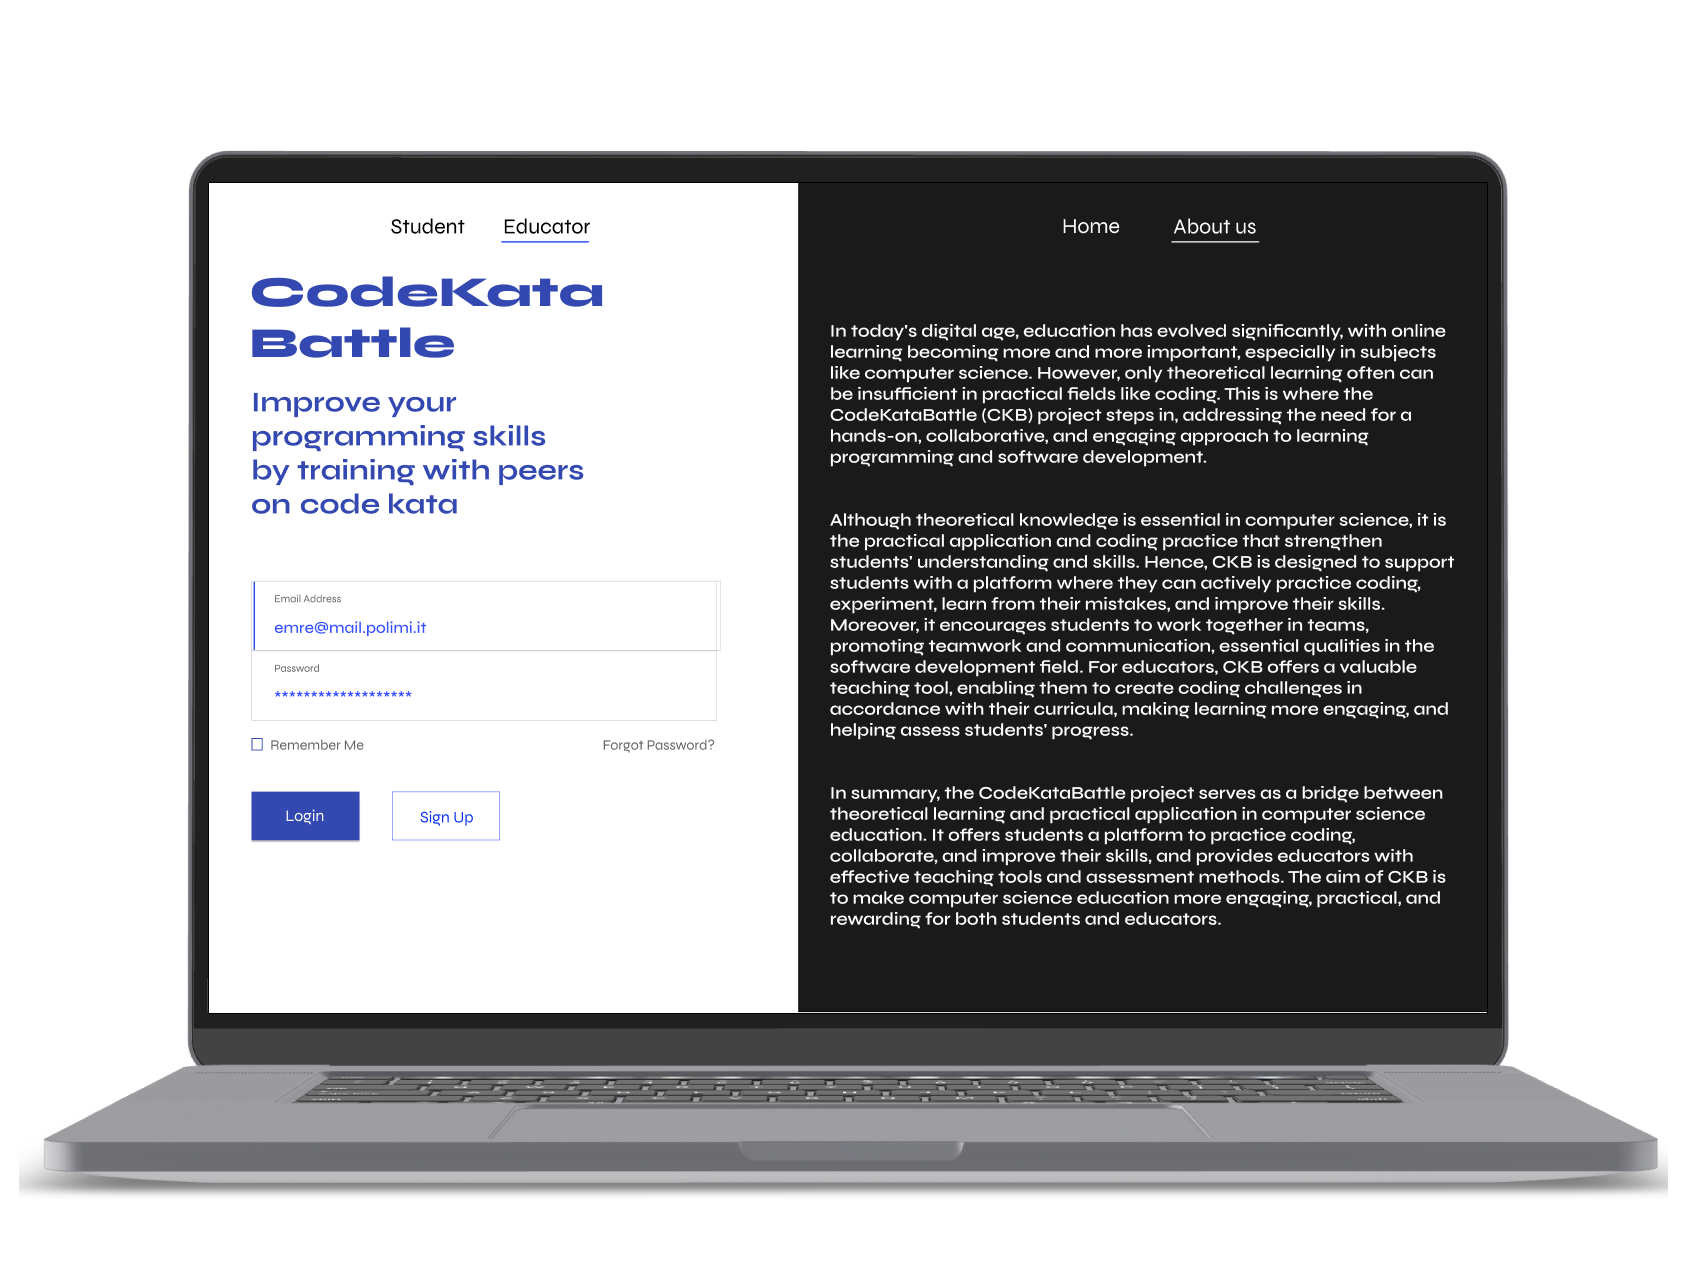
\includegraphics[scale=0.13]{Images/ui-ux/login-signup/educator_login.png}
% \end{center}
%     \begin{center}
%         (a) Login Screens
%     \end{center}
% \begin{center}
%     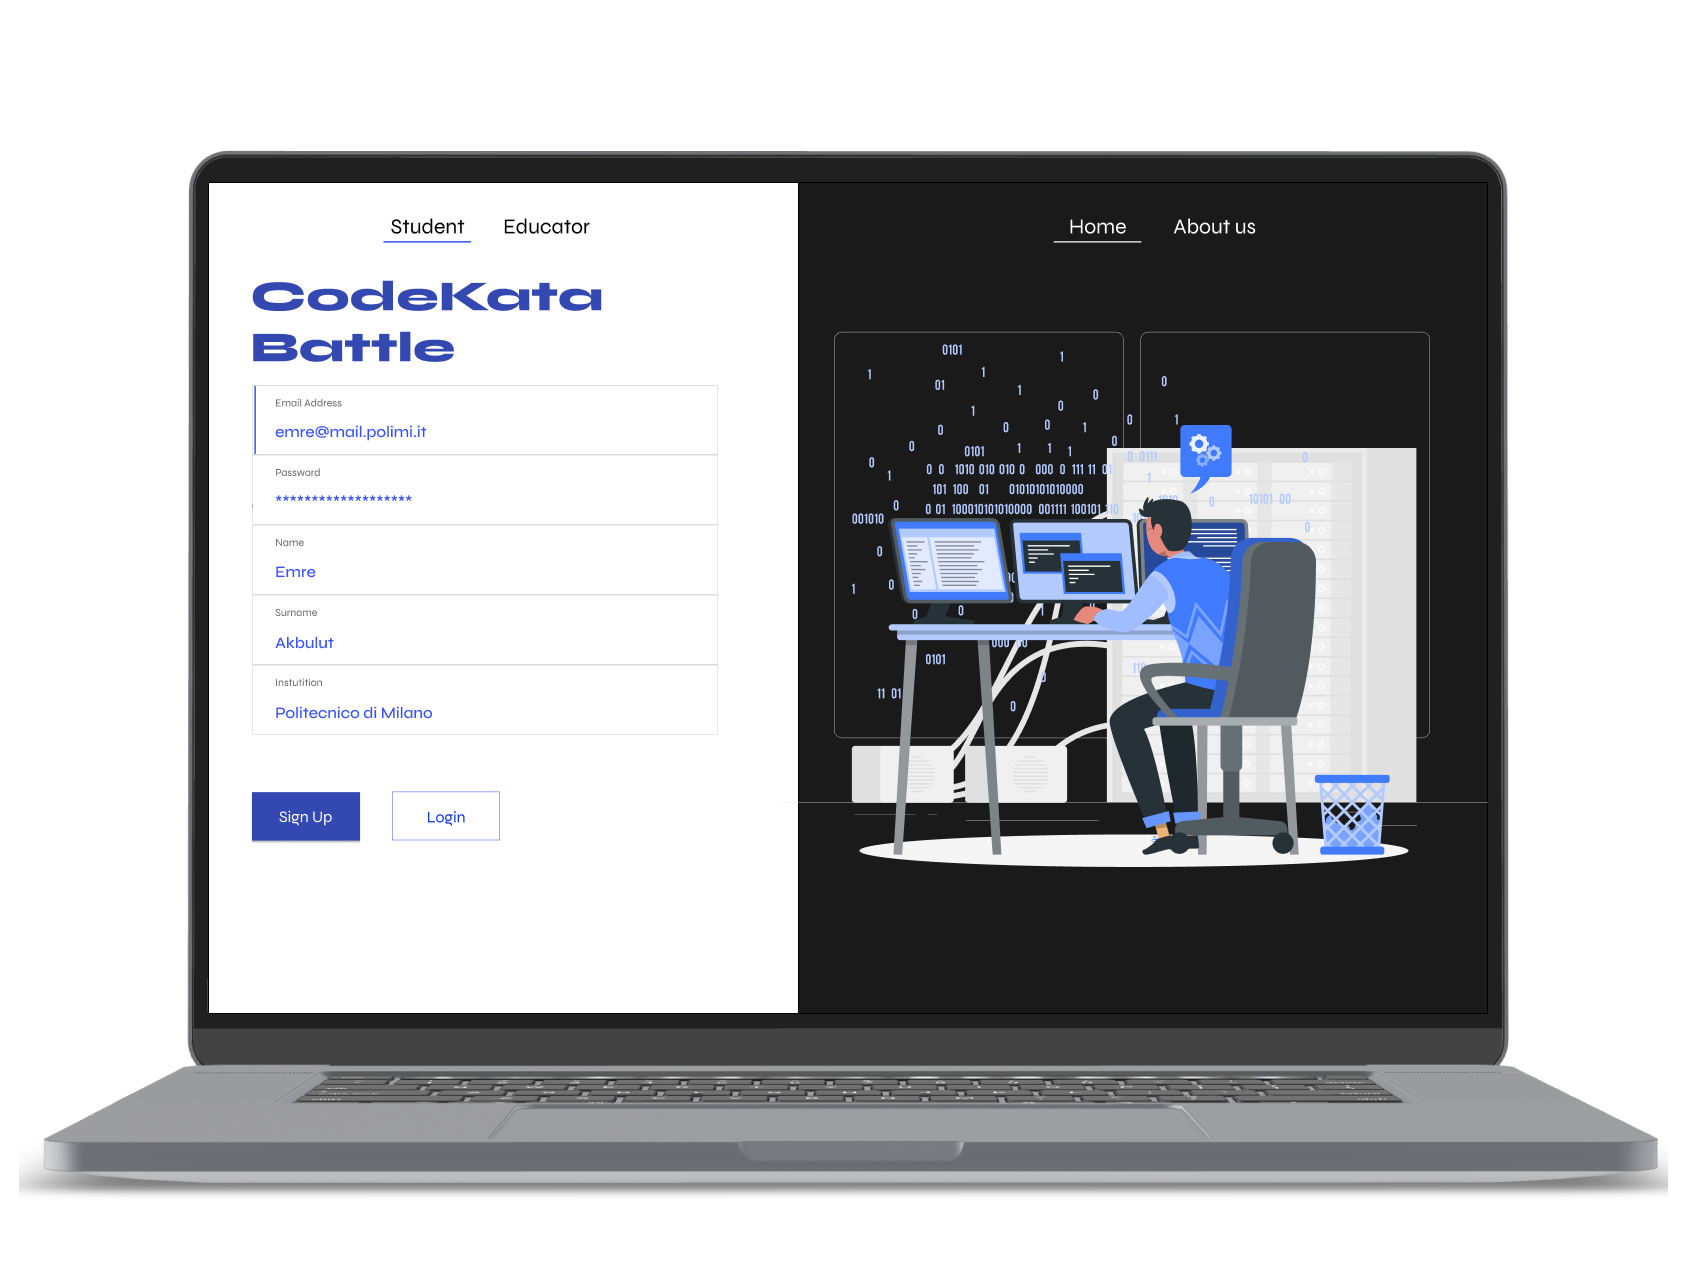
\includegraphics[scale=0.13]{Images/ui-ux/login-signup/student_signup.png}
%     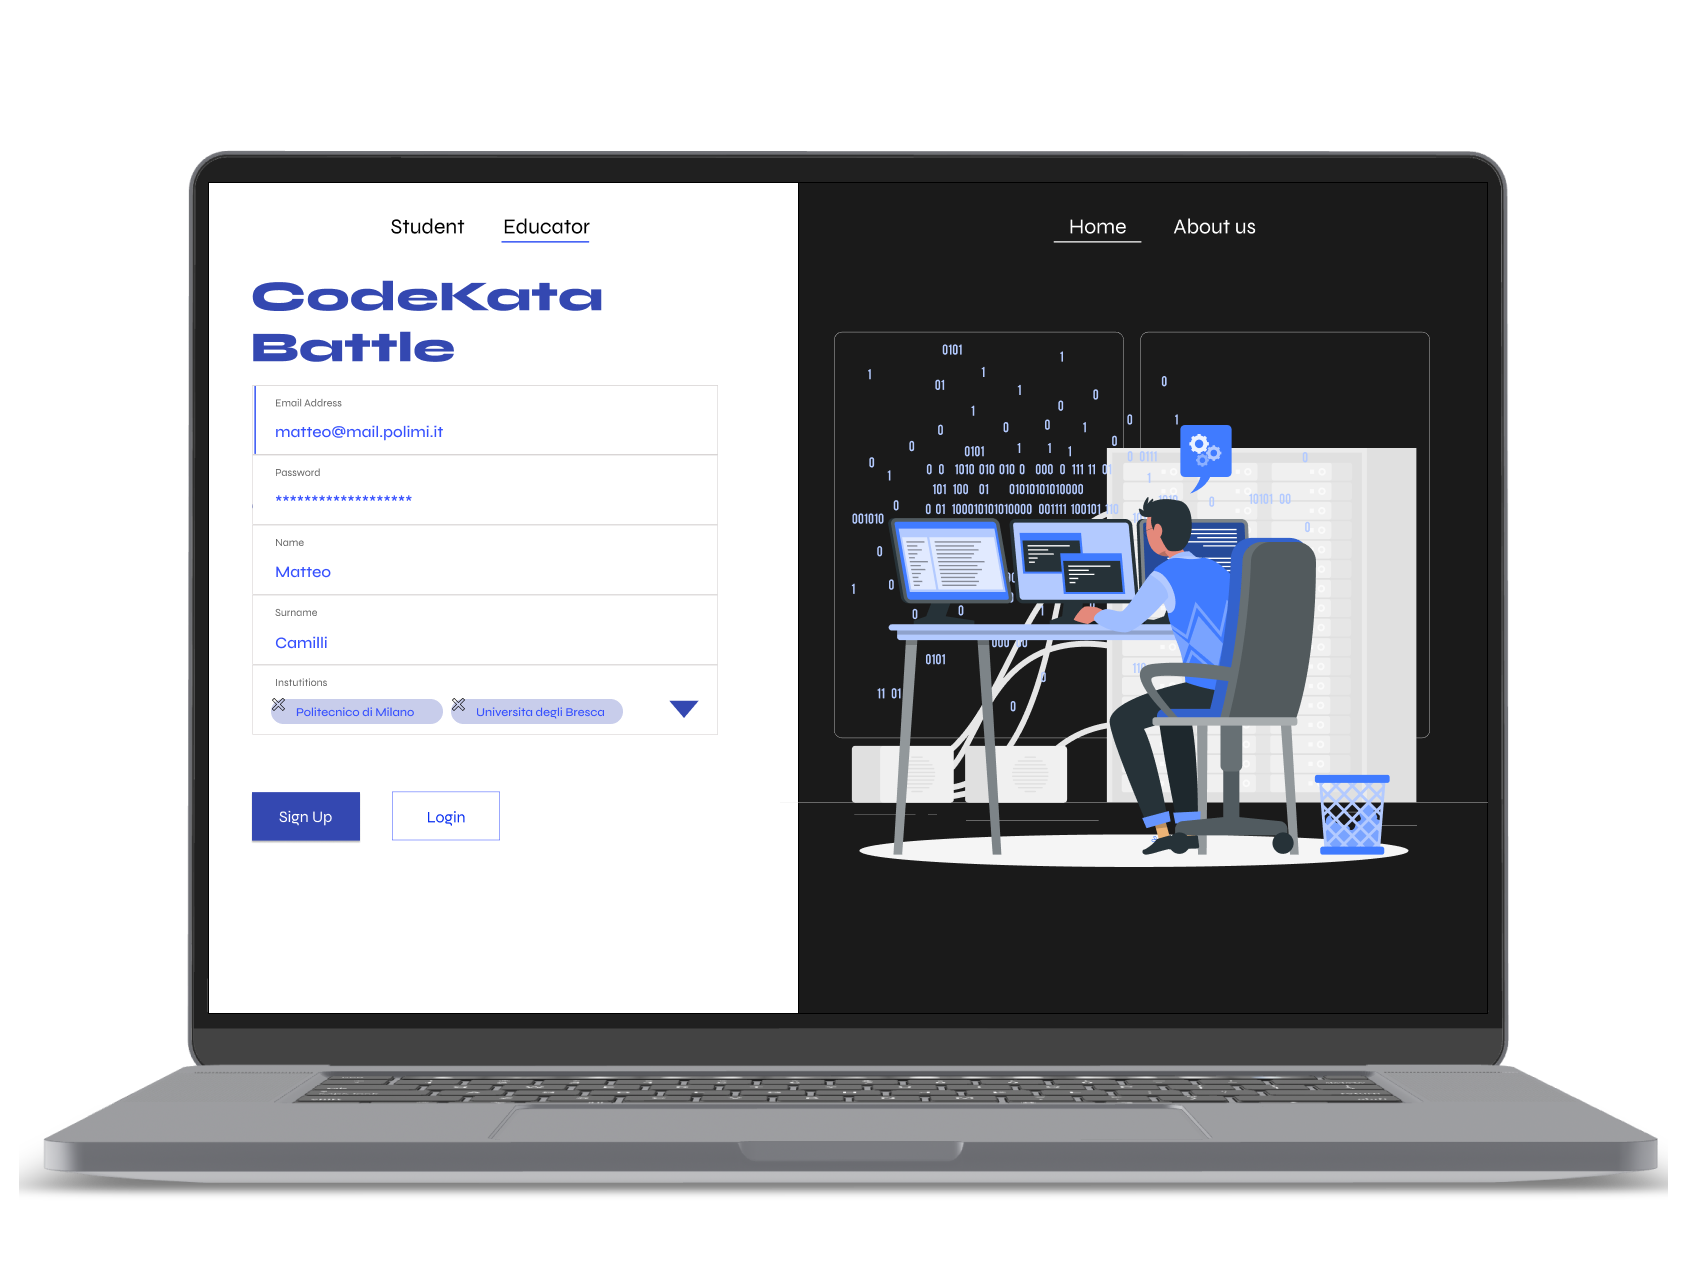
\includegraphics[scale=0.13]{Images/ui-ux/login-signup/educator_signup.png}
%     (a) Sign up Screens
% \end{center}
% \newpage
% \begin{center}
%     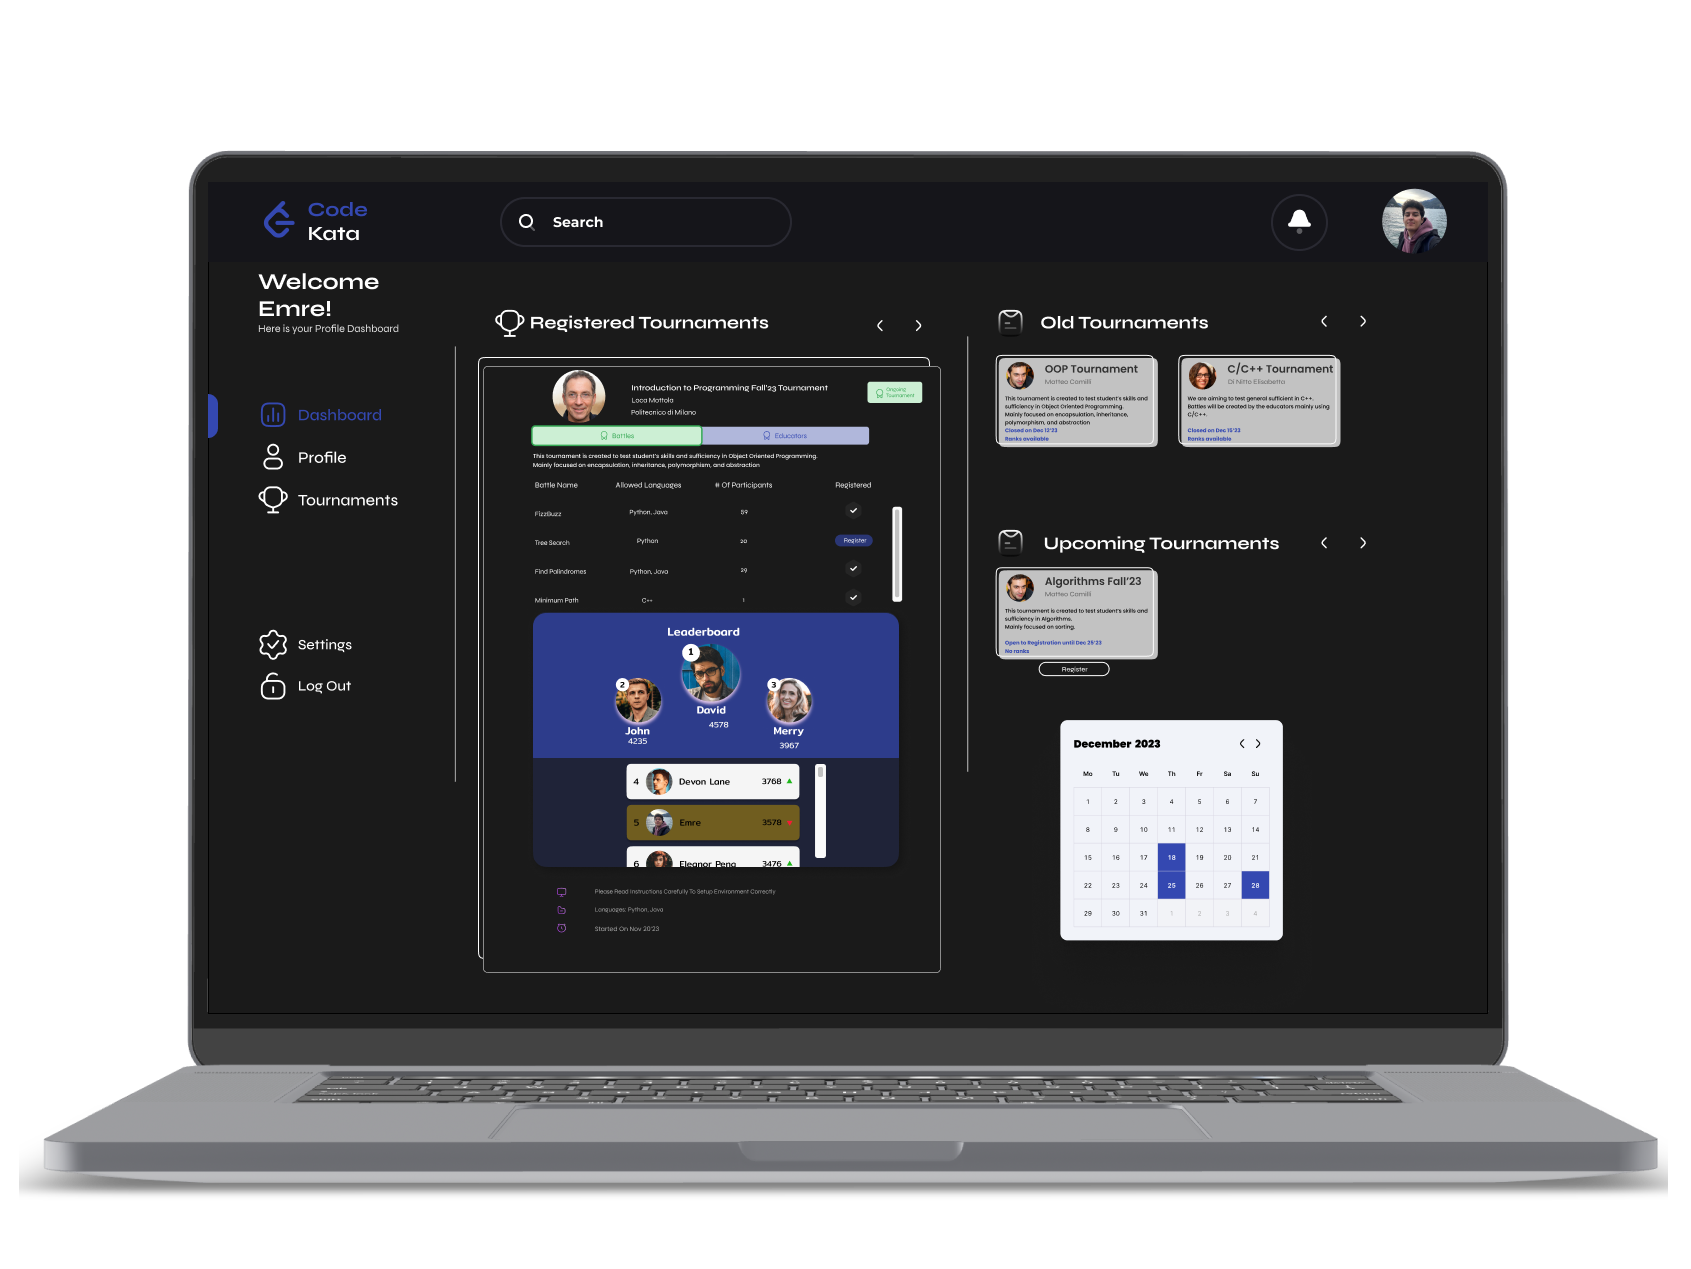
\includegraphics[scale=0.13]{Images/ui-ux/student_dashboard/student_dashboard_1.png}
%     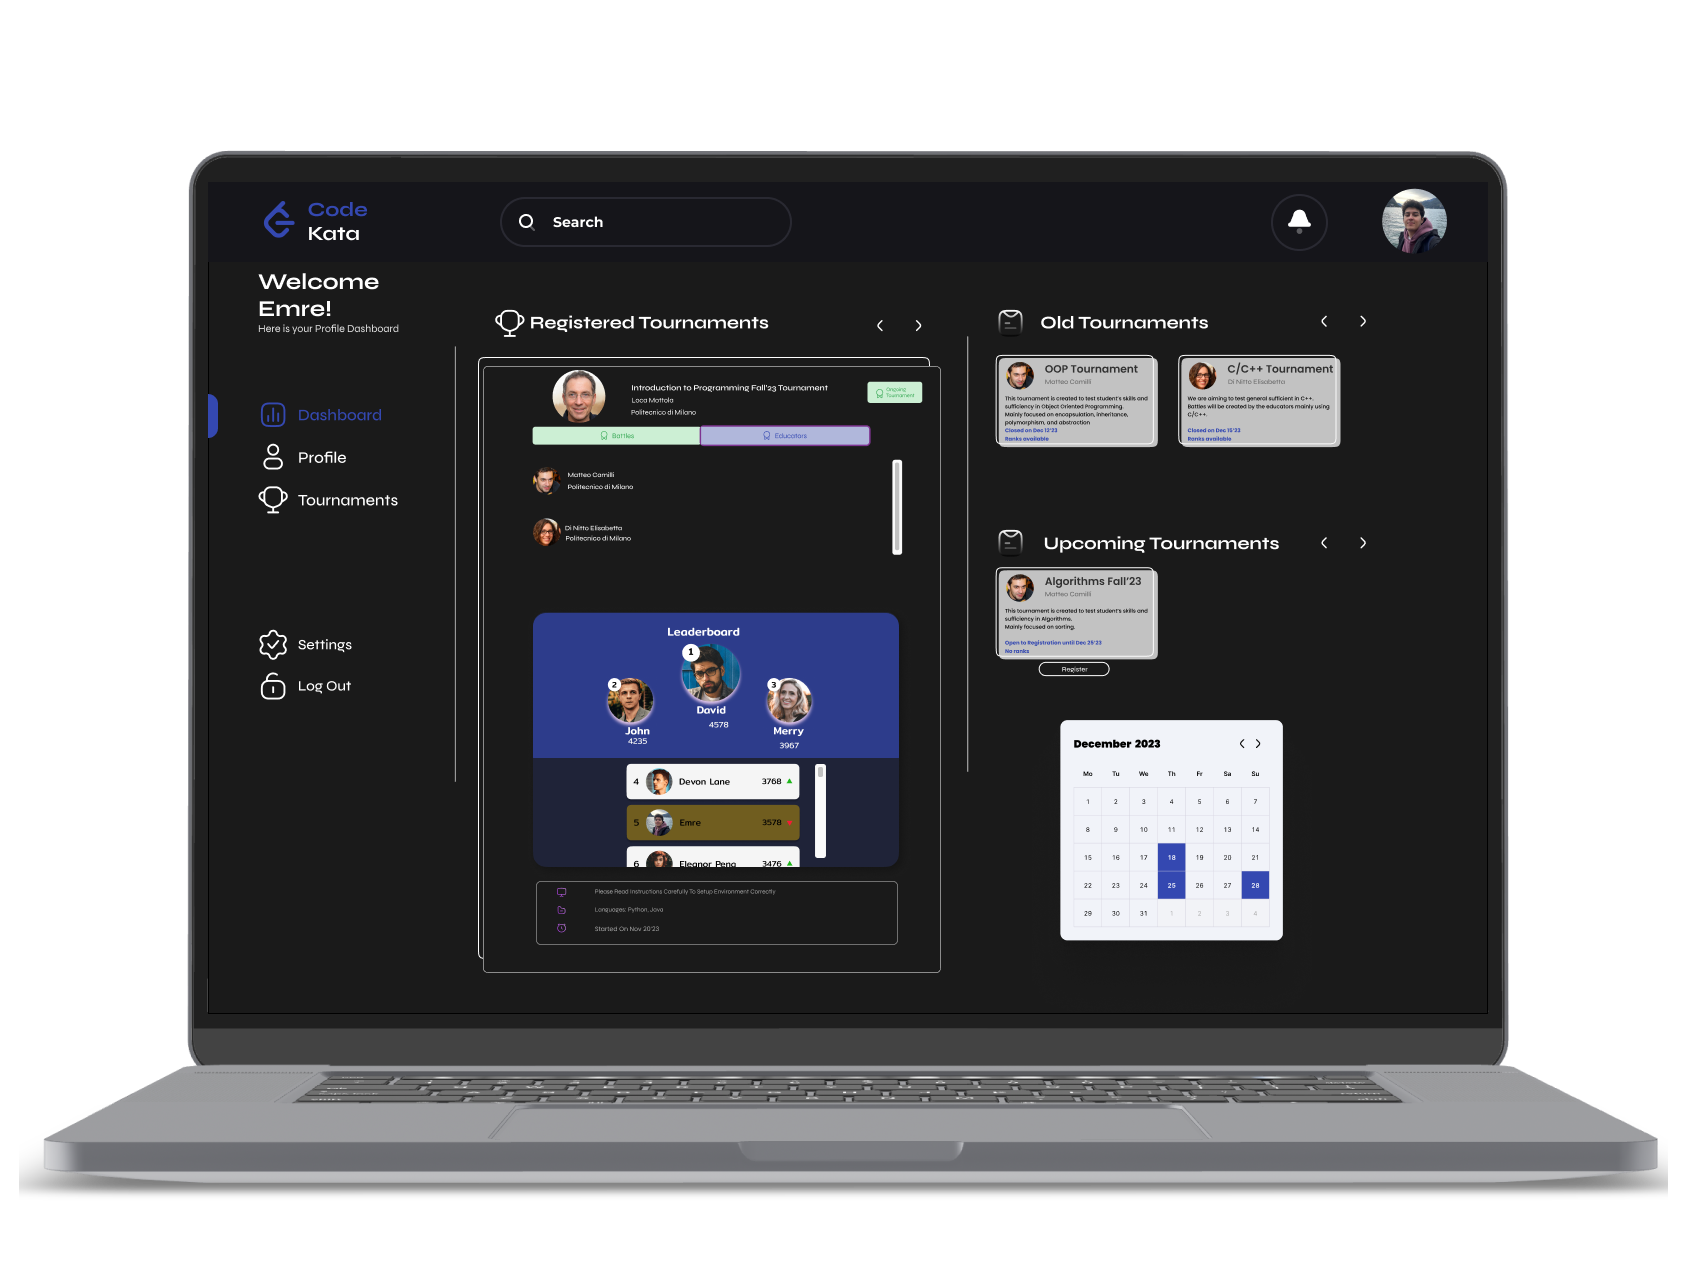
\includegraphics[scale=0.13]{Images/ui-ux/student_dashboard/student_dashboard_2.png}
%             (a) Student Dashboard
% \end{center}
% \begin{center}
%     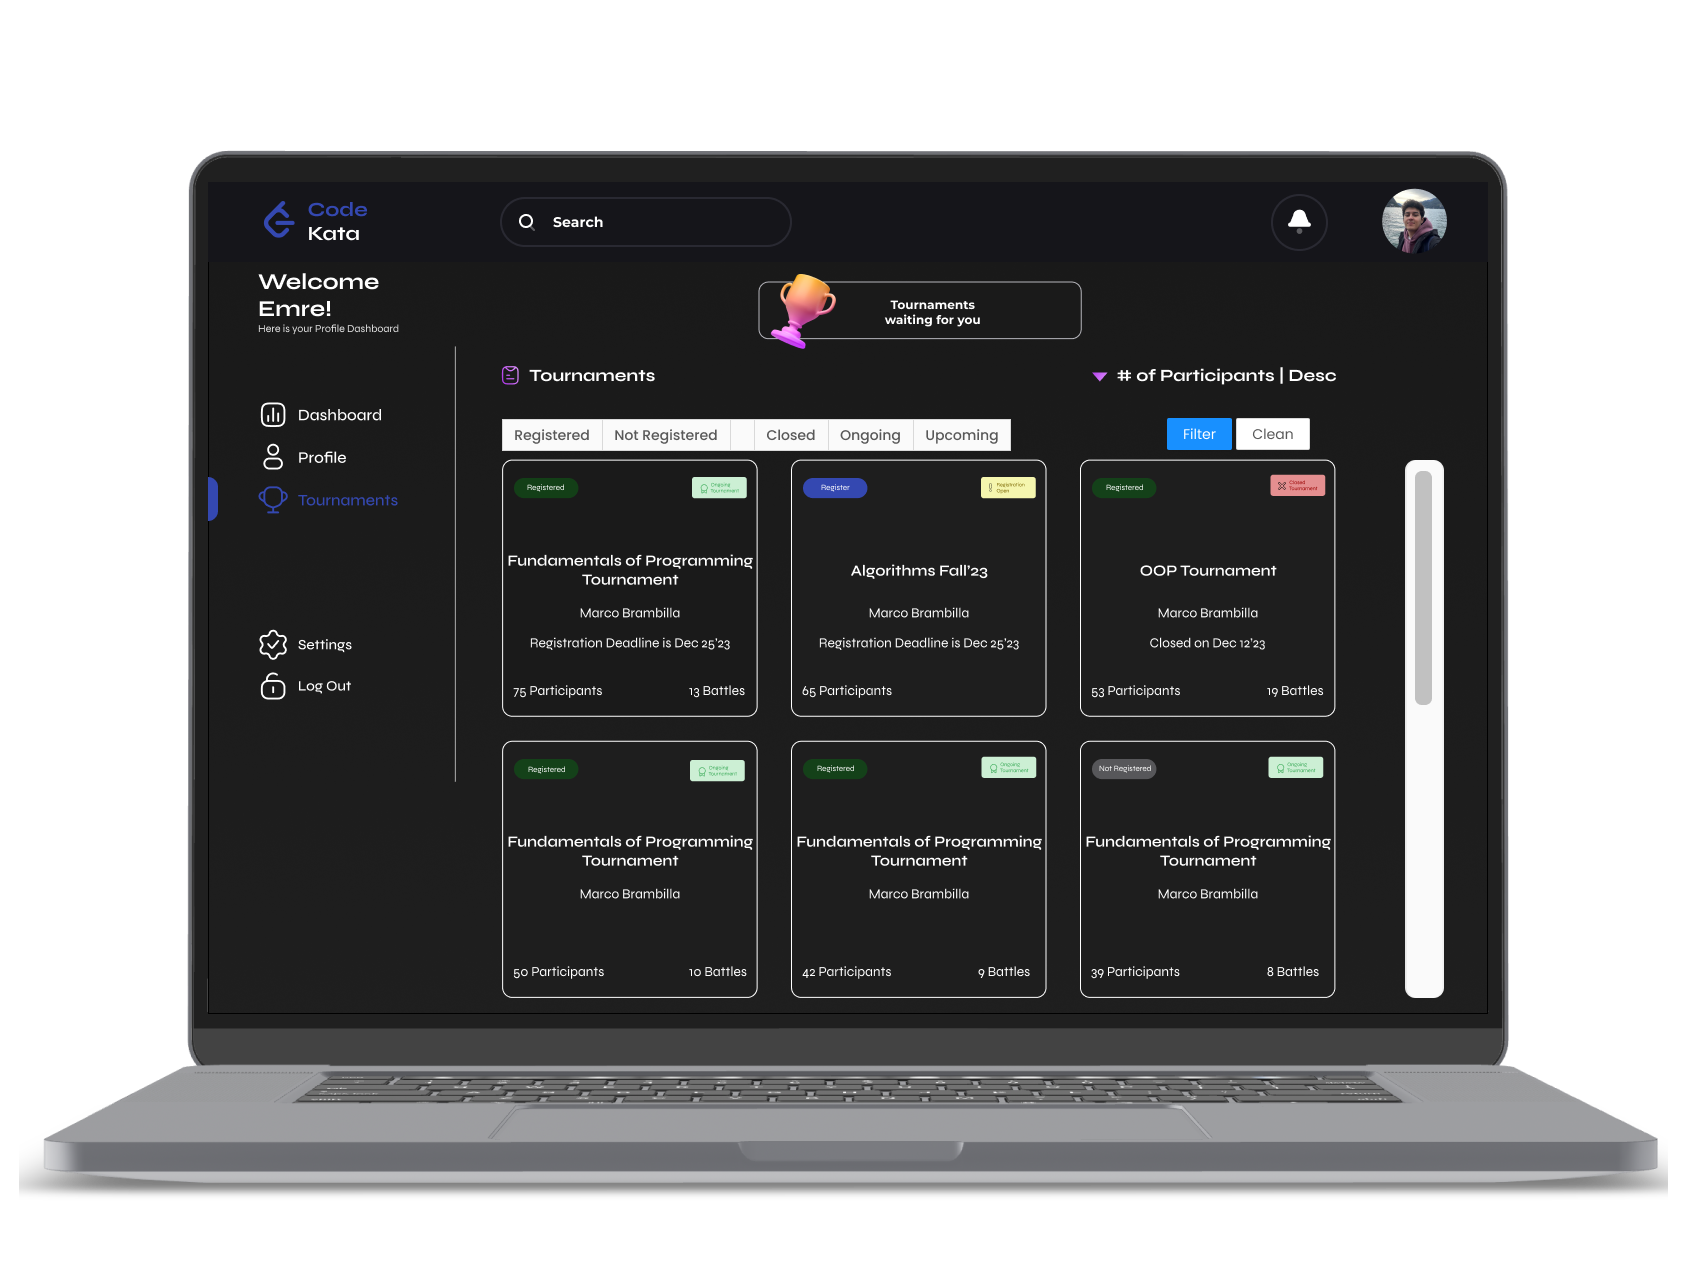
\includegraphics[scale=0.13]{Images/ui-ux/student_tournaments/student_tournaments_1.png}
%     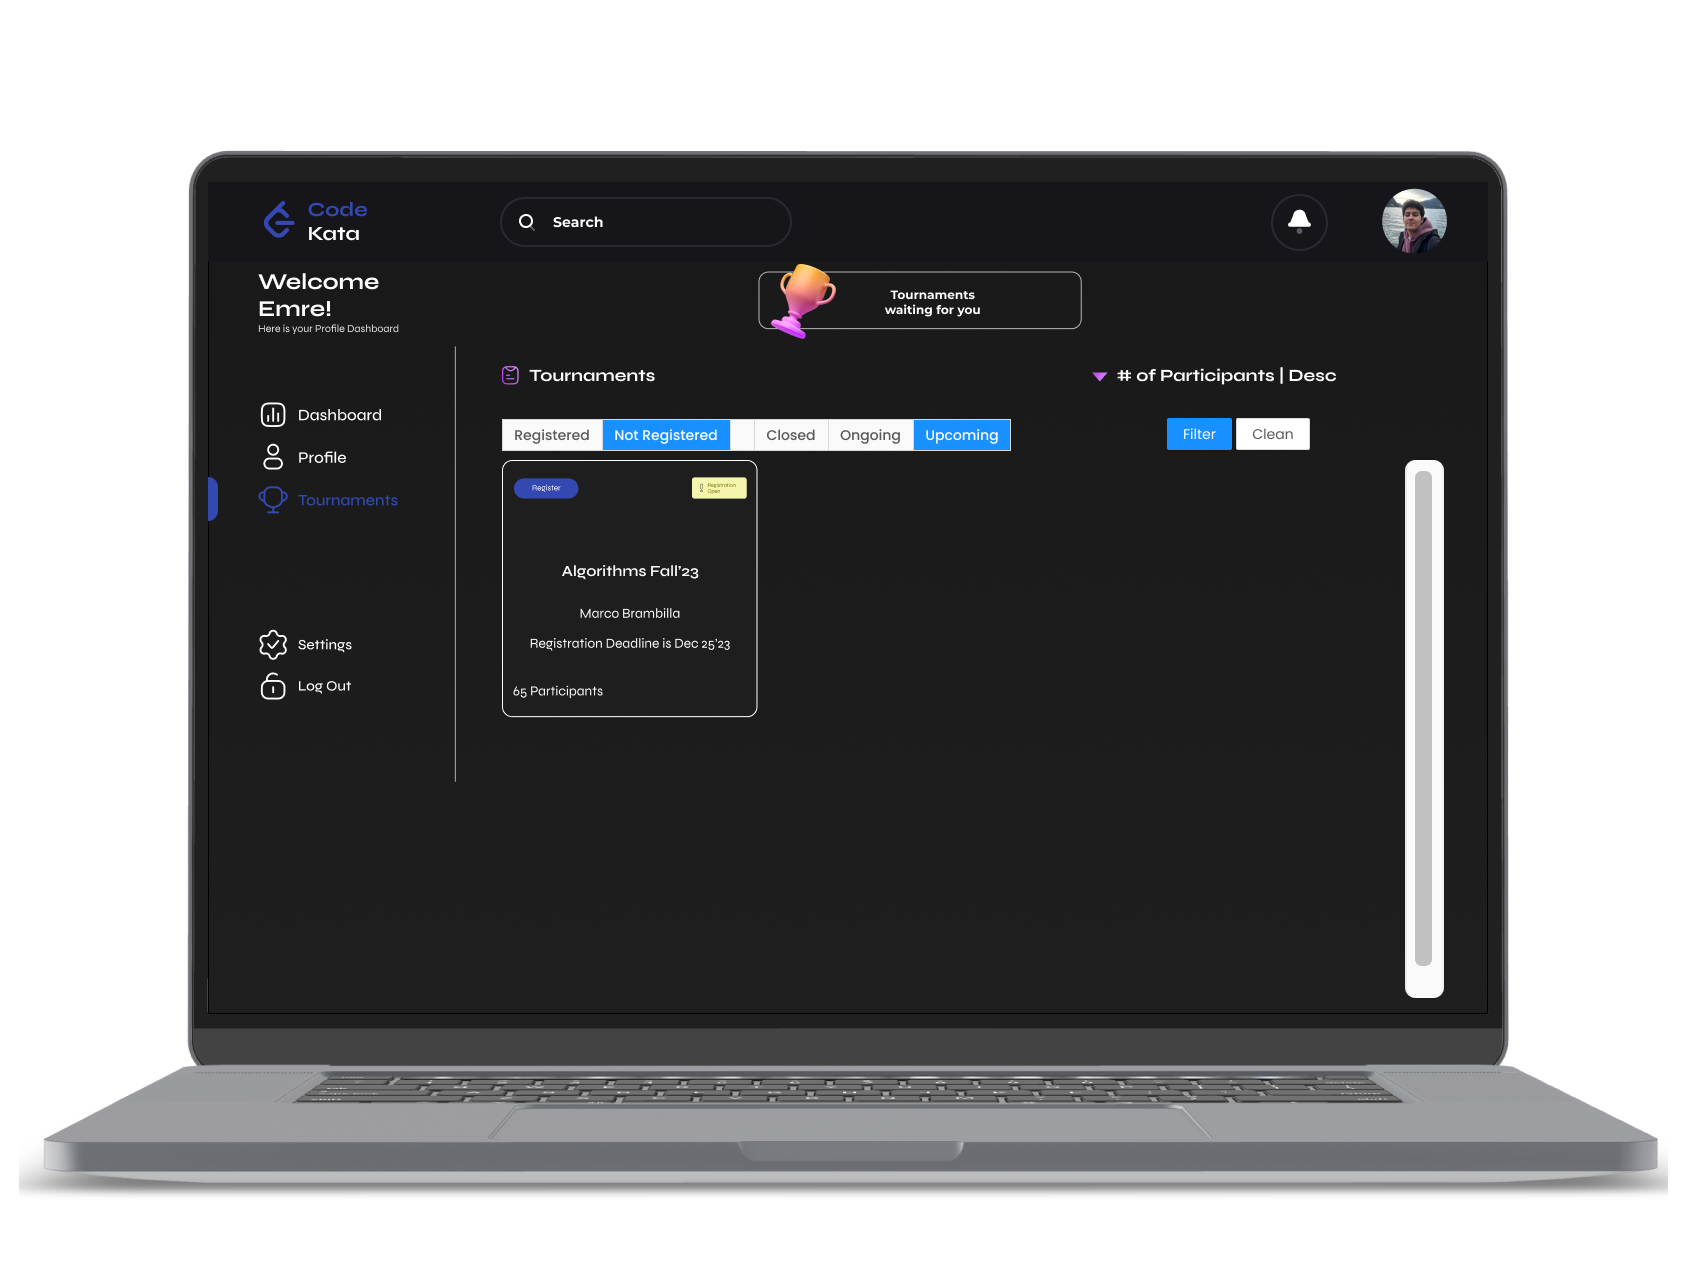
\includegraphics[scale=0.13]{Images/ui-ux/student_tournaments/student_tournaments_2.png}    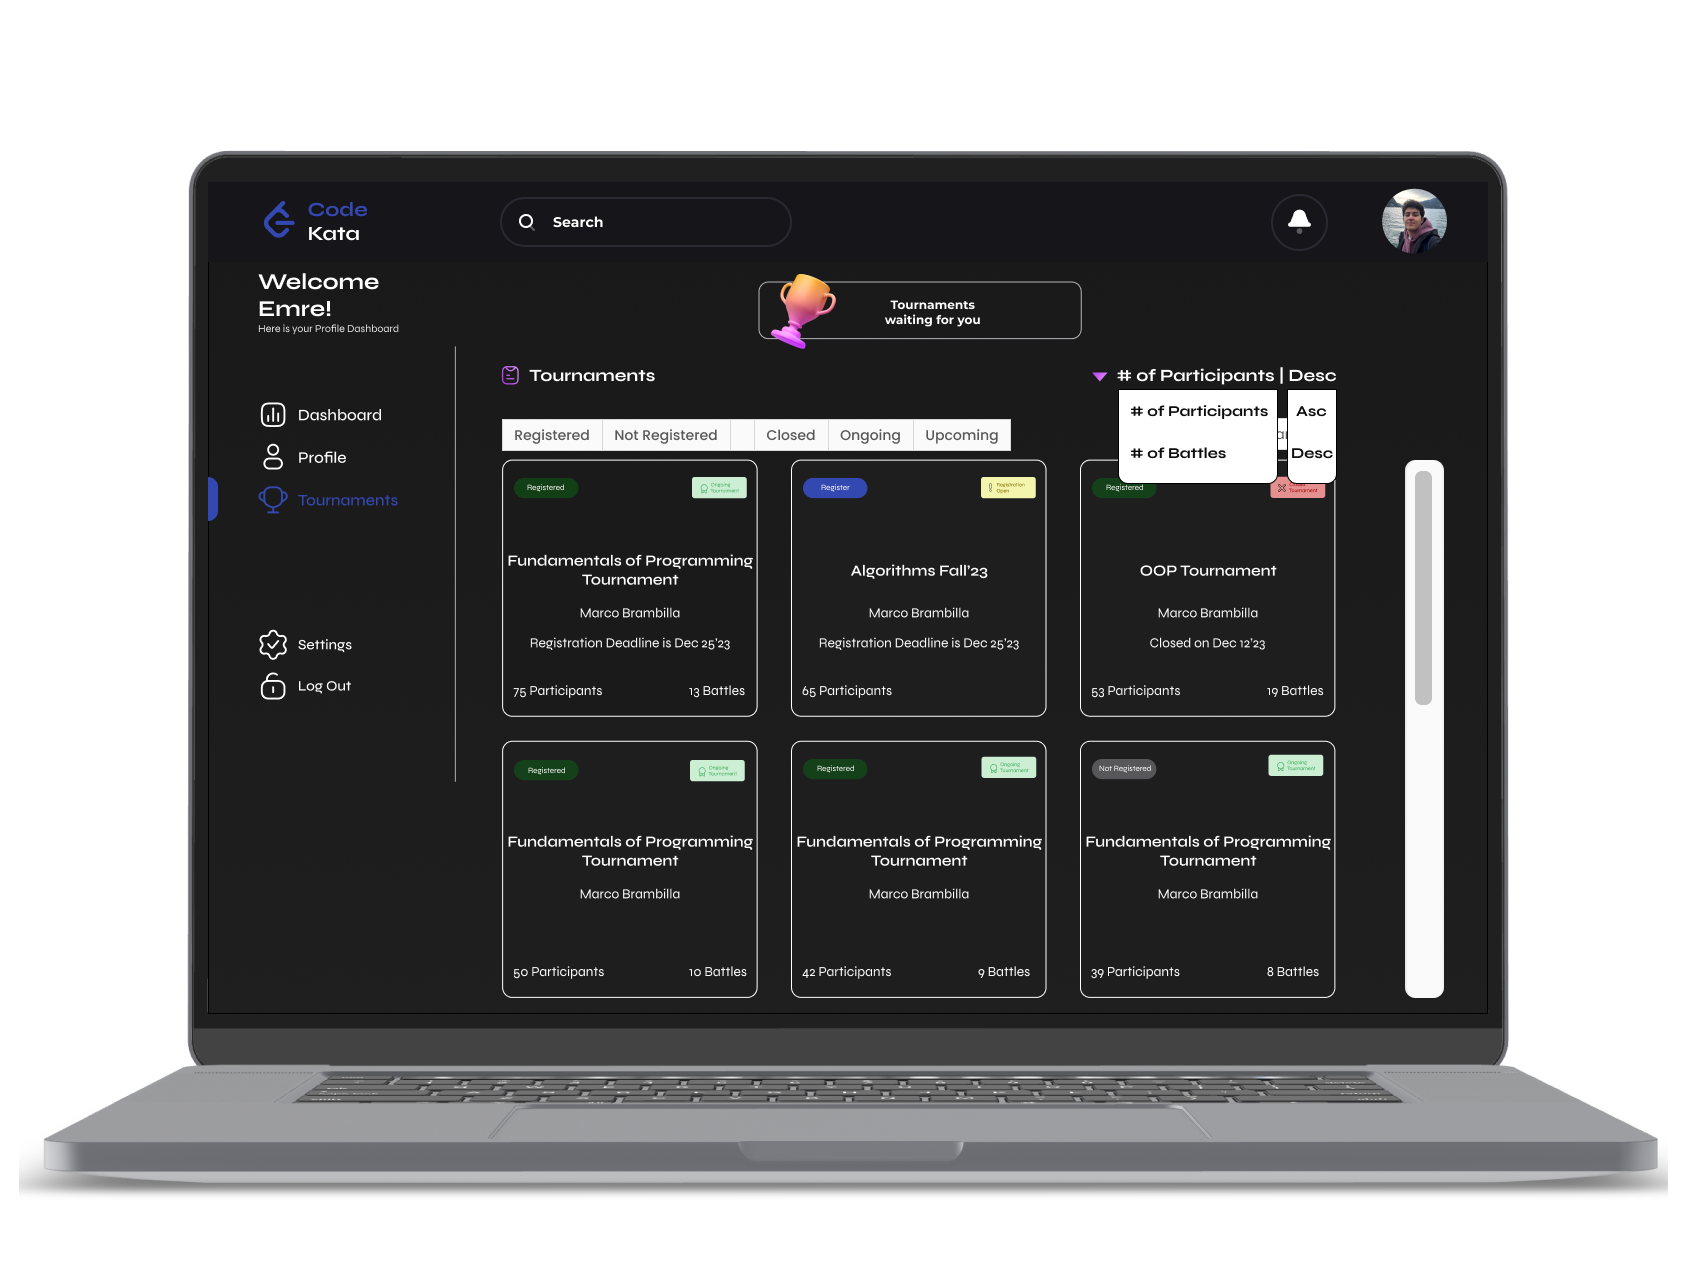
\includegraphics[scale=0.13]{Images/ui-ux/student_tournaments/student_tournaments_3.png}    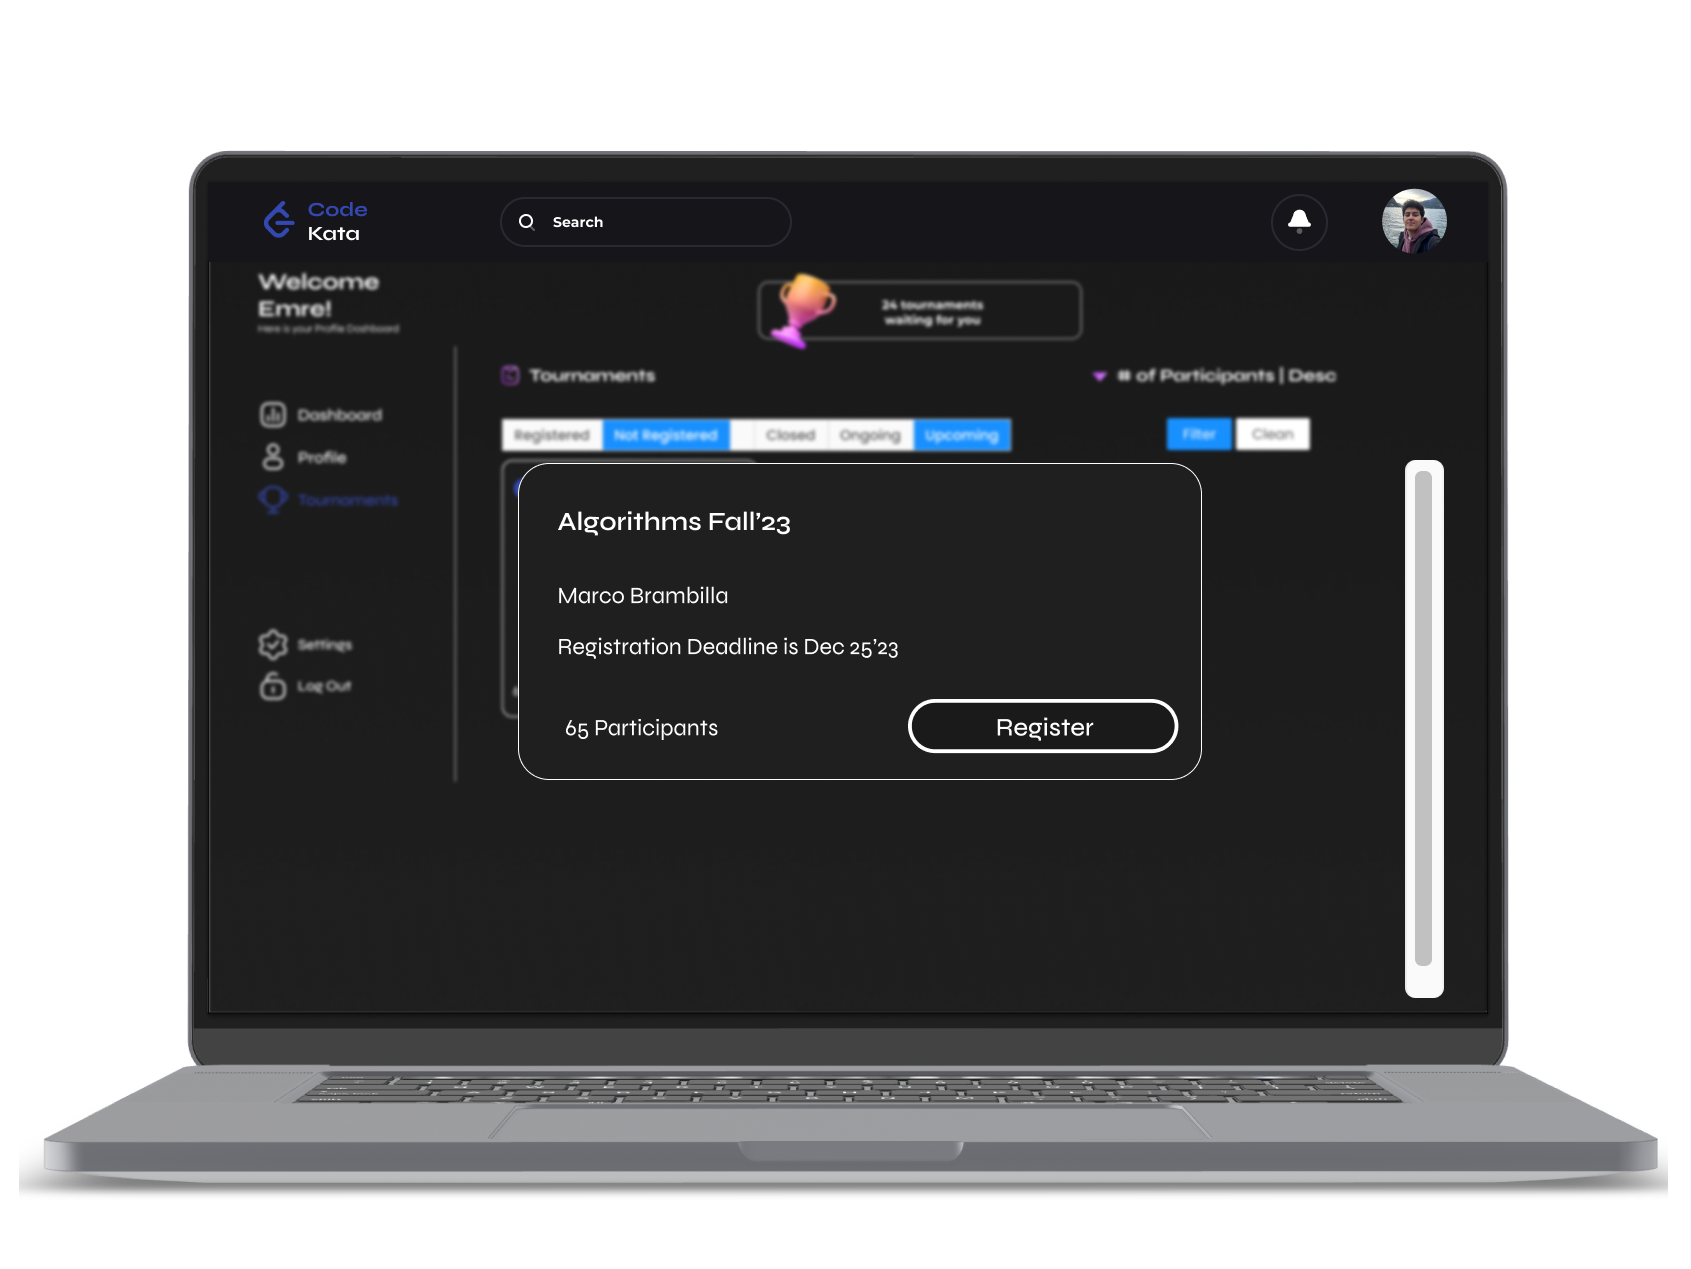
\includegraphics[scale=0.13]{Images/ui-ux/student_tournaments/student_tournaments_4.png}
%         (a) Student Tournaments
% \end{center}

% \begin{center}
%     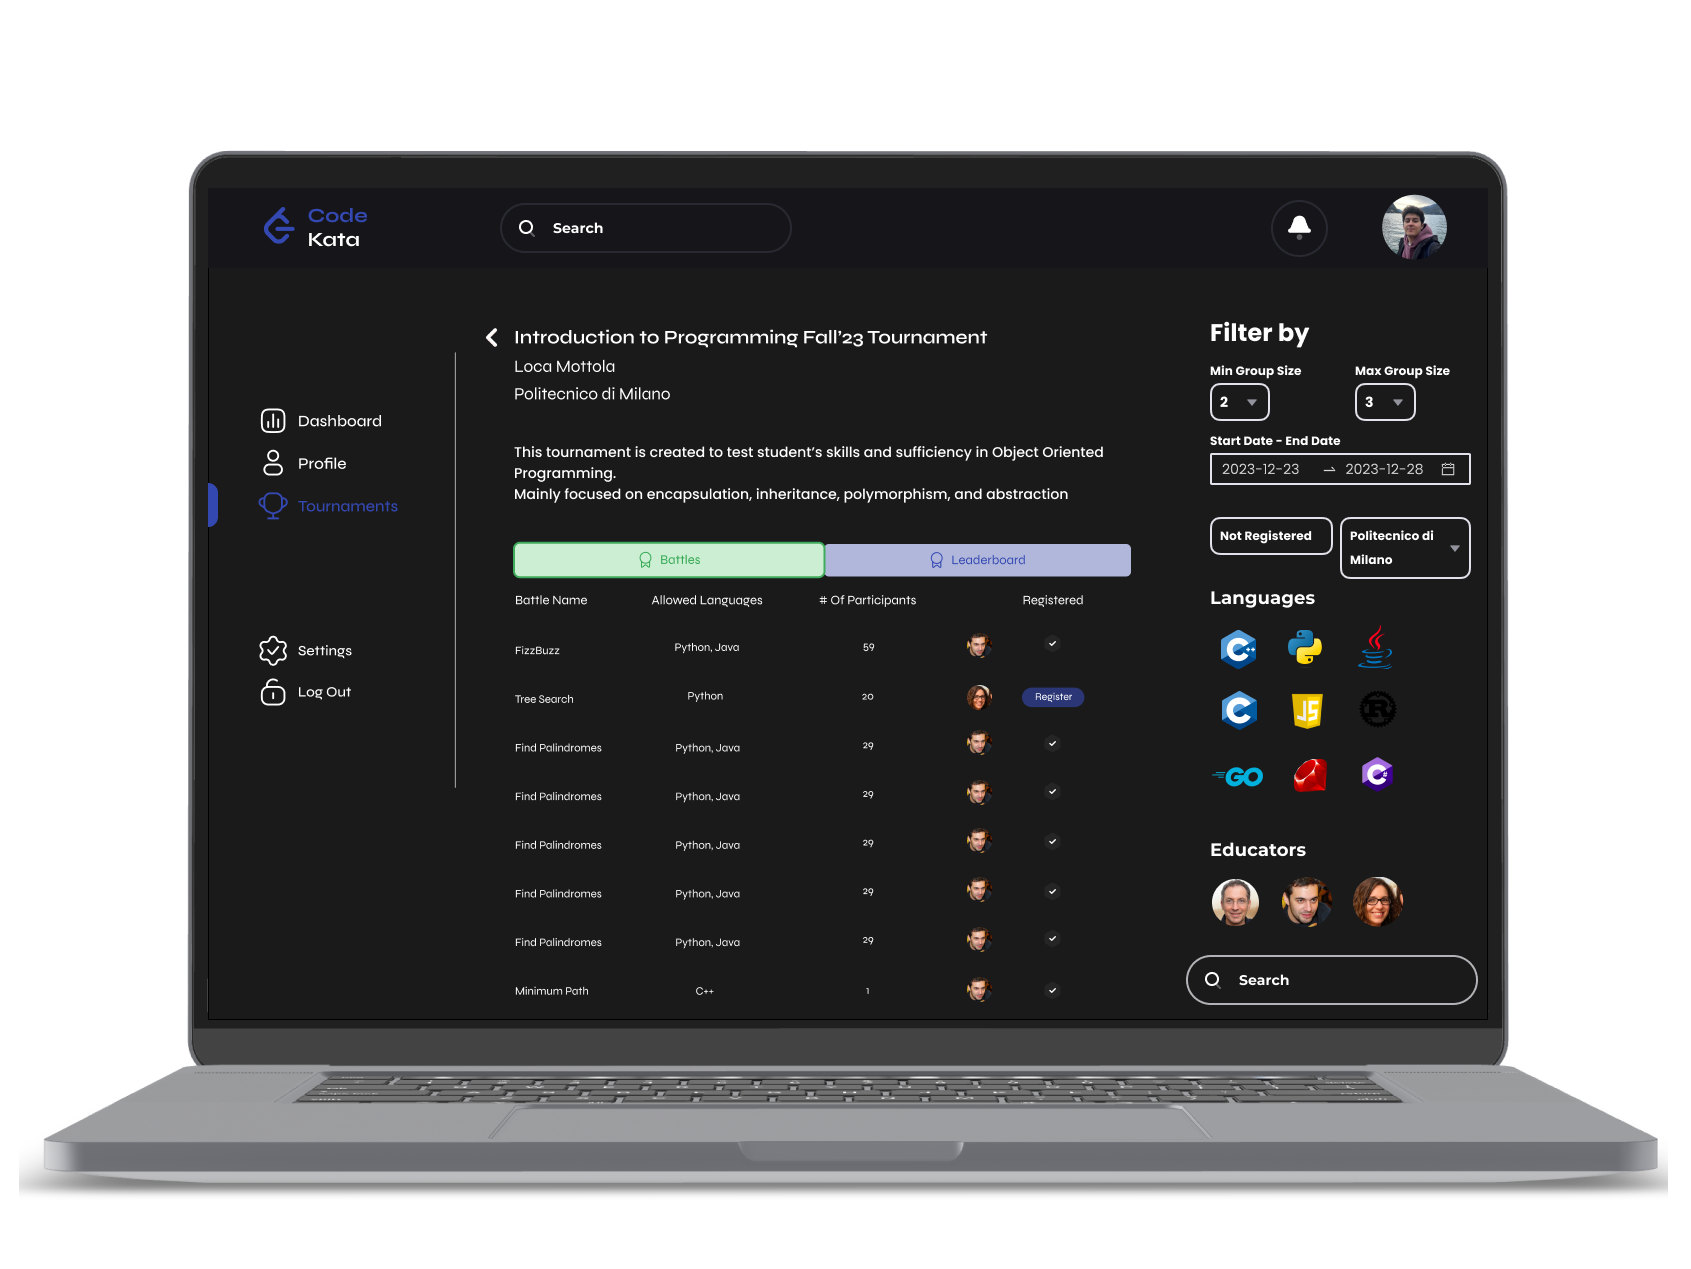
\includegraphics[scale=0.13]{Images/ui-ux/student_tournament/student_tournament_1.png}
%     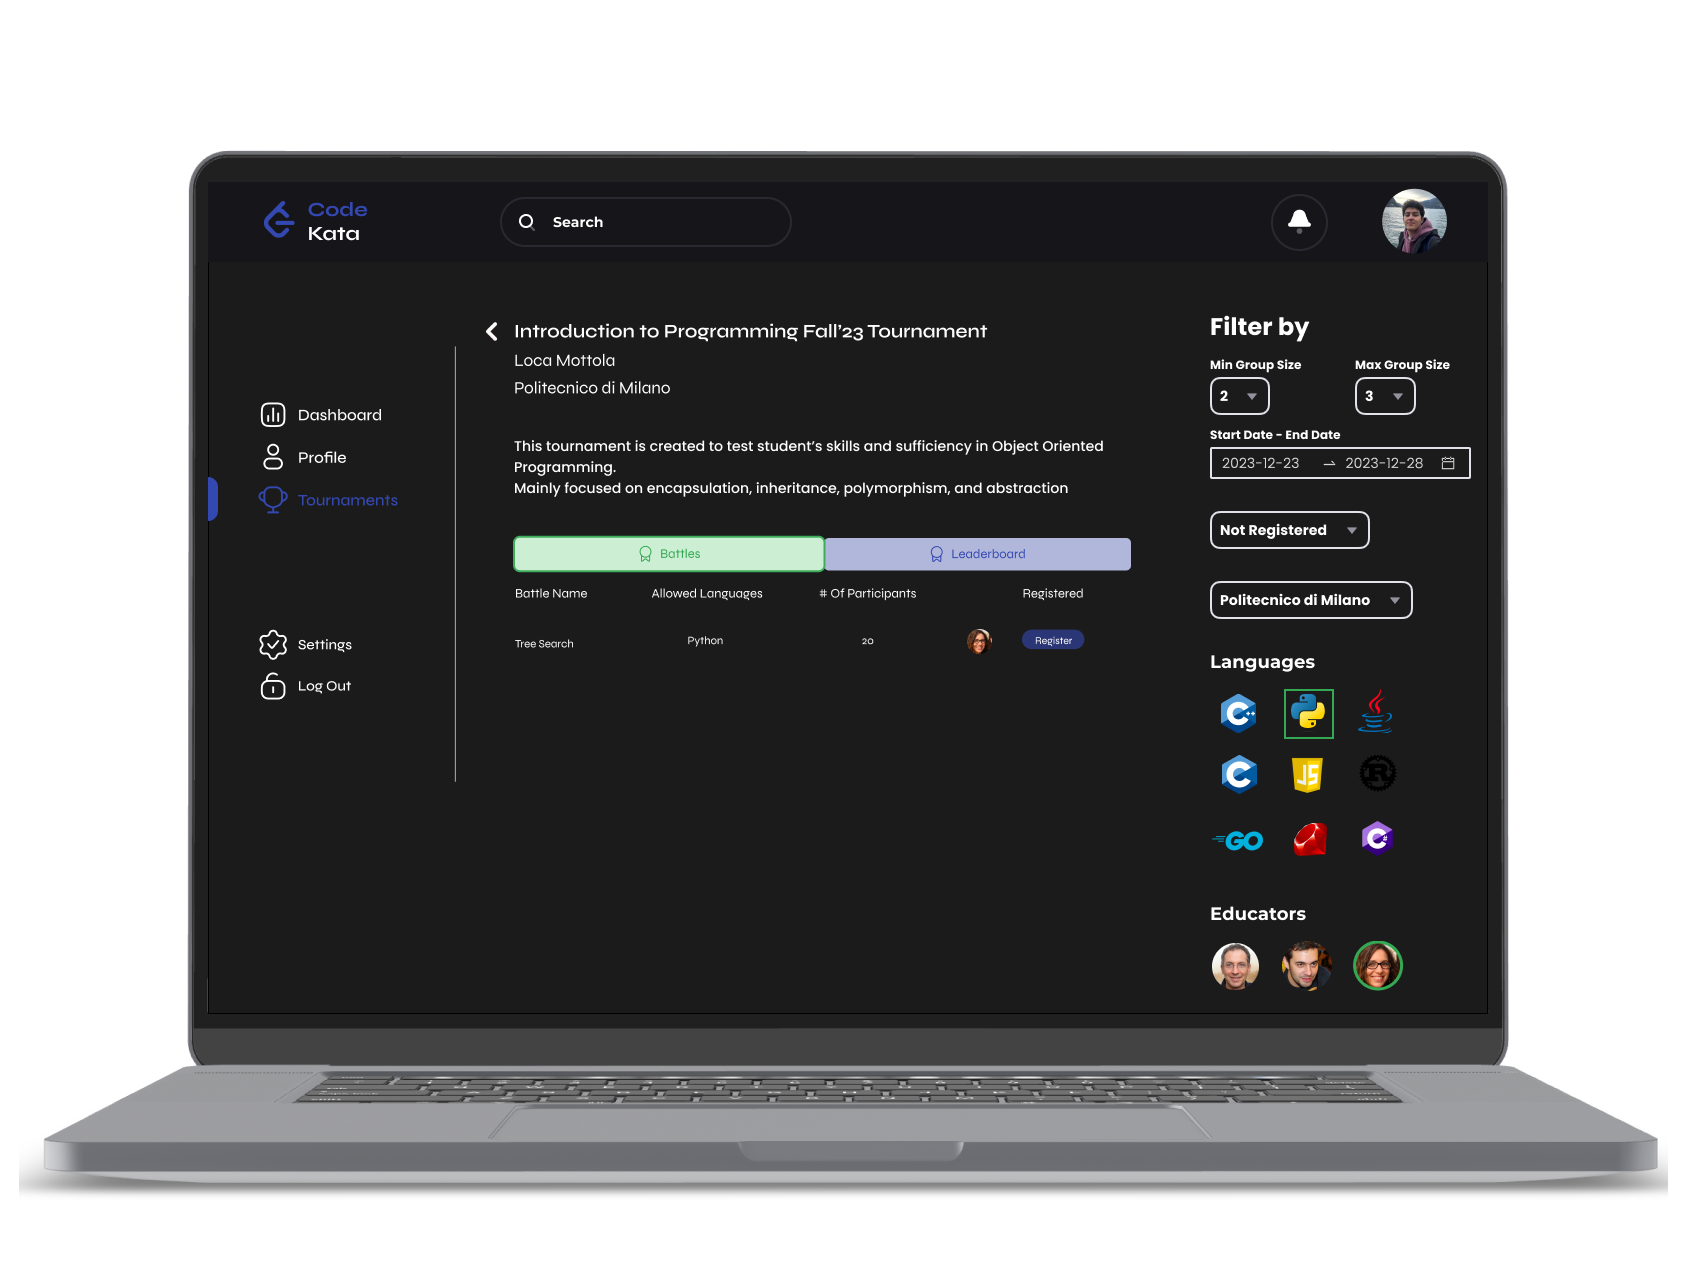
\includegraphics[scale=0.13]{Images/ui-ux/student_tournament/student_tournament_2.png}    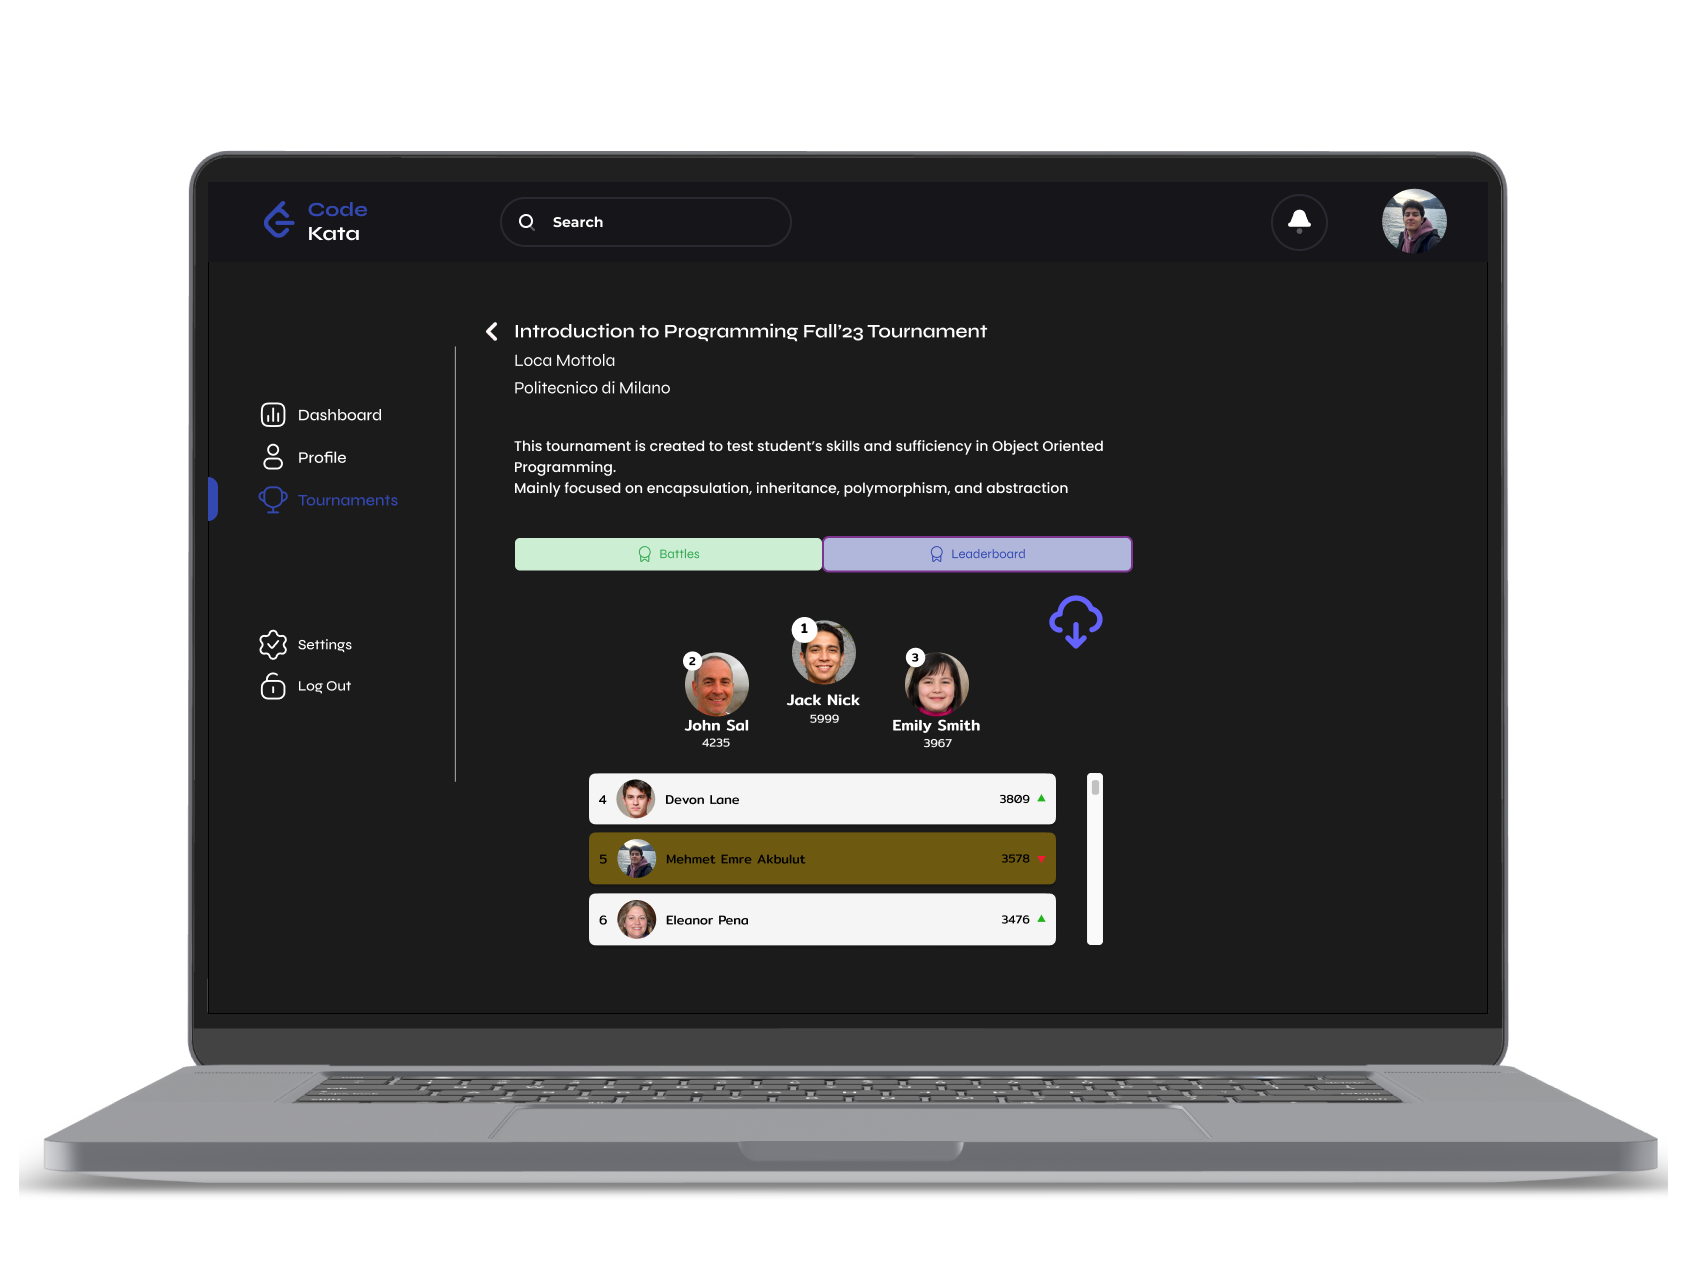
\includegraphics[scale=0.13]{Images/ui-ux/student_tournament/student_tournament_3.png} 
%     \\ (a) Student and A Tournament
% \end{center}
% \newpage
% \begin{center}
% 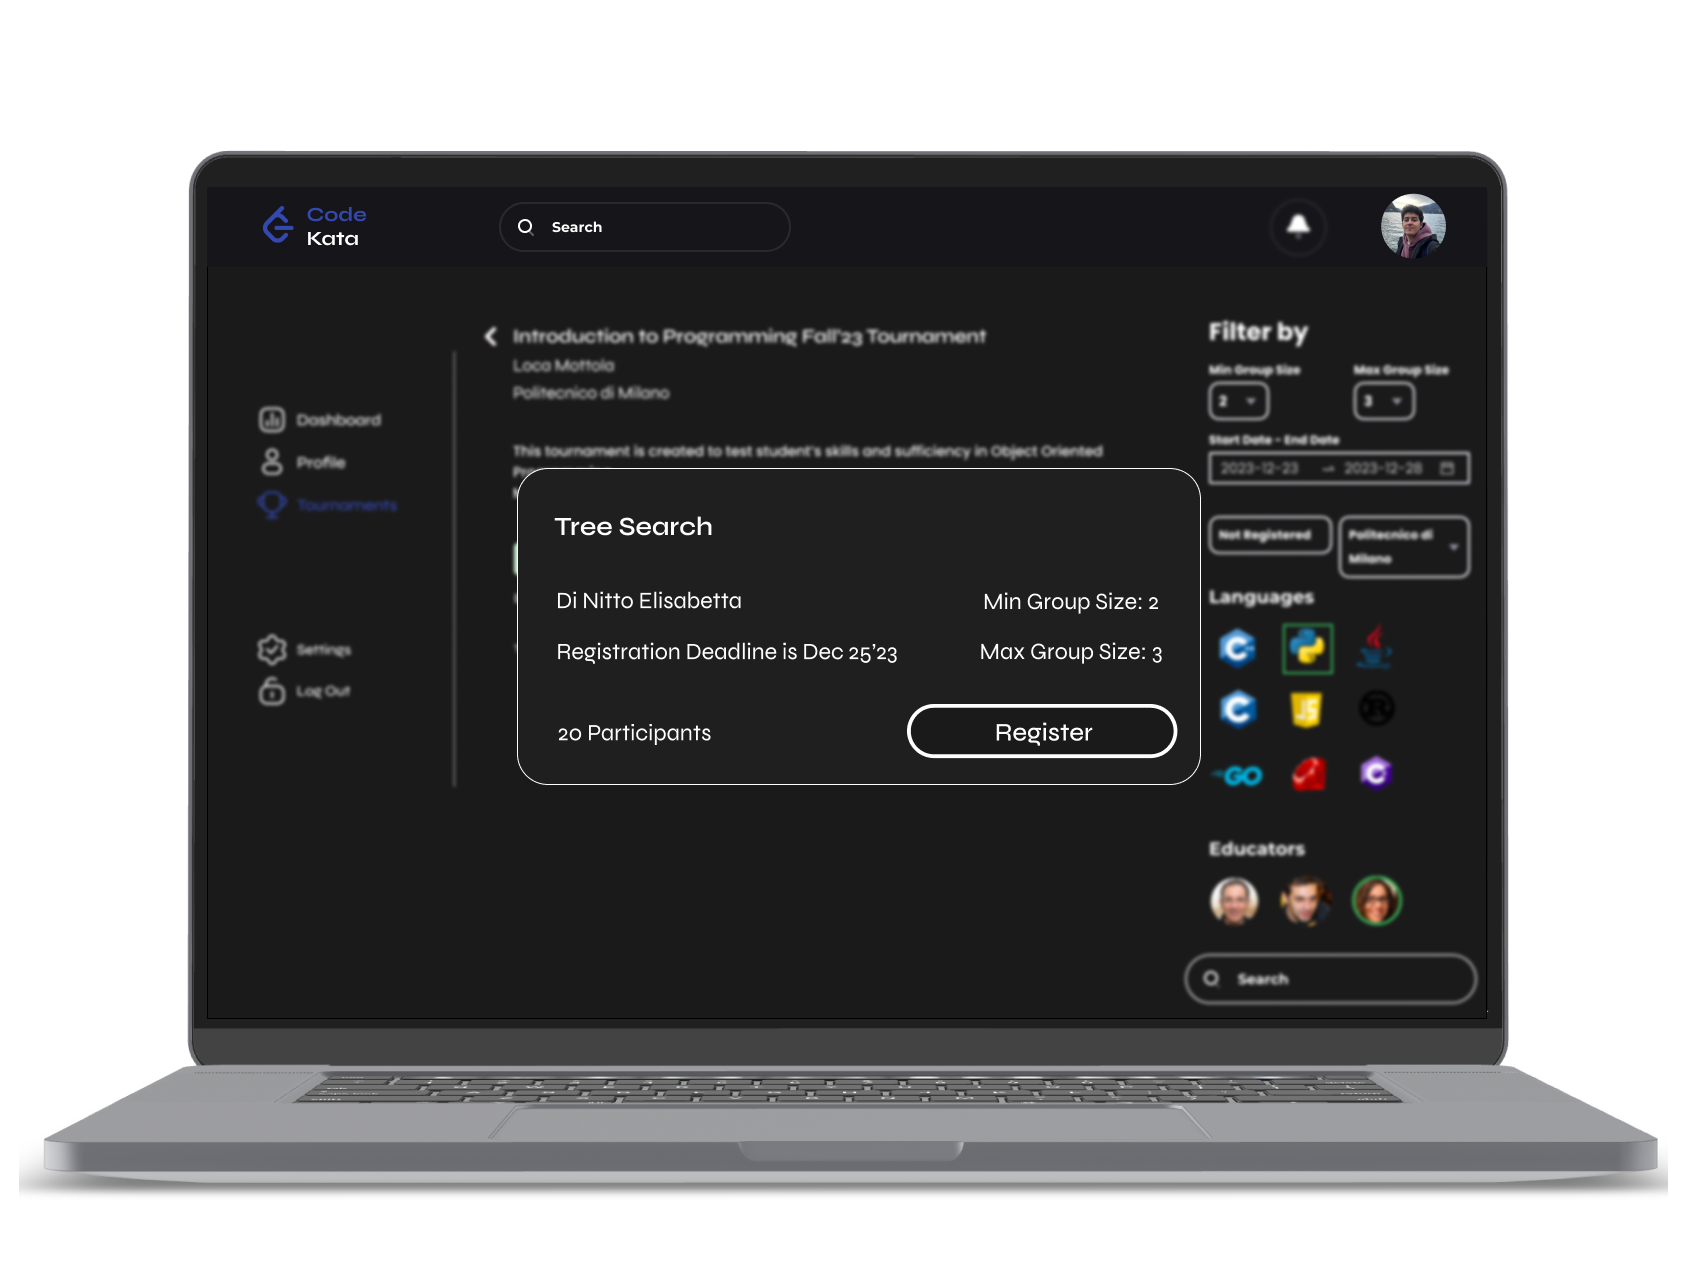
\includegraphics[scale=0.13]{Images/ui-ux/student_battle_register/student_battle_register_1.png}
% 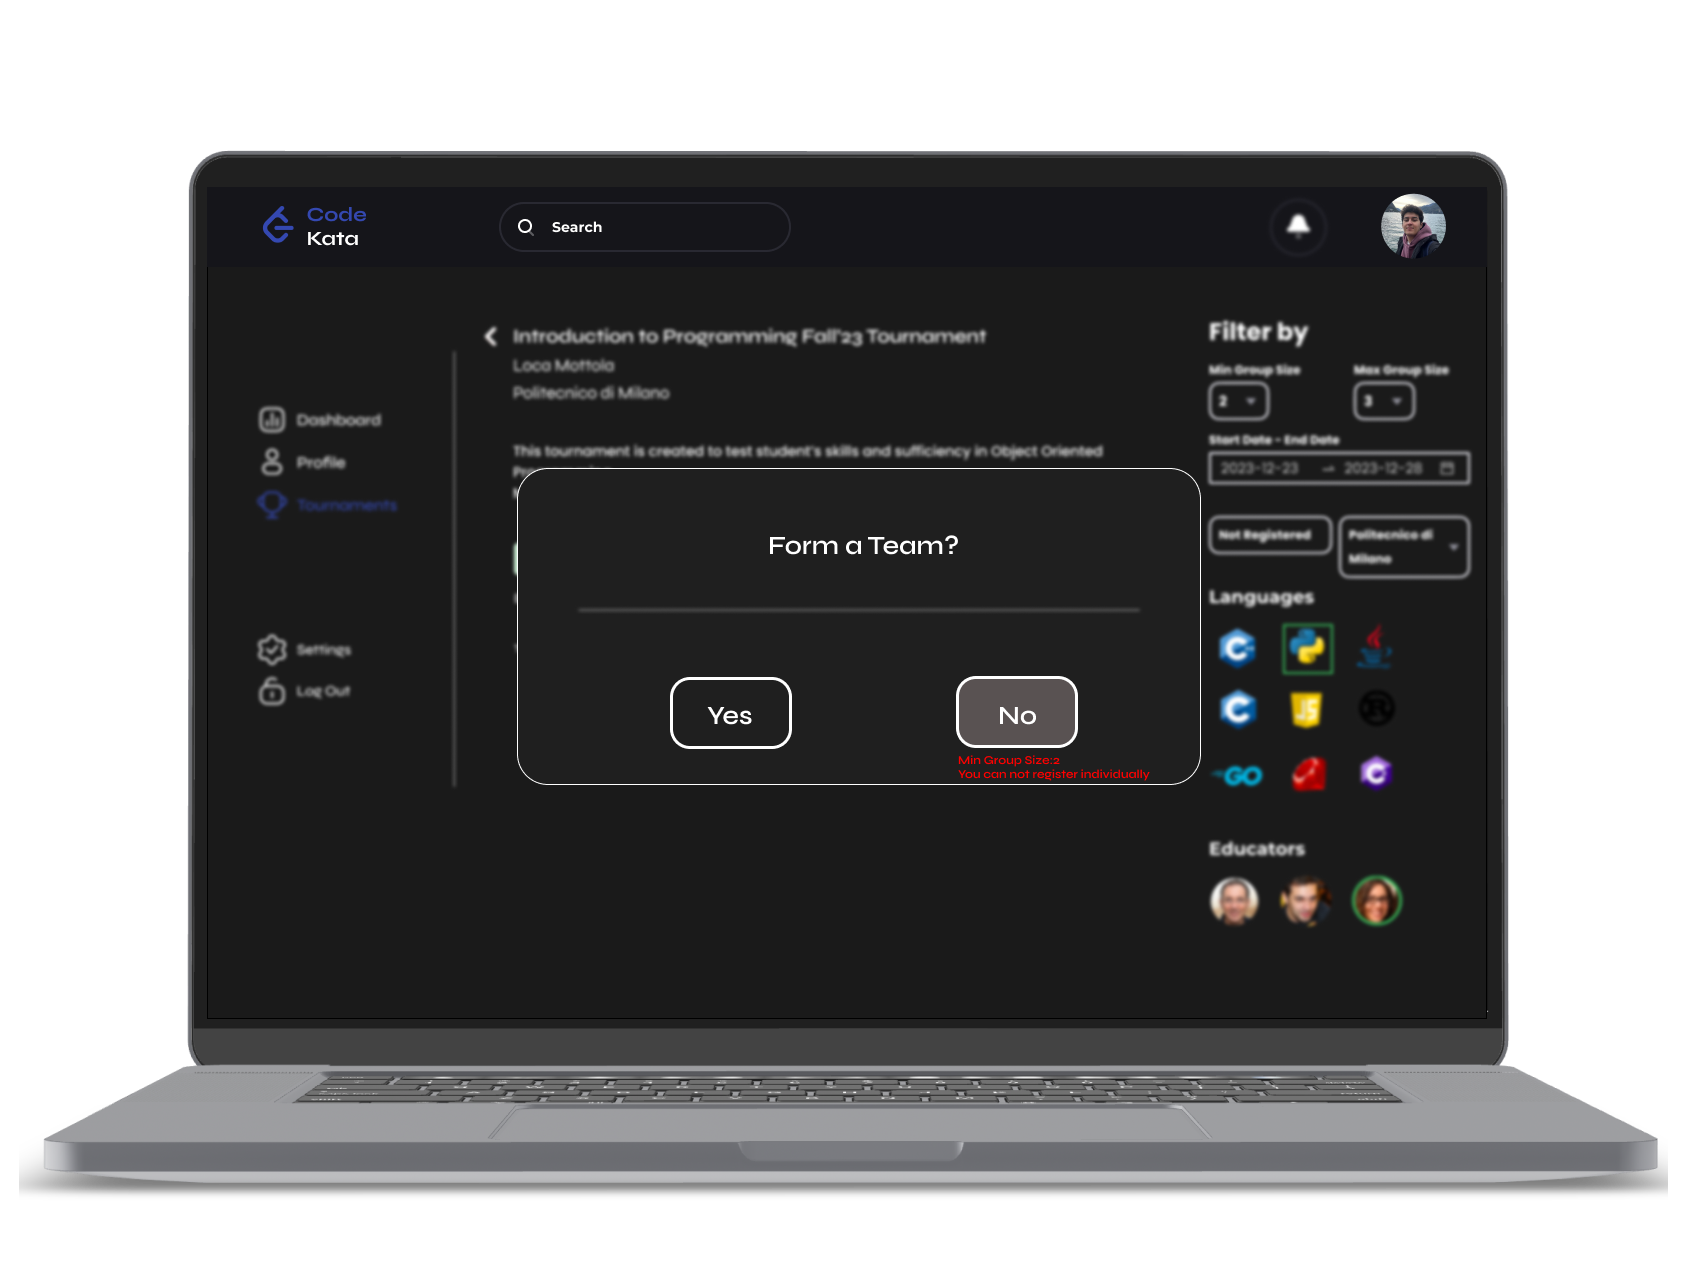
\includegraphics[scale=0.13]{Images/ui-ux/student_battle_register/student_battle_register_2.png}
% 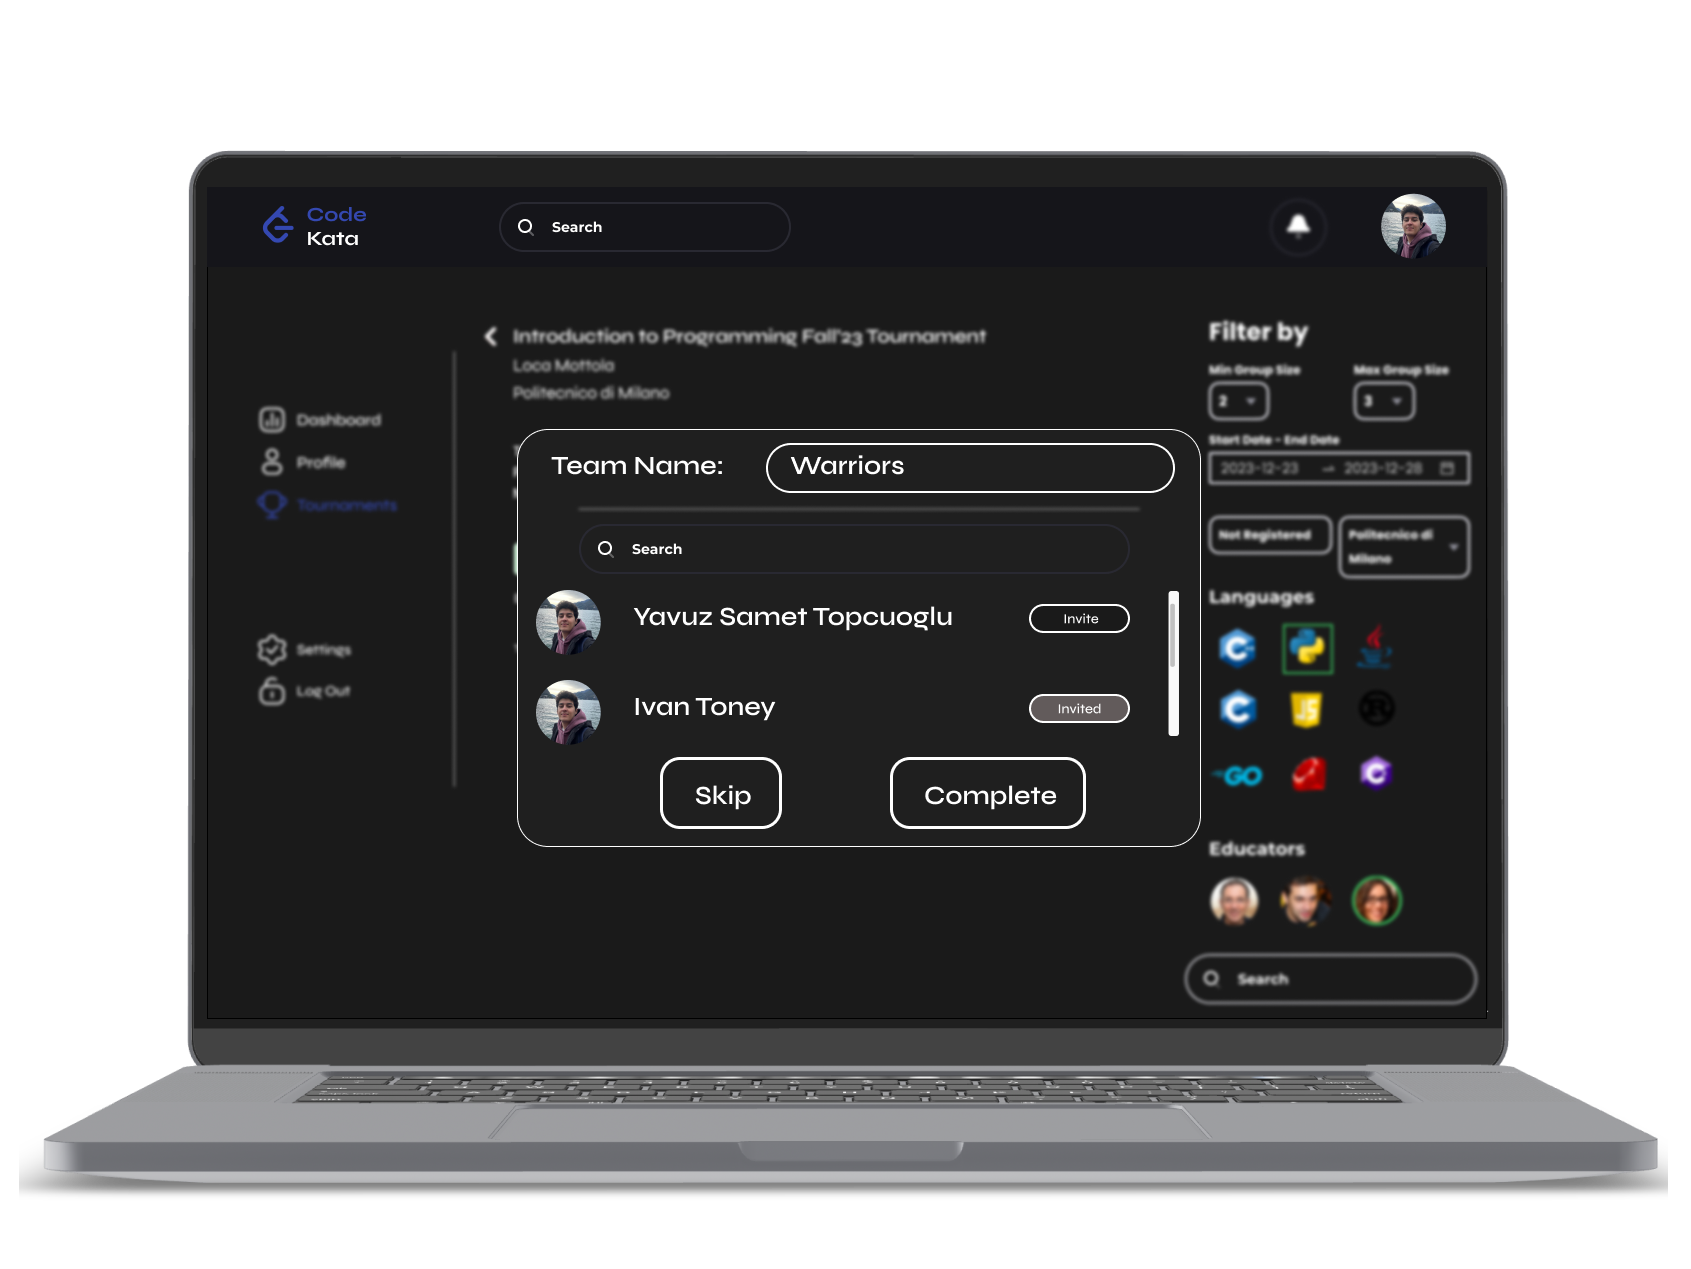
\includegraphics[scale=0.13]{Images/ui-ux/student_battle_register/student_battle_register_3.png}
% \\ (a) Student Registers Battle
% \end{center}
% \newpage
% \begin{center}
% 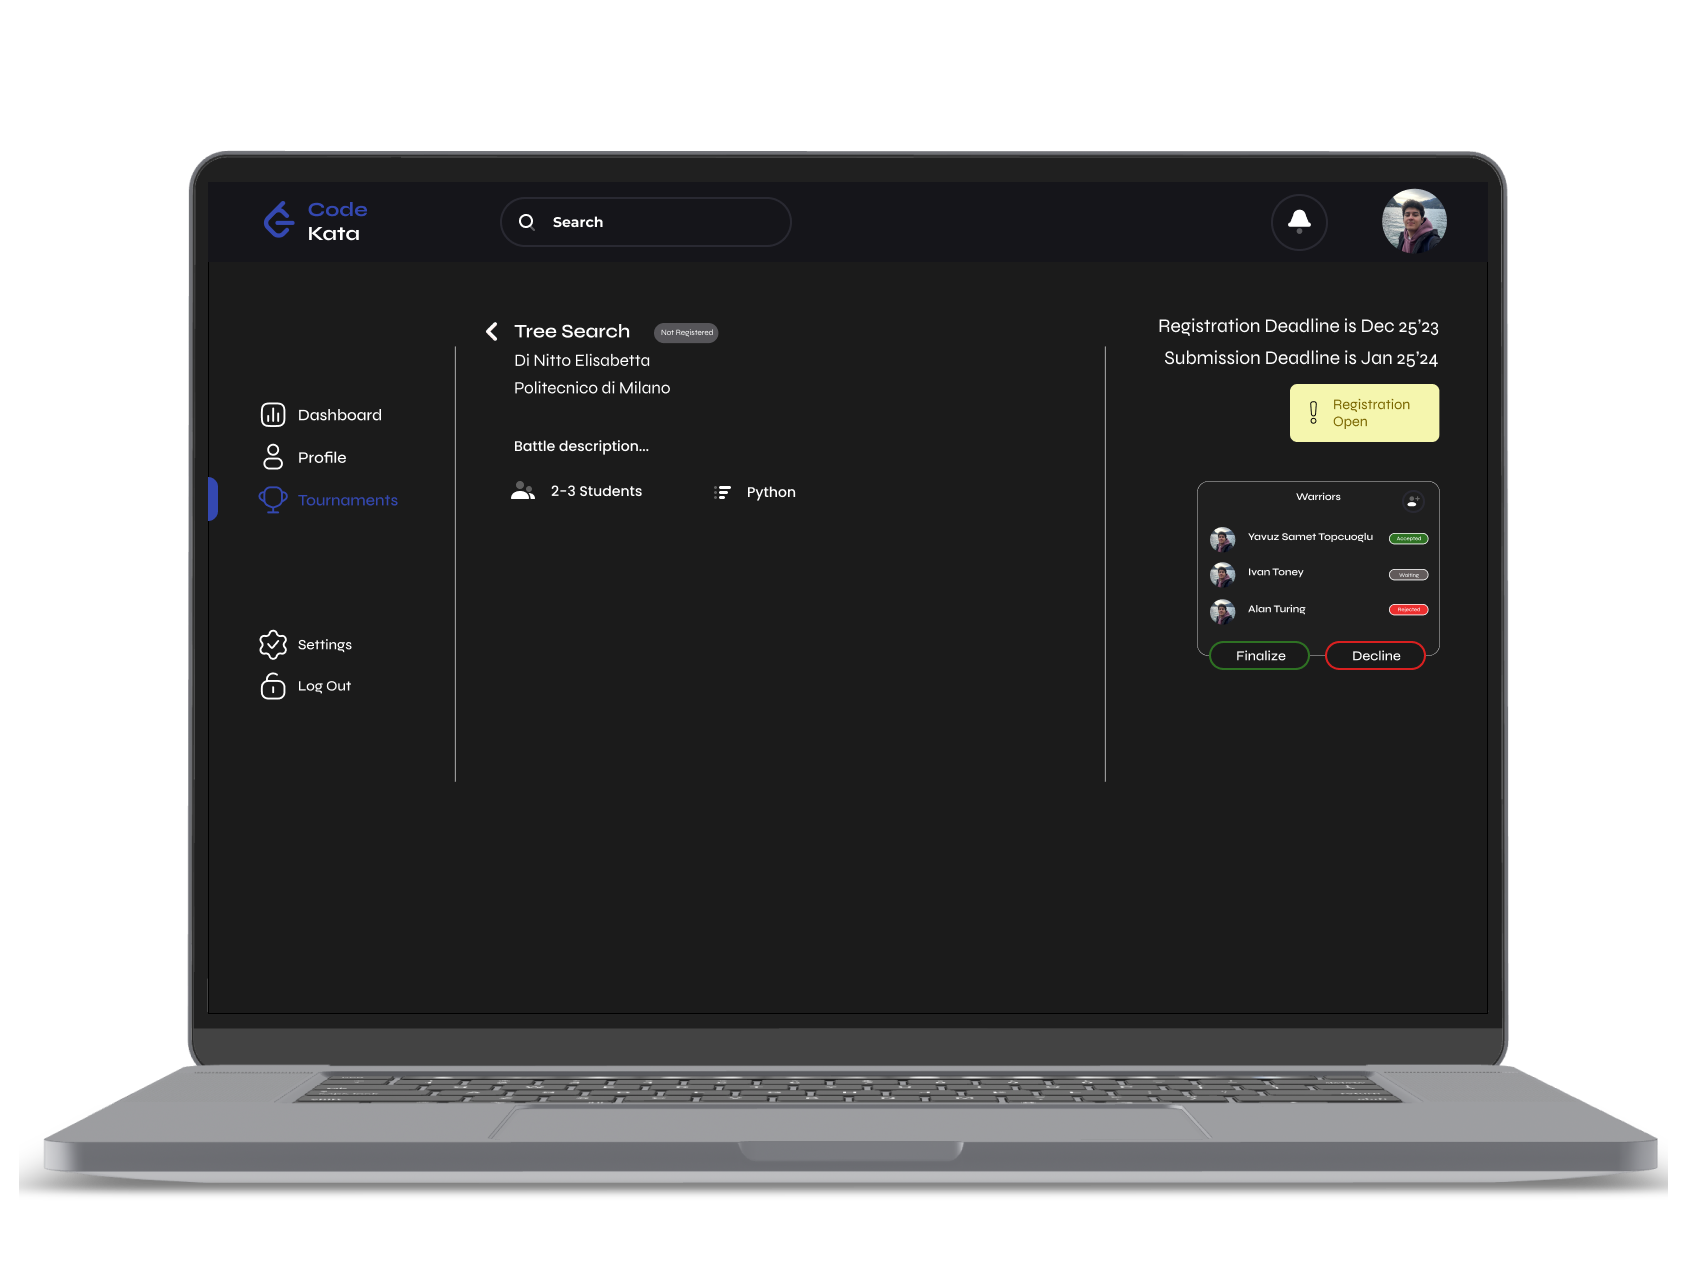
\includegraphics[scale=0.13]{Images/ui-ux/student_battle/student_battle_1.png}
% 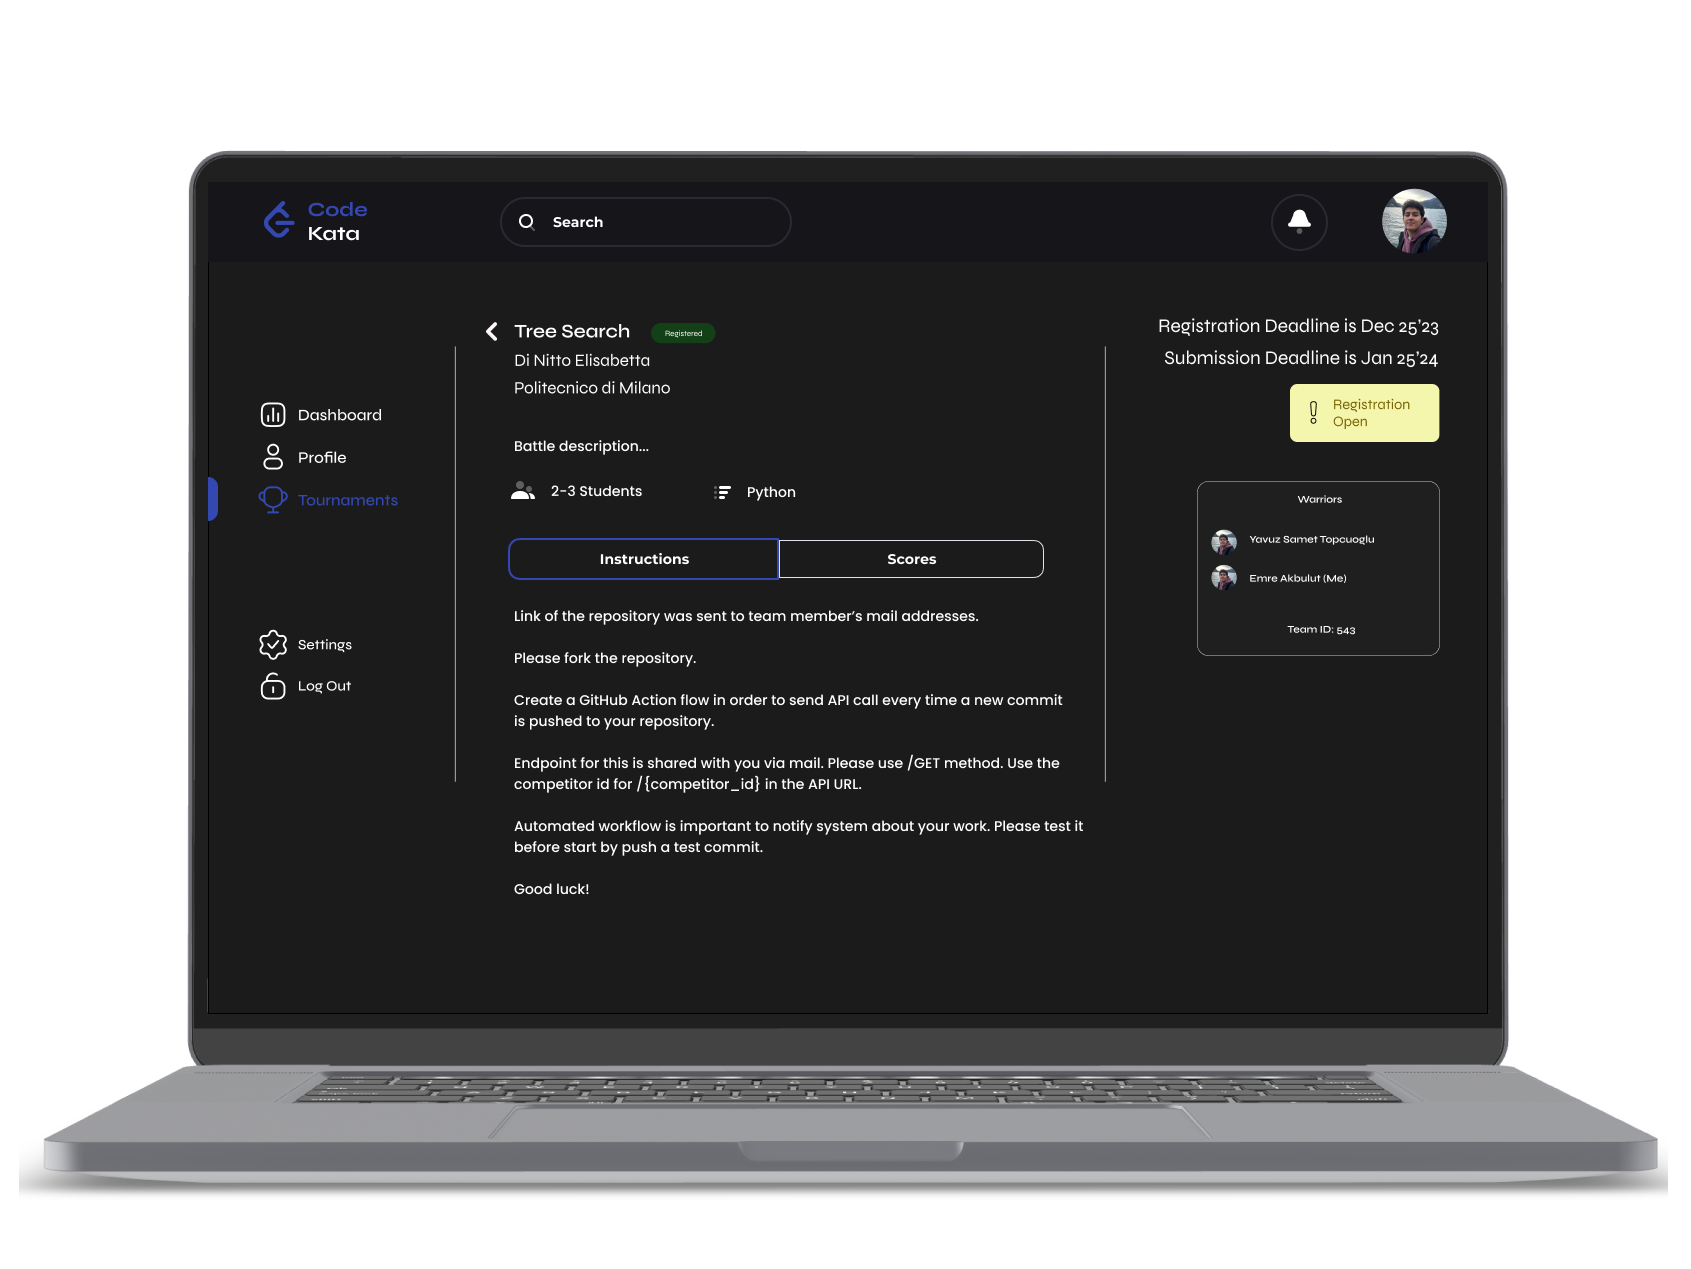
\includegraphics[scale=0.13]{Images/ui-ux/student_battle/student_battle_2.png}
% 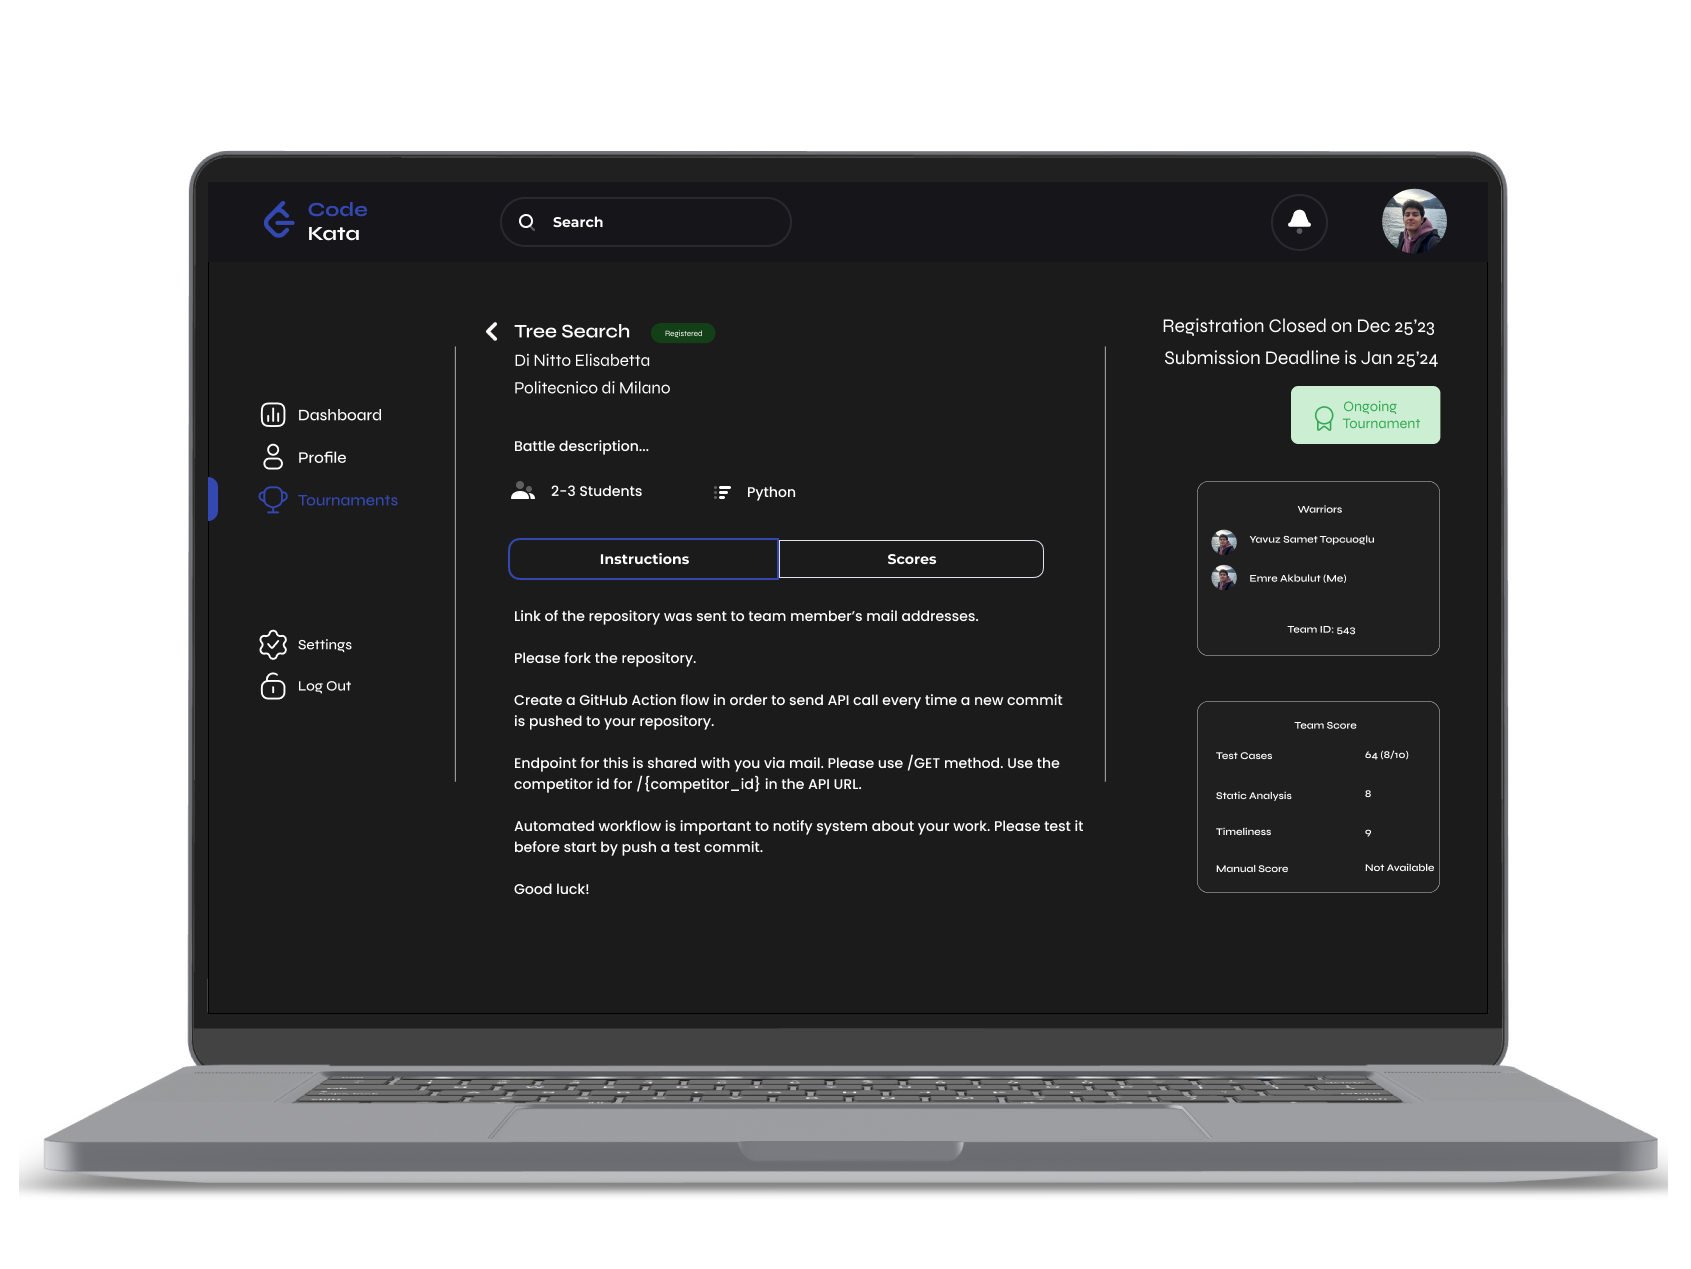
\includegraphics[scale=0.13]{Images/ui-ux/student_battle/student_battle_3.png}
% 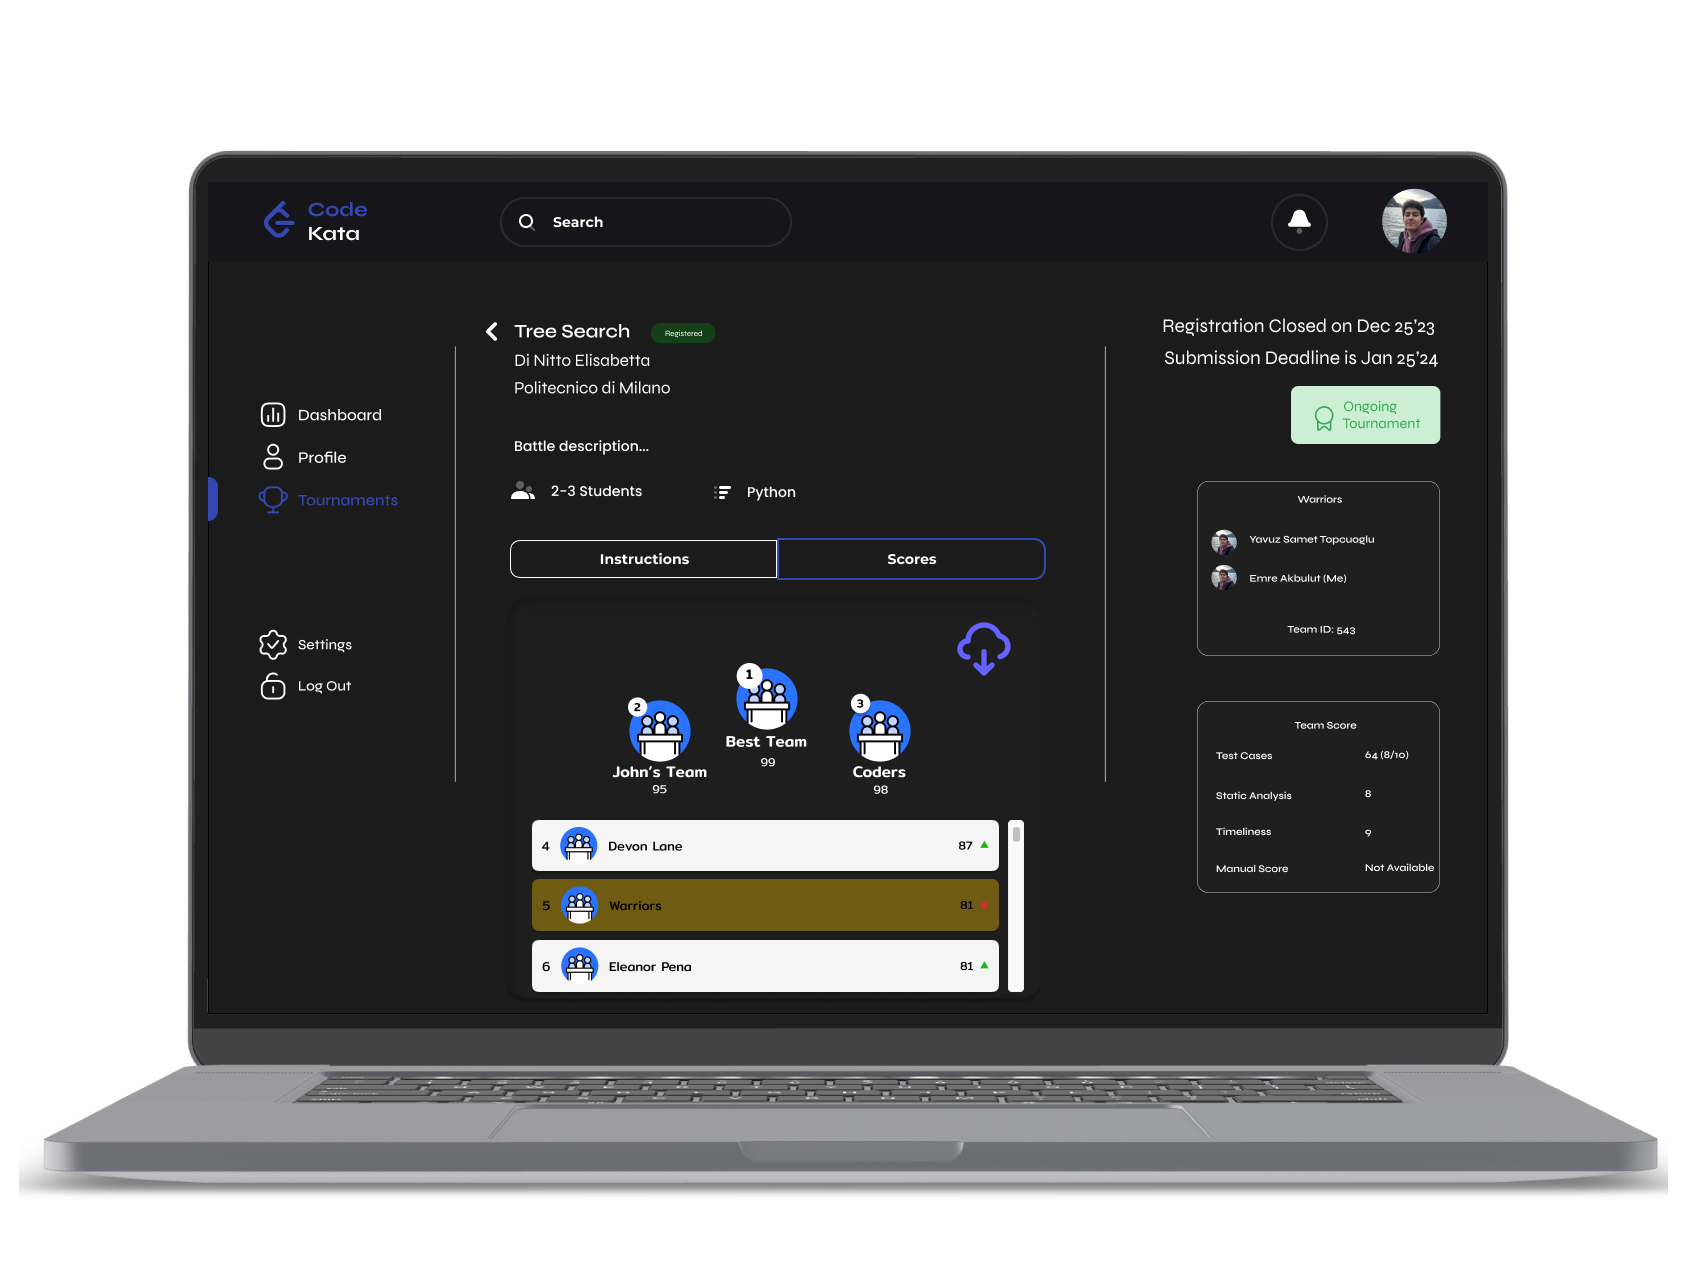
\includegraphics[scale=0.13]{Images/ui-ux/student_battle/student_battle_4.png}
%       (a) Battle Screen for Student
% \end{center}

% \begin{center}
% 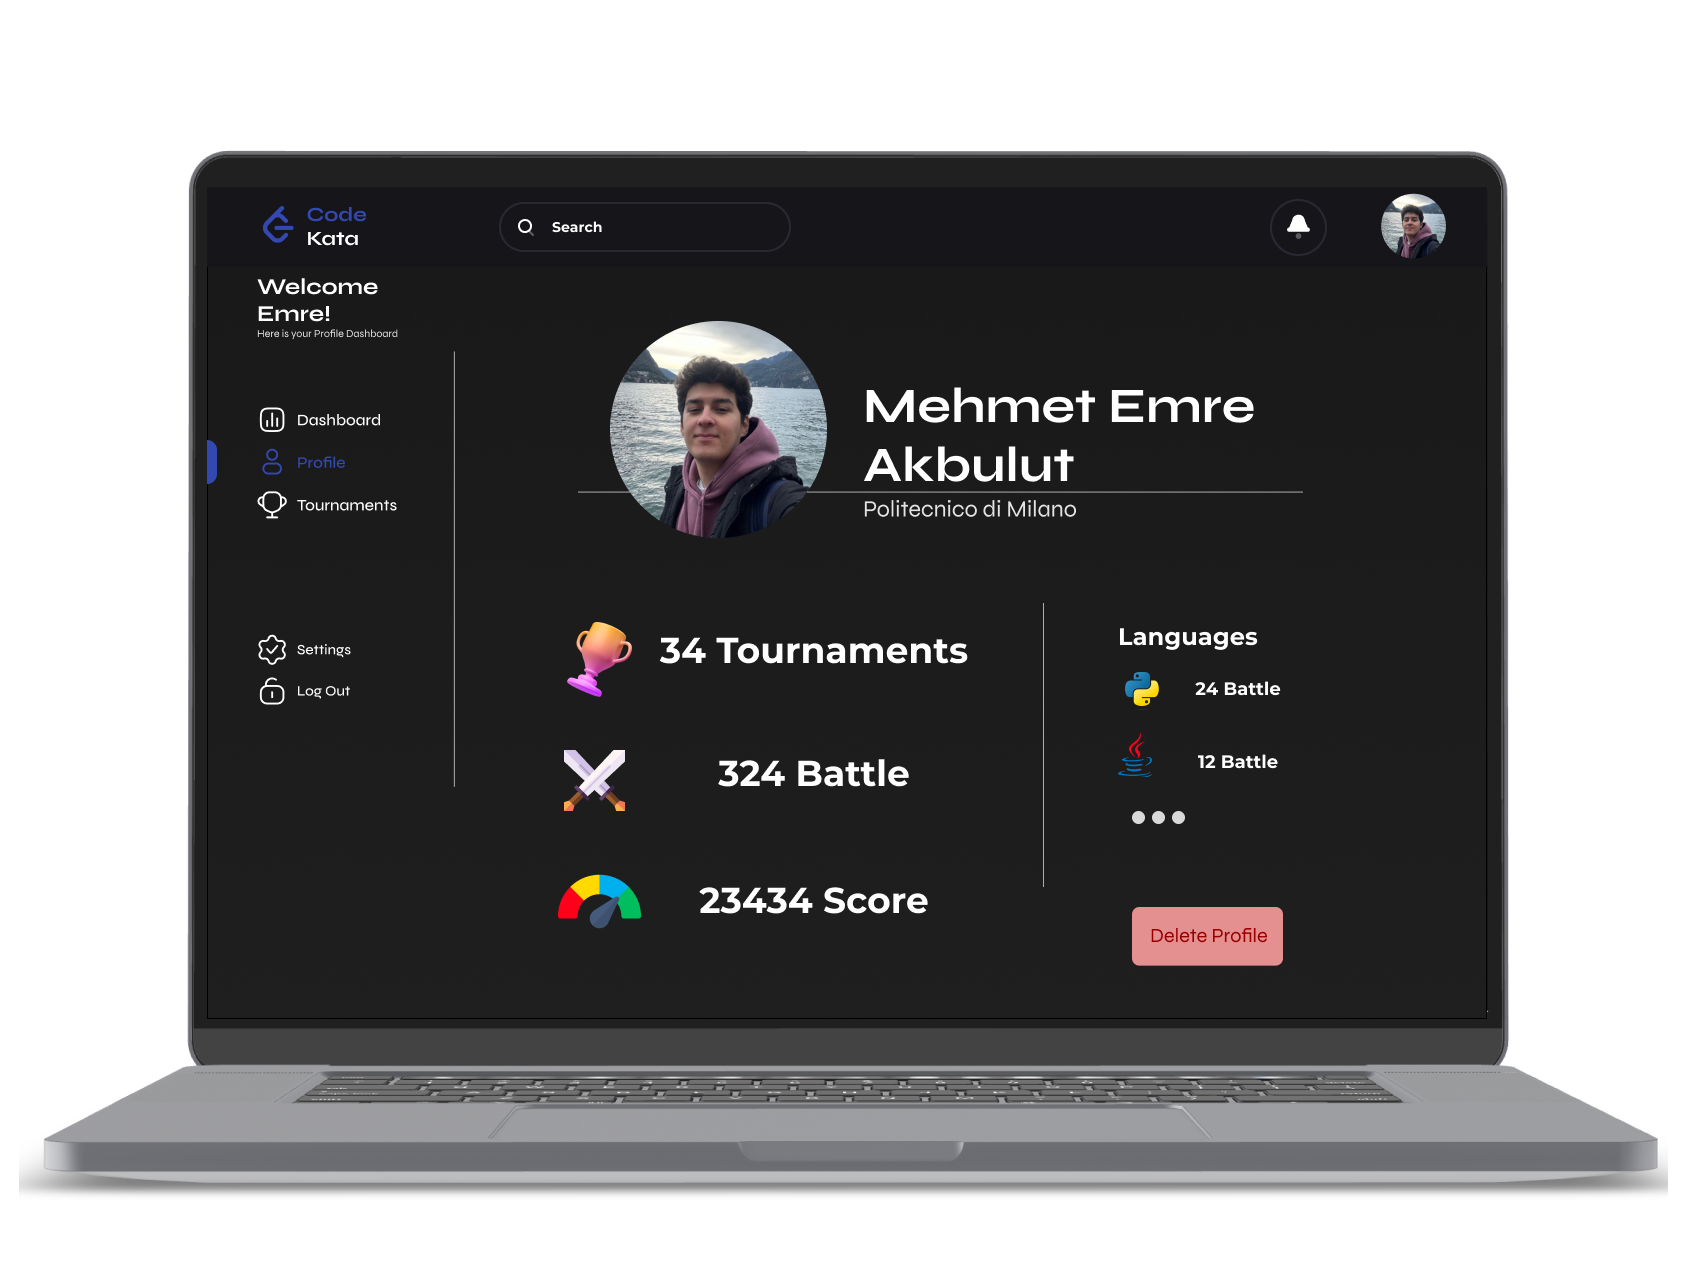
\includegraphics[scale=0.13]{Images/ui-ux/student_profile_settings/student_profile.png}
% 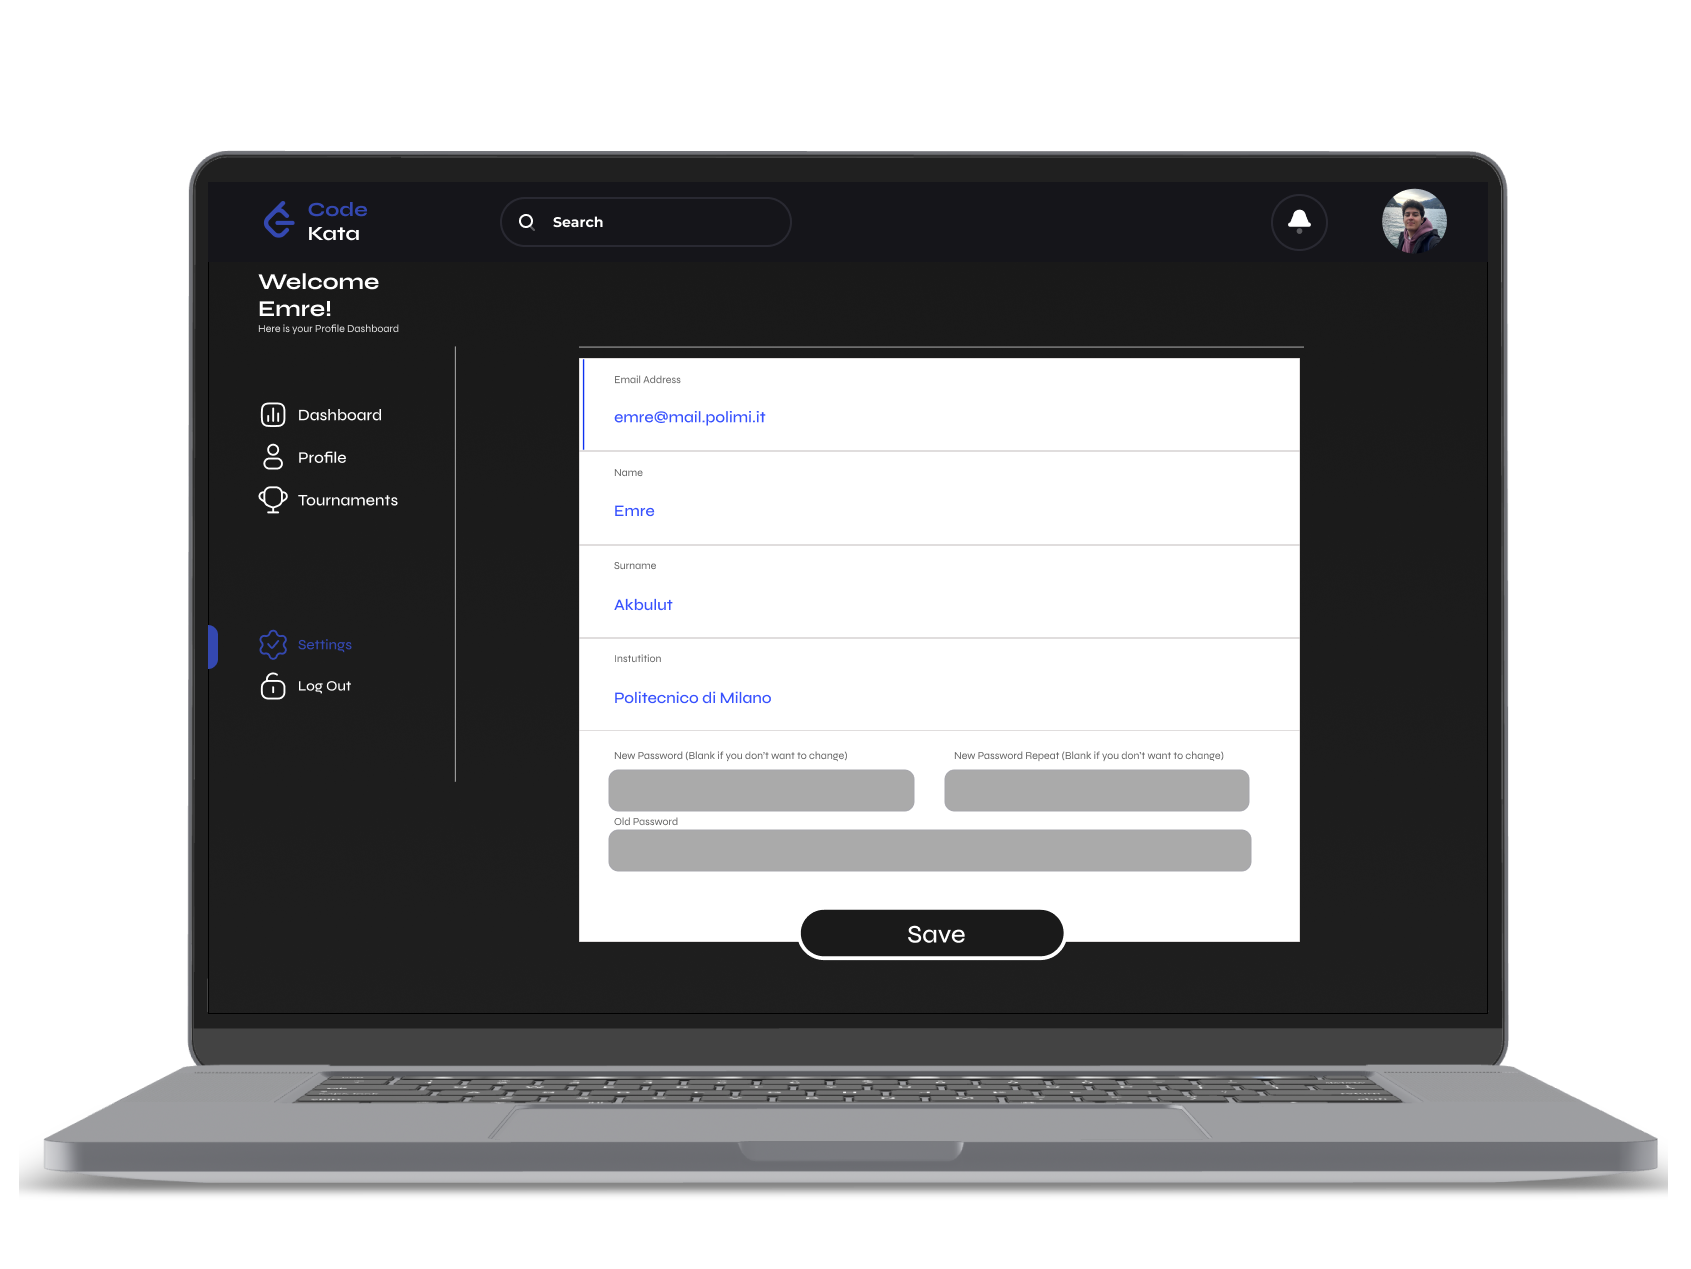
\includegraphics[scale=0.13]{Images/ui-ux/student_profile_settings/student_settings.png}
%         (a) Profile and Settings for Student
% \end{center}
% \newpage
% \begin{center}
% 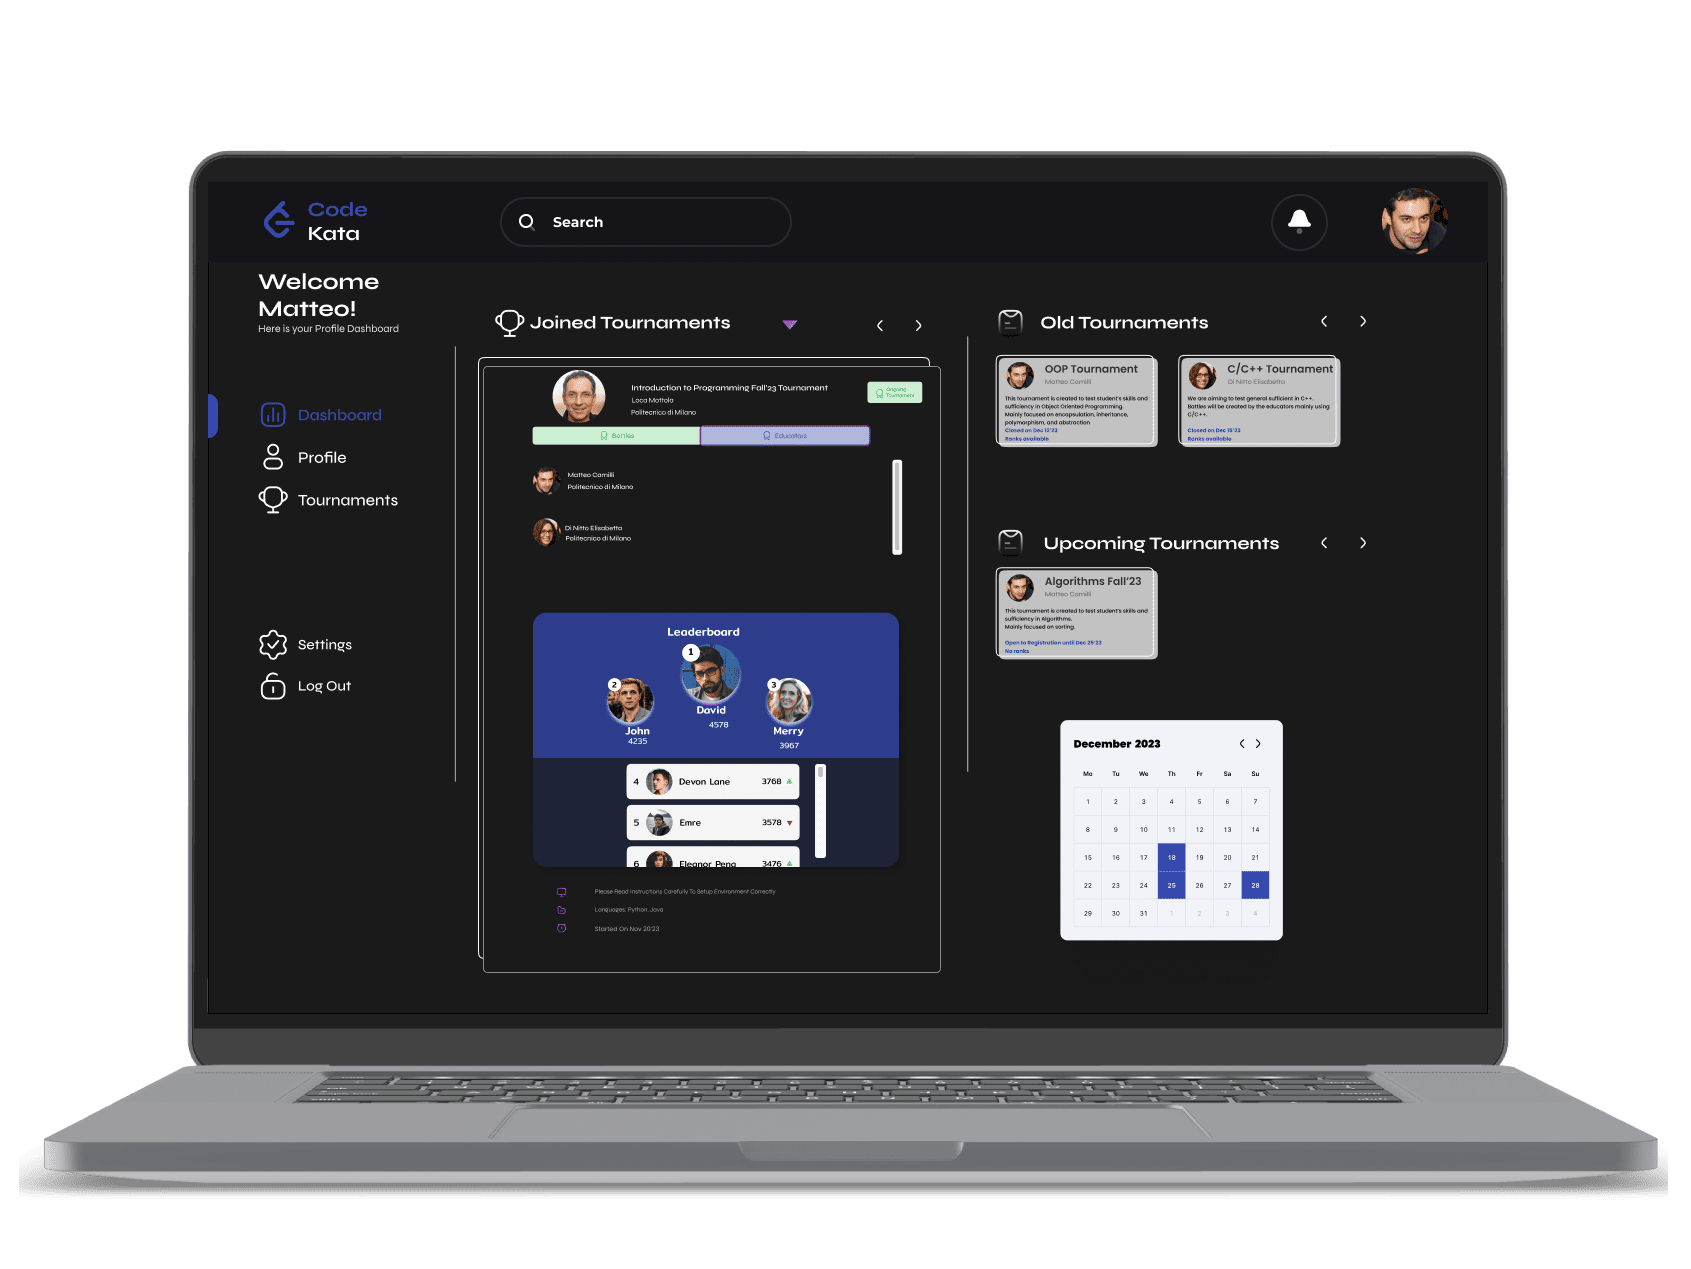
\includegraphics[scale=0.13]{Images/ui-ux/educator_dashboard/educator_dashboard_1.png}
% 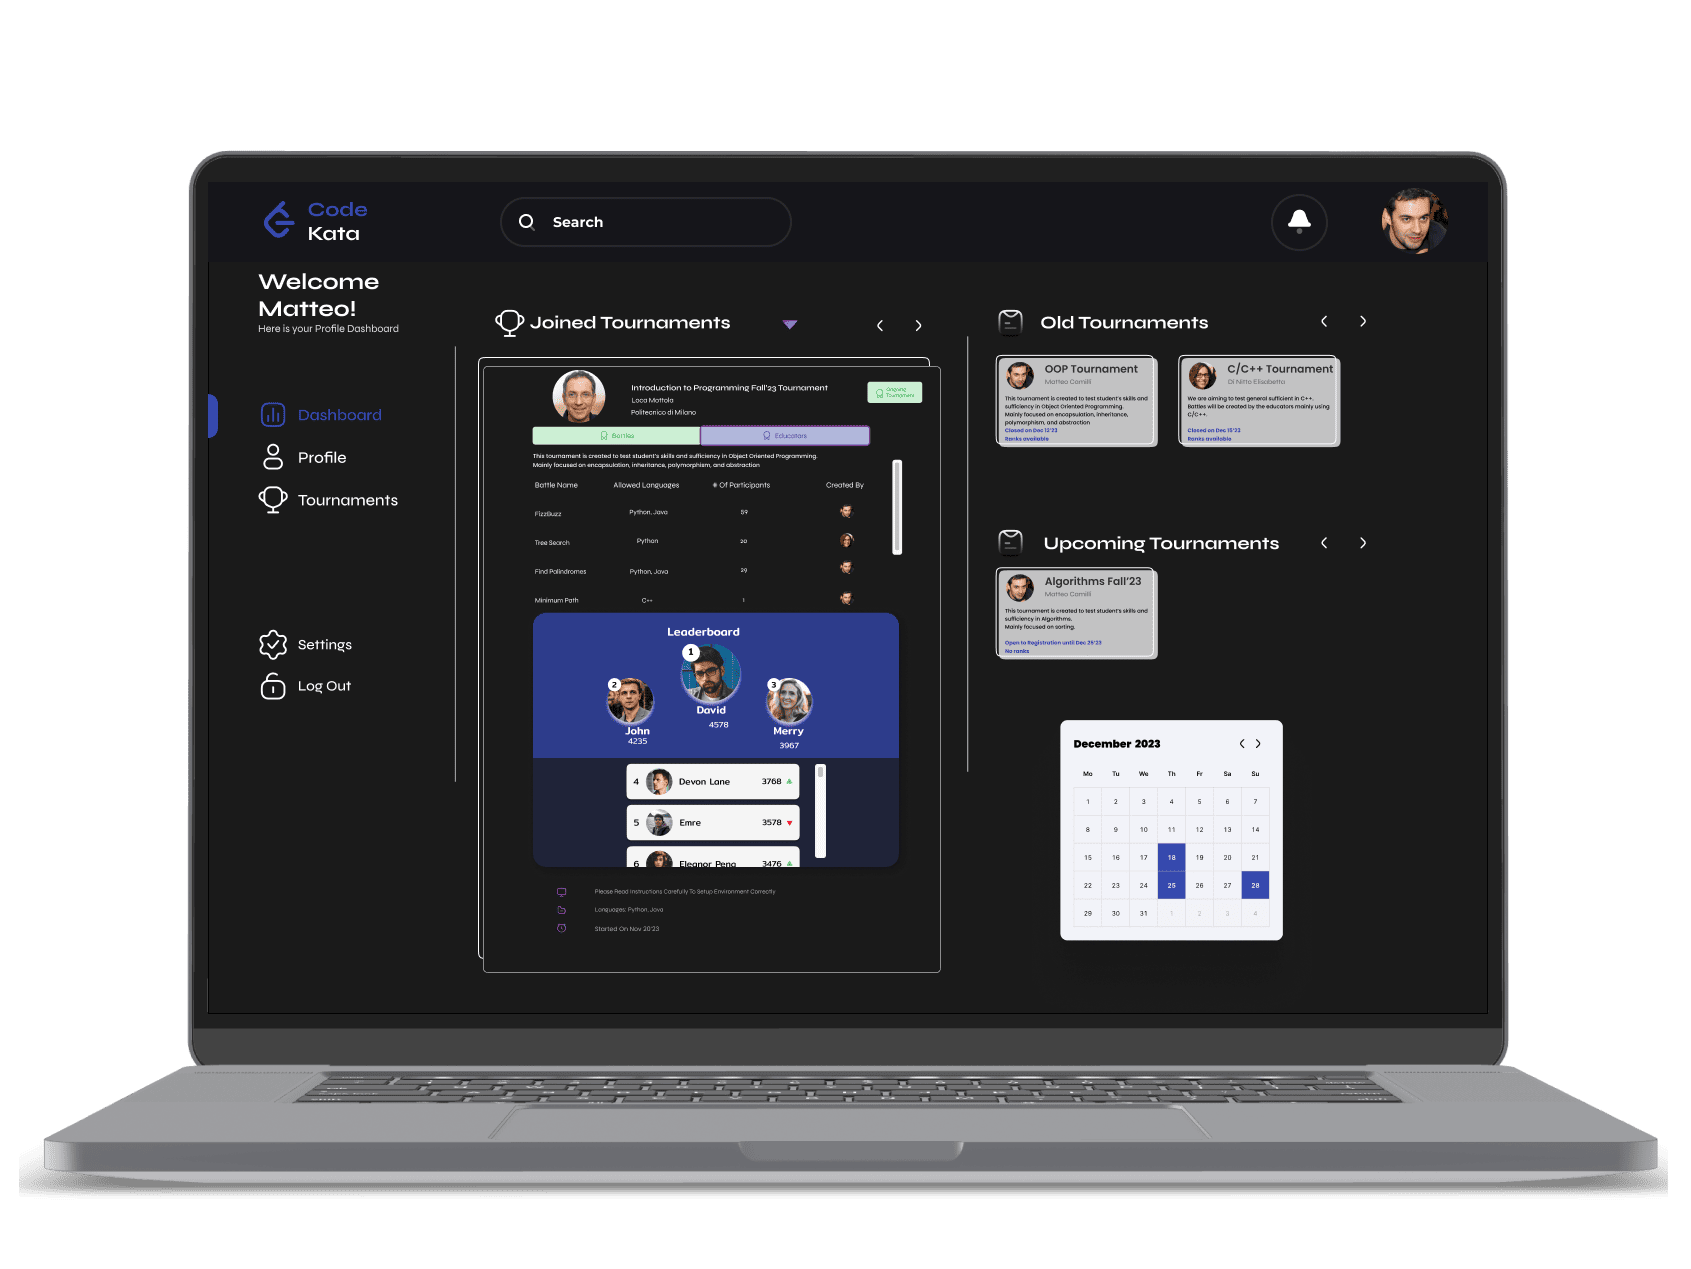
\includegraphics[scale=0.13]{Images/ui-ux/educator_dashboard/educator_dashboard_2.png}
% 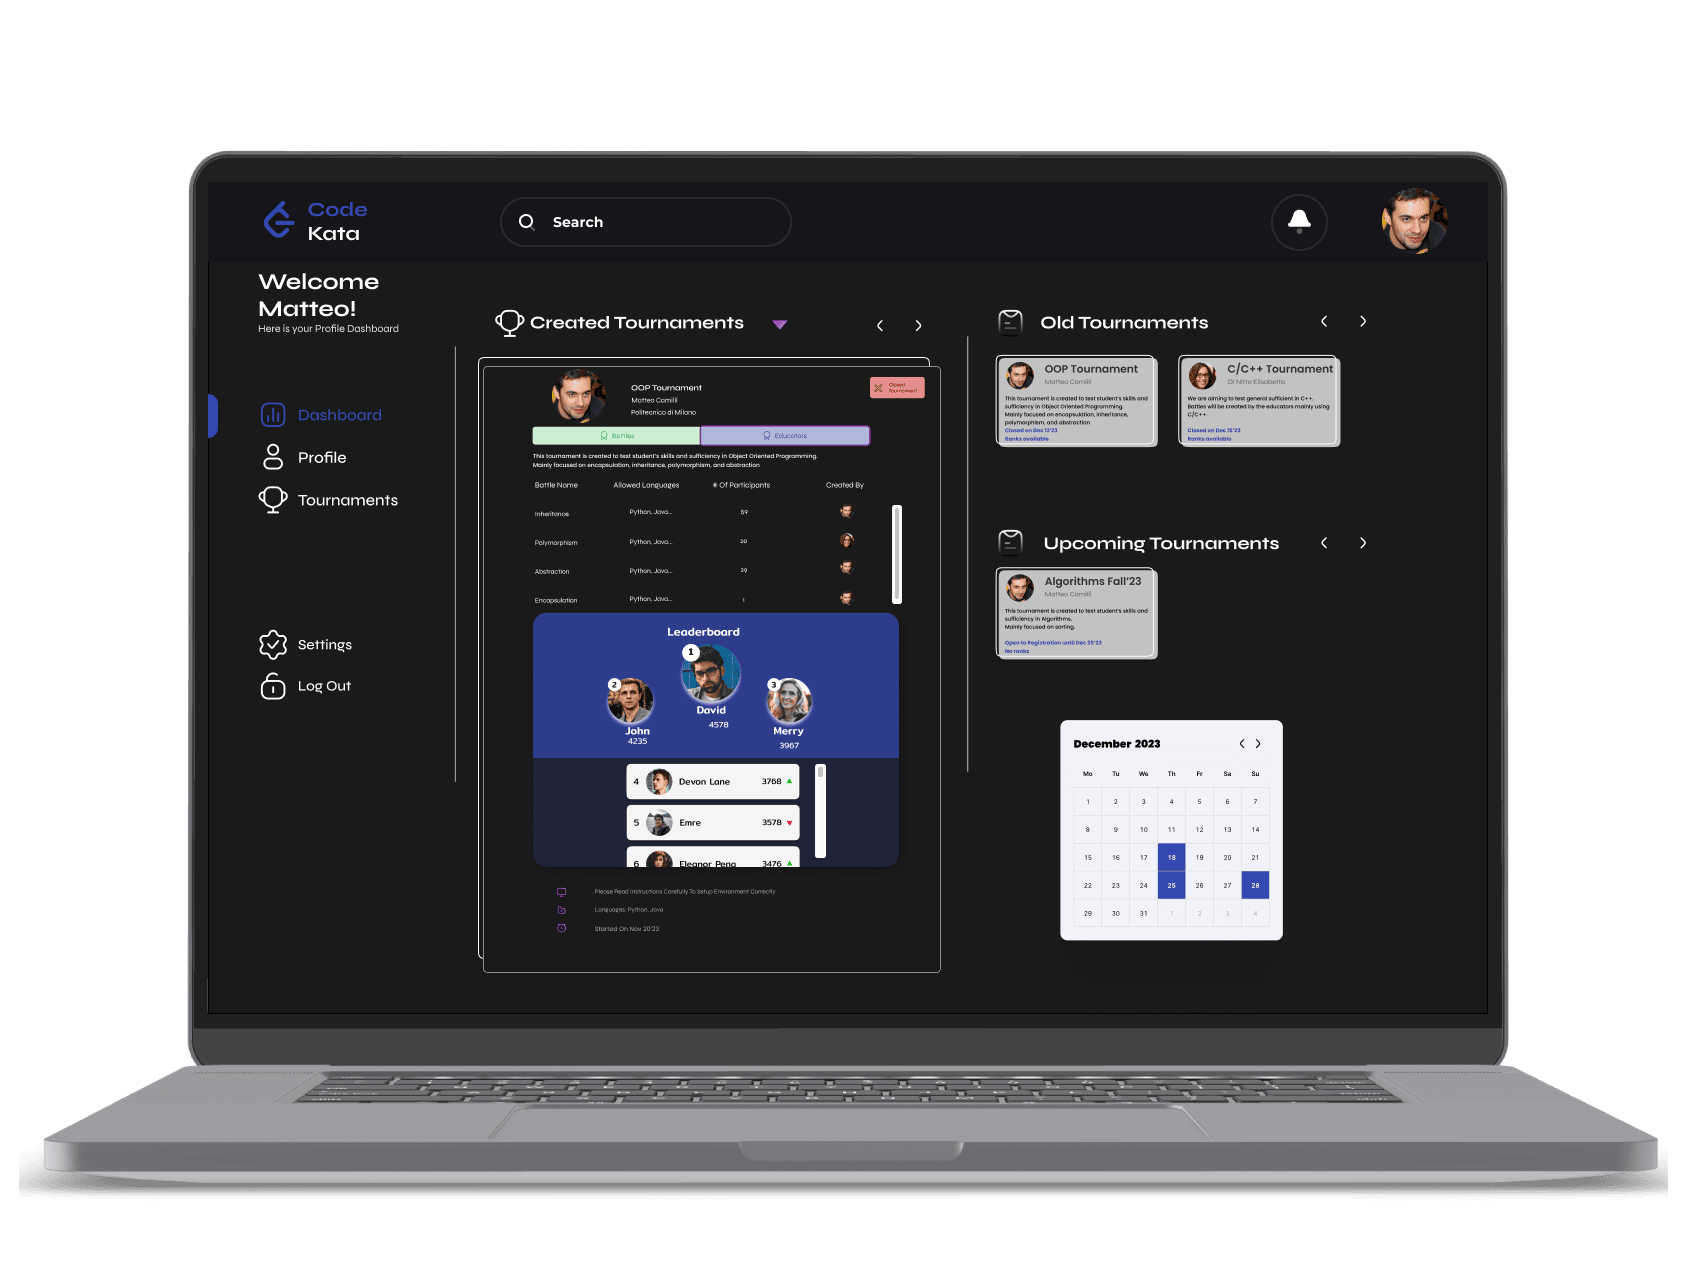
\includegraphics[scale=0.13]{Images/ui-ux/educator_dashboard/educator_dashboard_3.png}
% \\ (a) Educator Dashboard
% \end{center}
% \begin{center}
% 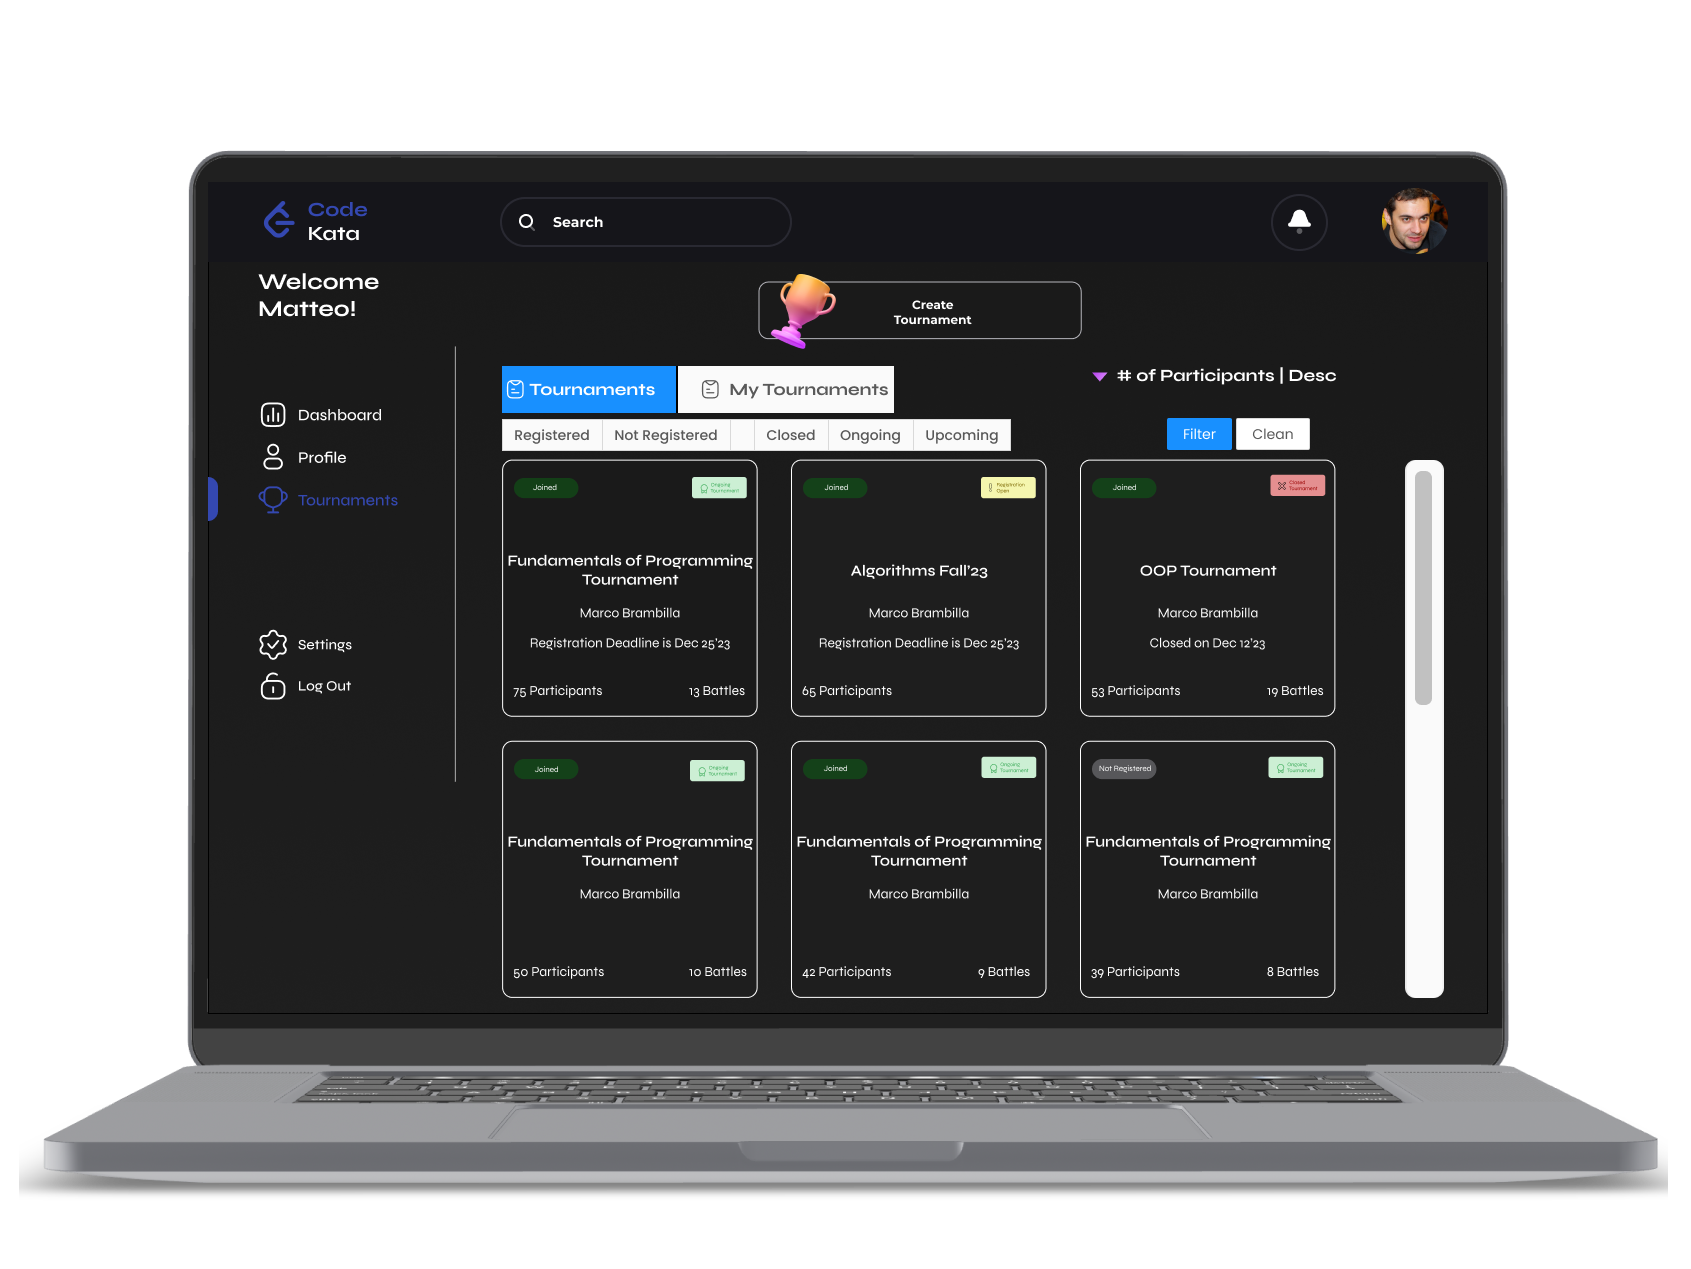
\includegraphics[scale=0.13]{Images/ui-ux/educator_tournaments/educator_tournaments_1.png}
% 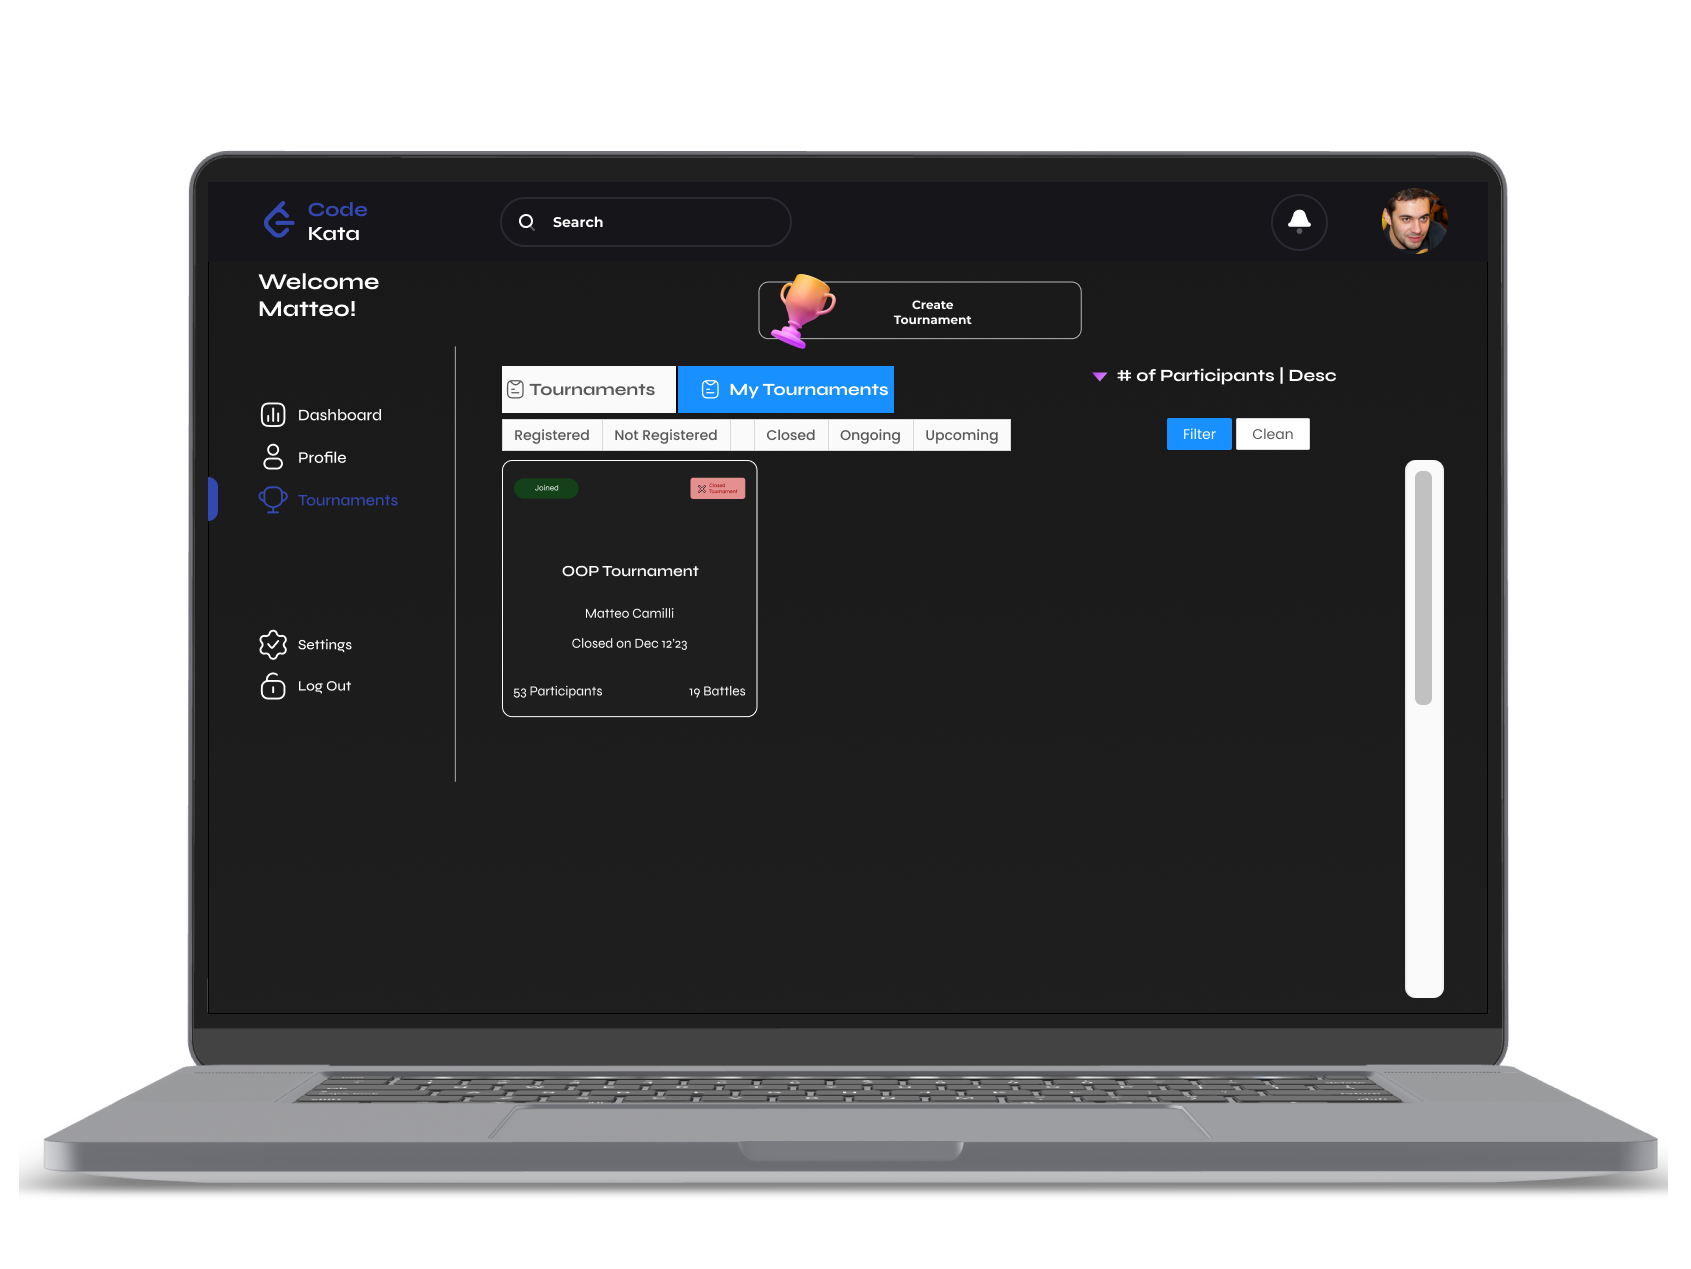
\includegraphics[scale=0.13]{Images/ui-ux/educator_tournaments/educator_tournaments_2.png}
%         (a) Educator Tournaments
% \end{center}
% \begin{center}
% 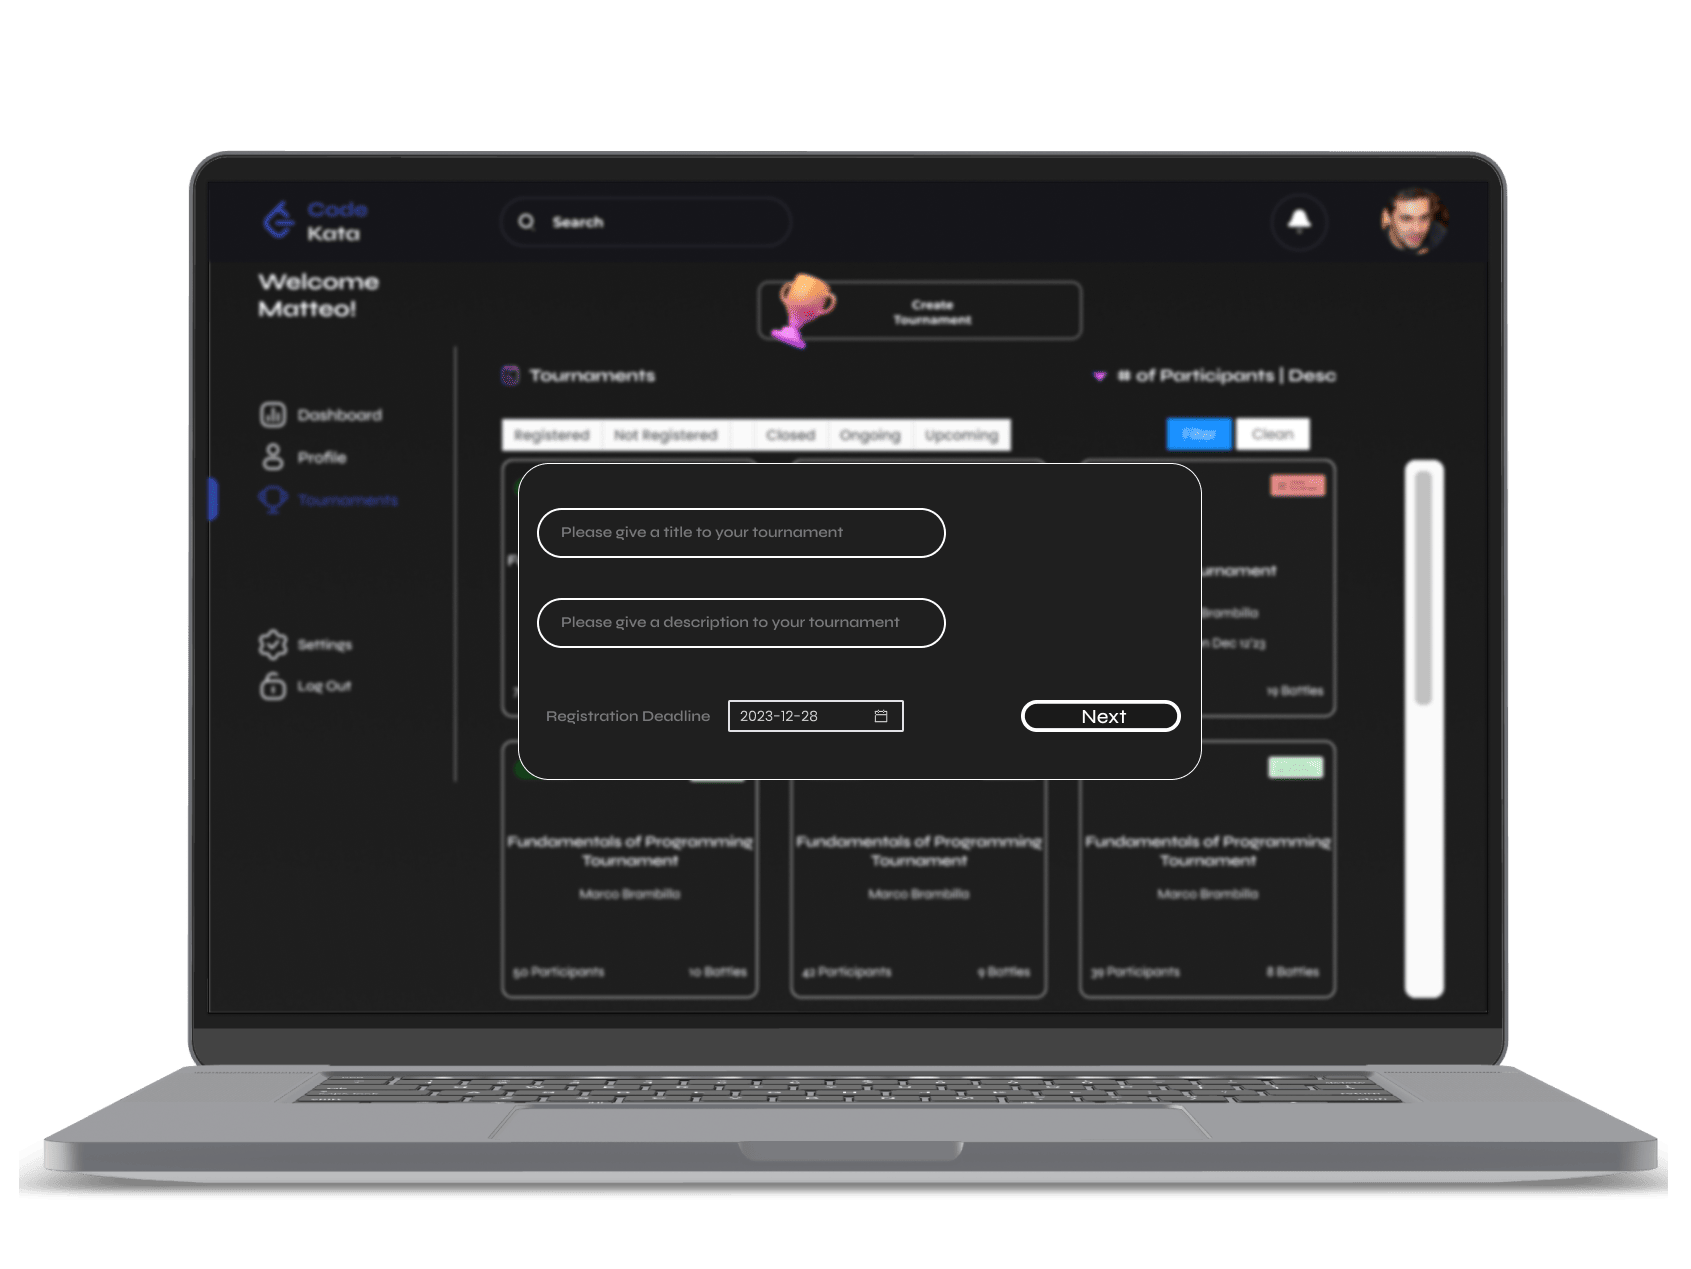
\includegraphics[scale=0.13]{Images/ui-ux/educator_create_tournament/educator_create_tournament_1.png}
% 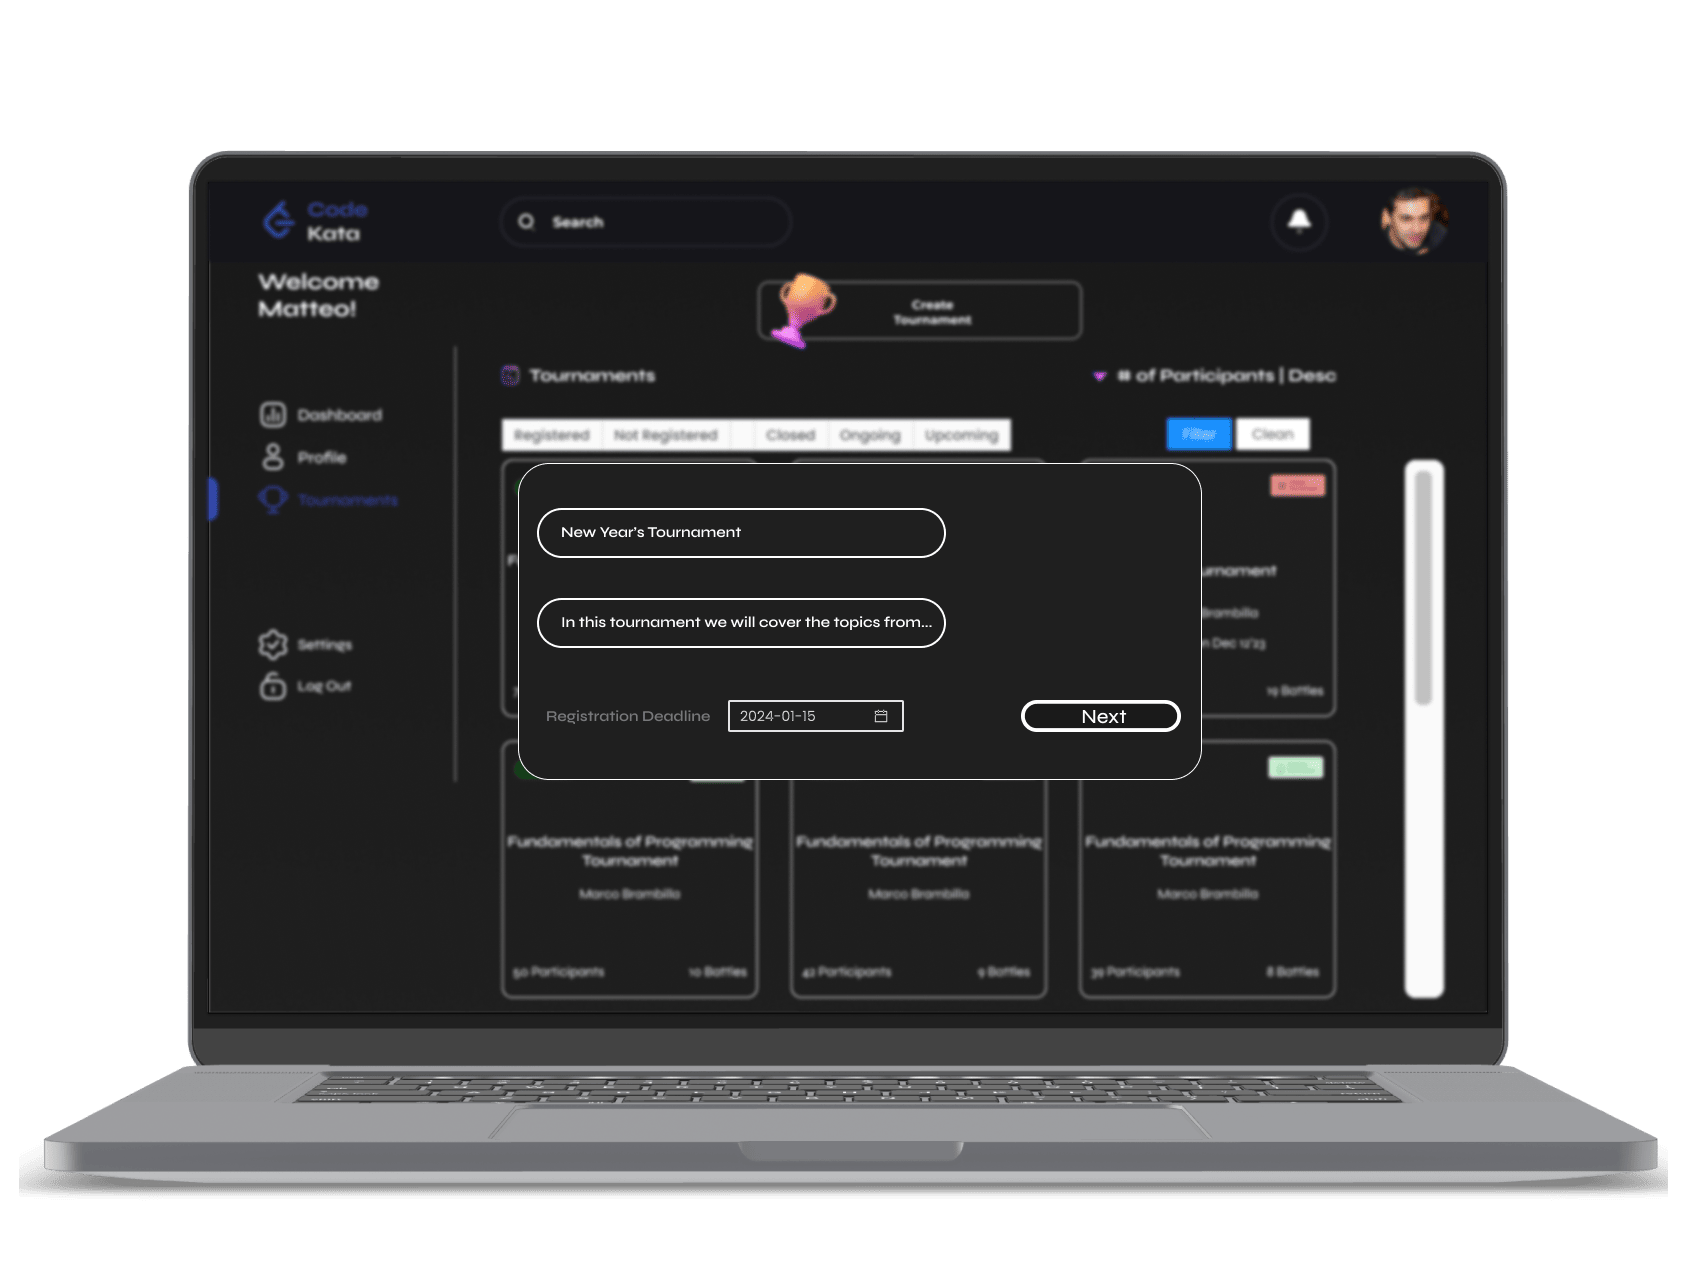
\includegraphics[scale=0.13]{Images/ui-ux/educator_create_tournament/educator_create_tournament_2.png}
% 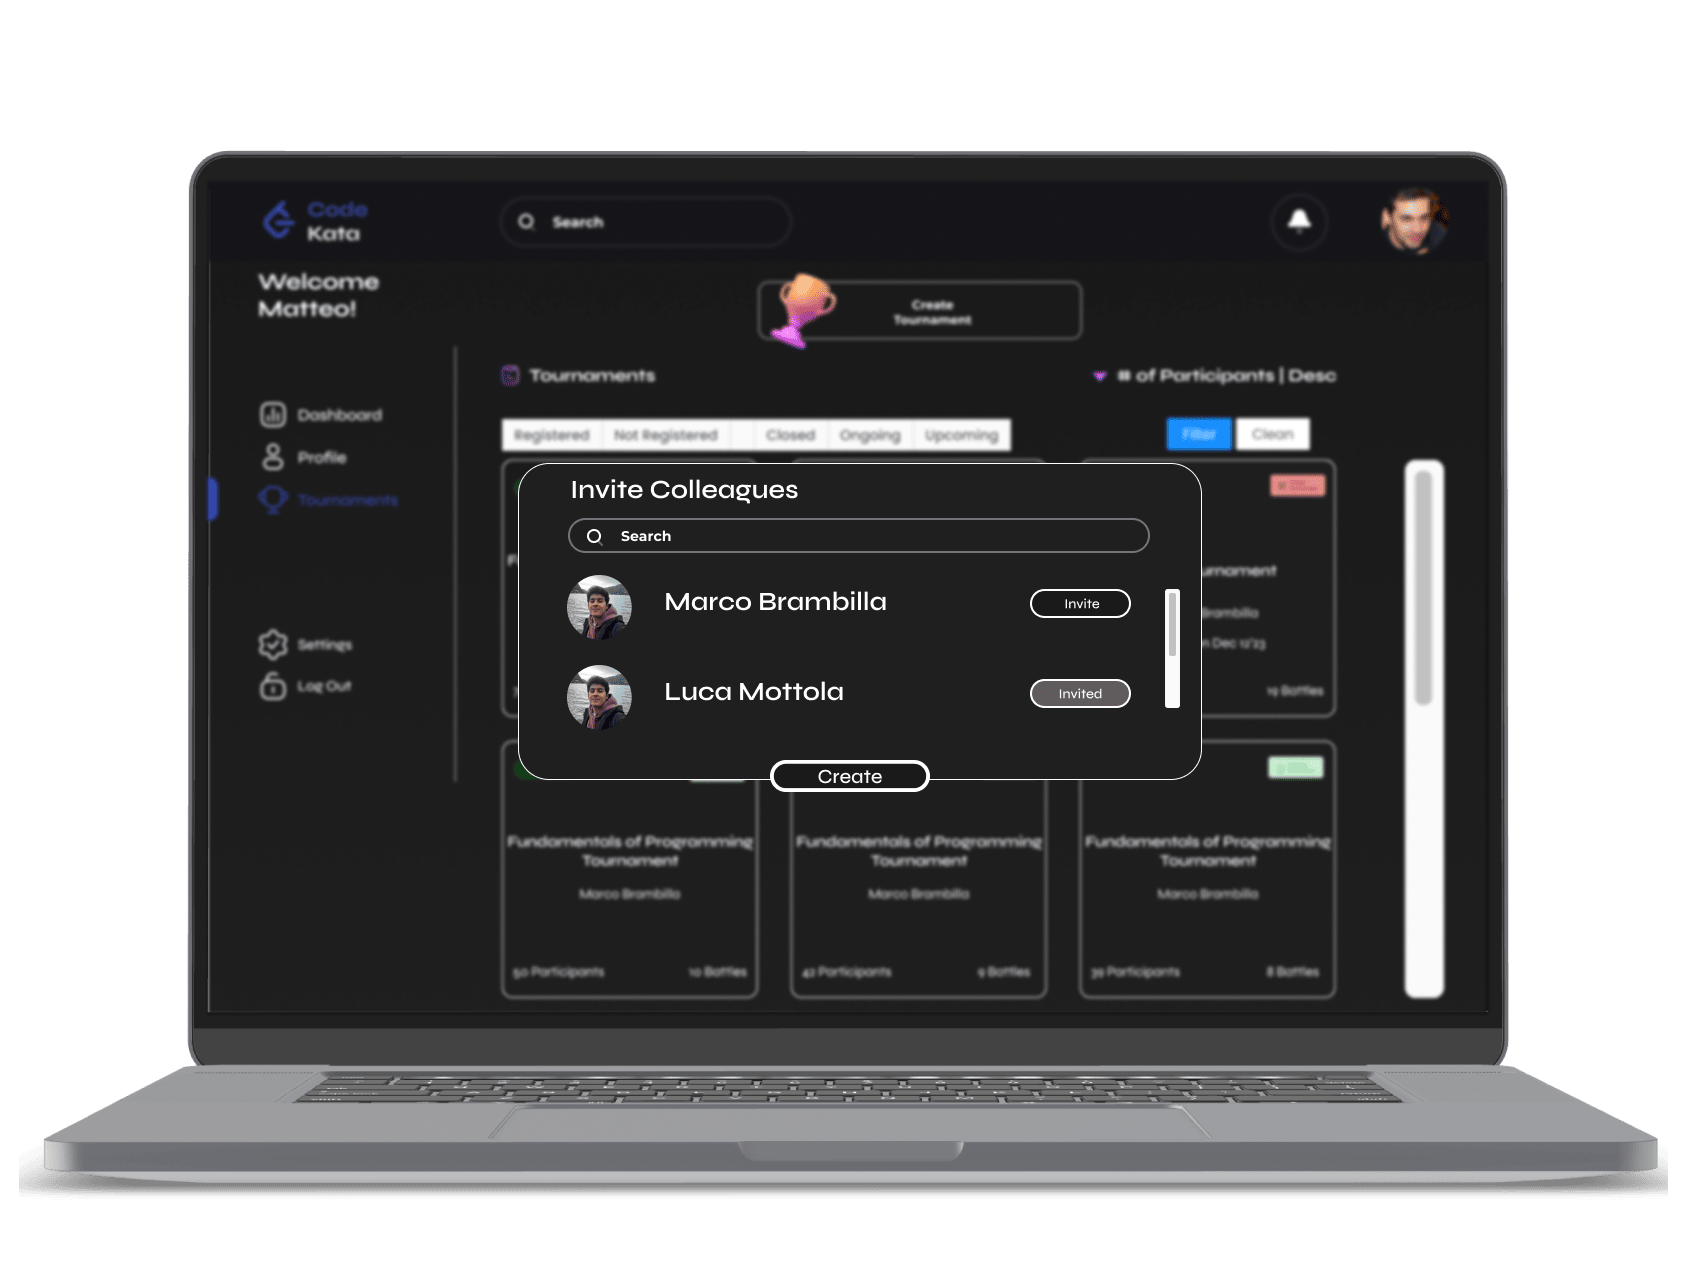
\includegraphics[scale=0.13]{Images/ui-ux/educator_create_tournament/educator_create_tournament_3.png}
% 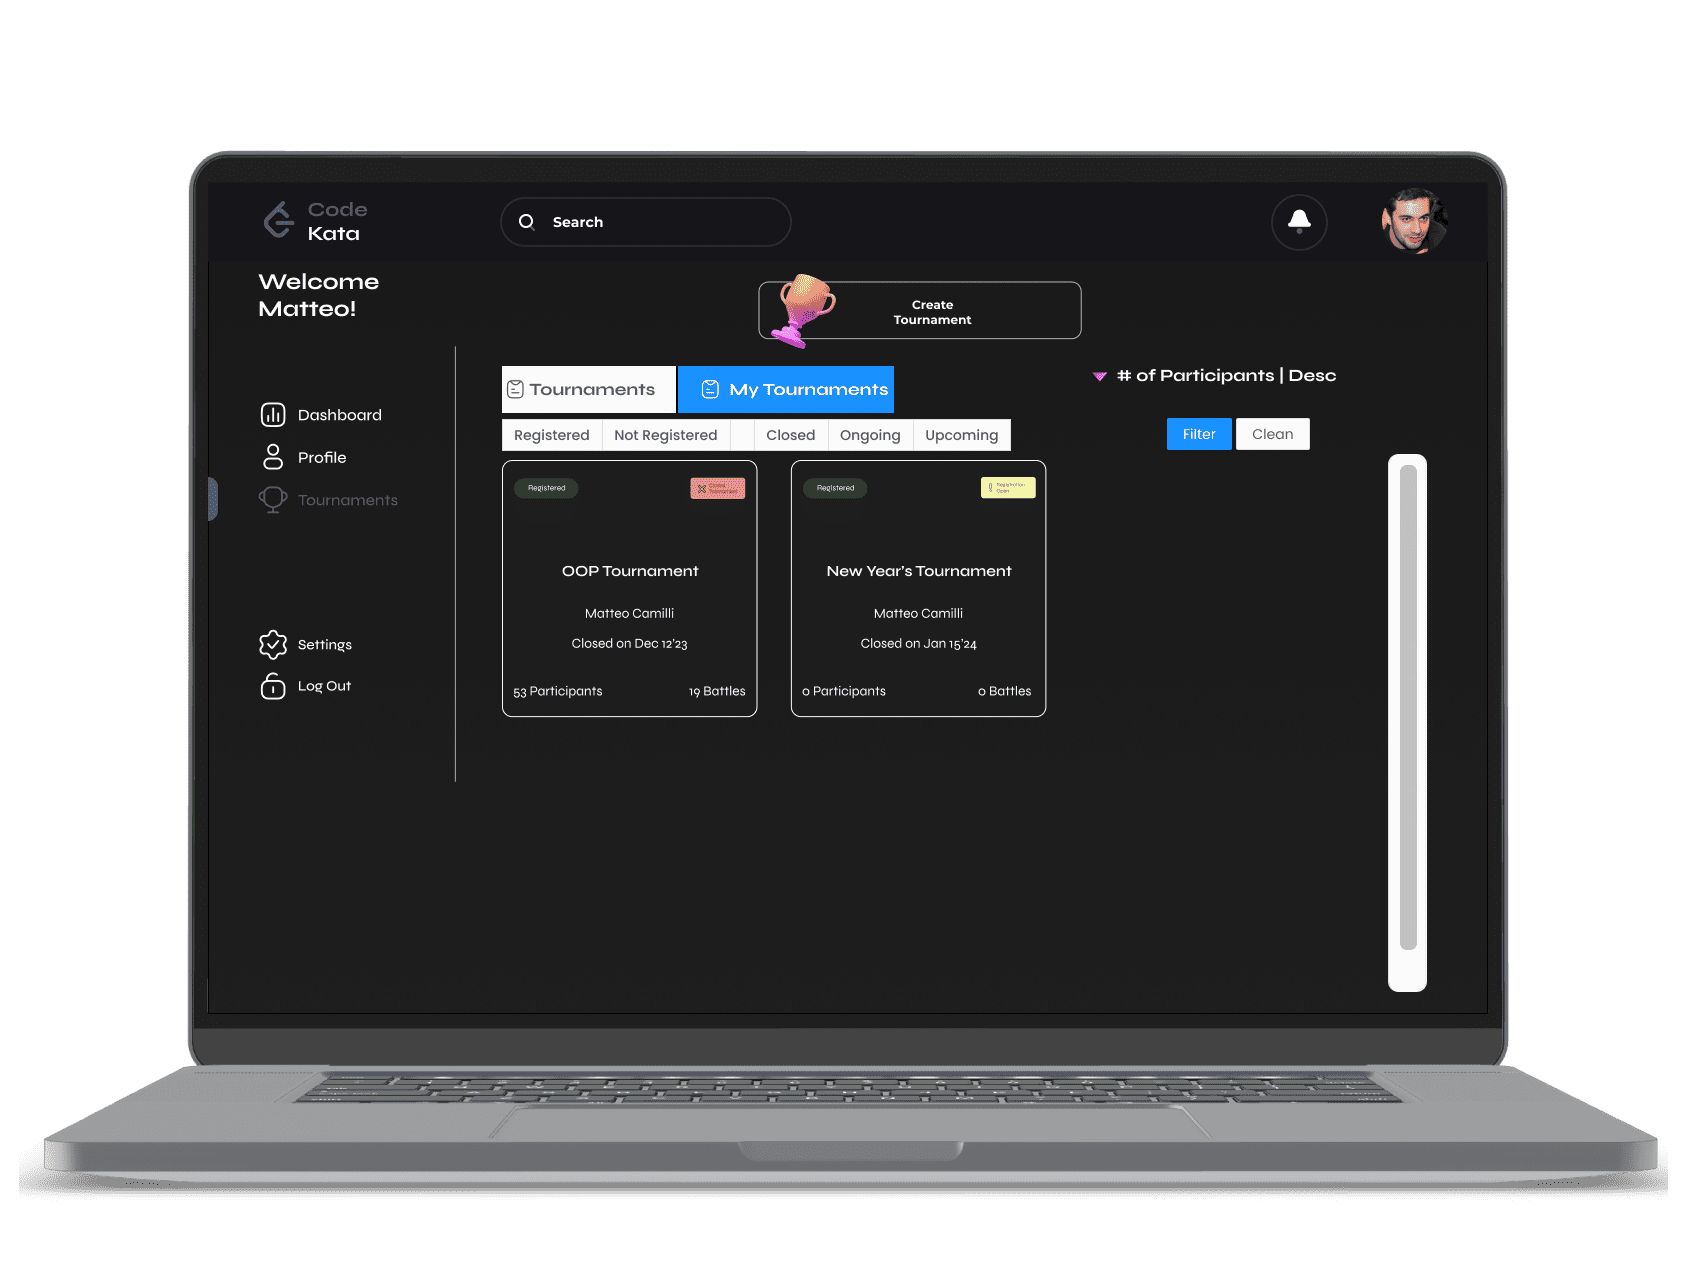
\includegraphics[scale=0.13]{Images/ui-ux/educator_create_tournament/educator_create_tournament_4.png}
%         (a) Educator Creates Tournaments
% \end{center}
% \begin{center}
% 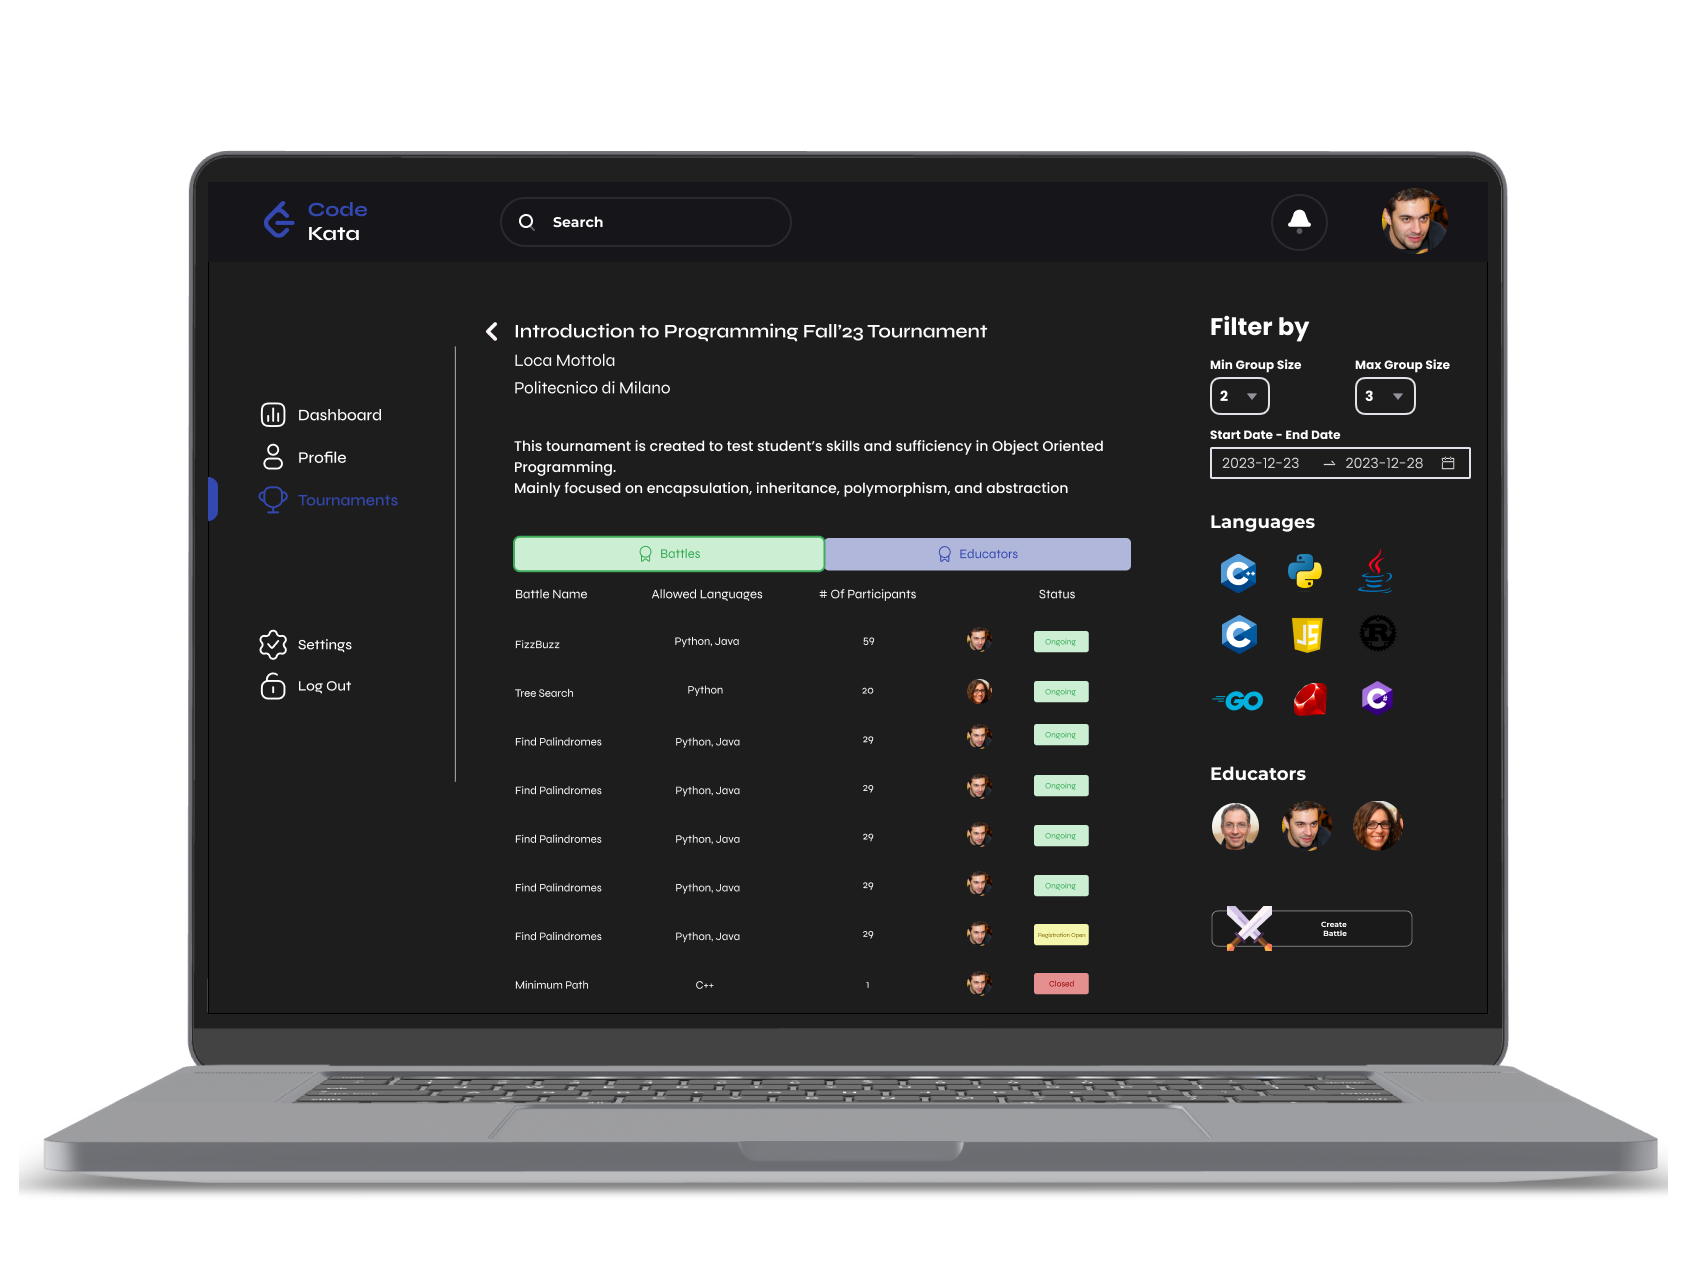
\includegraphics[scale=0.13]{Images/ui-ux/educator_creates_battle/educator_creates_battle_1.png}
% 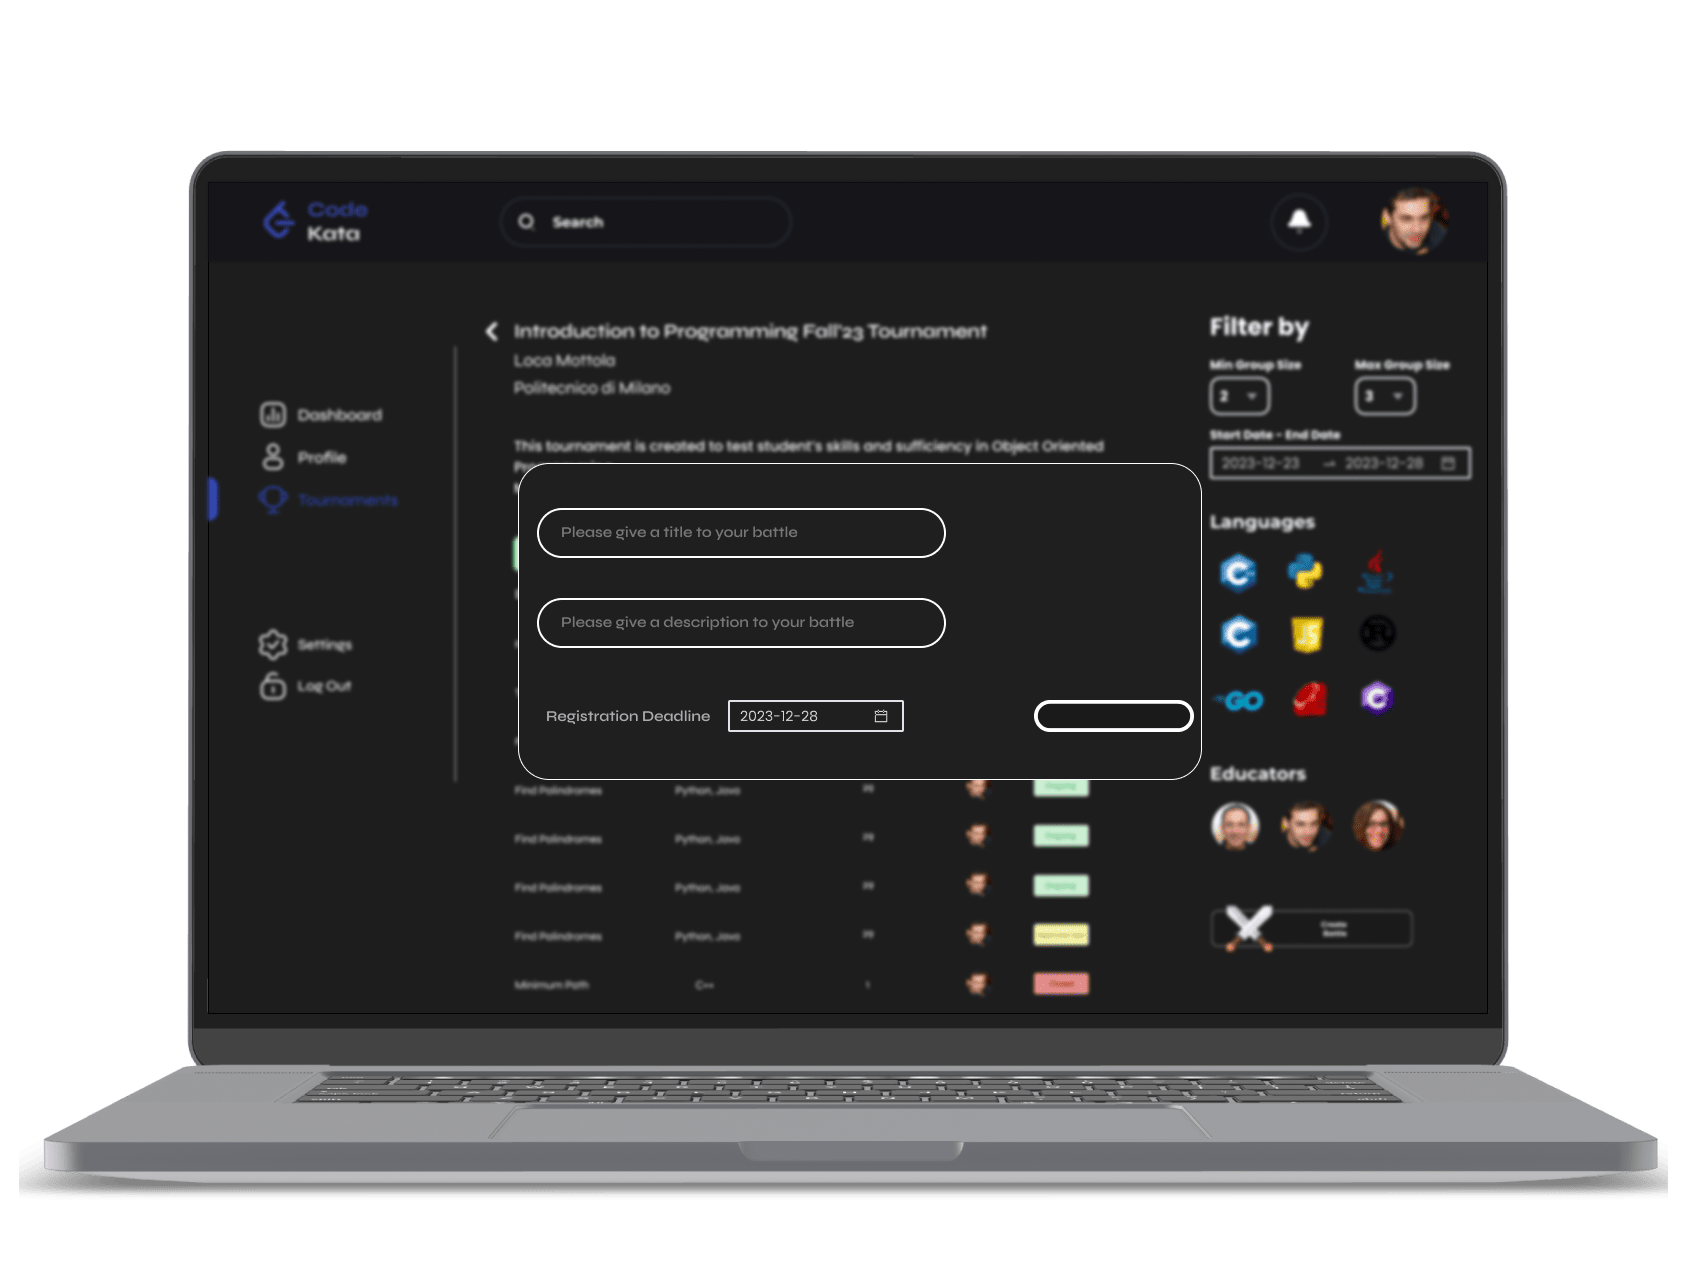
\includegraphics[scale=0.13]{Images/ui-ux/educator_creates_battle/educator_creates_battle_2.png}
% 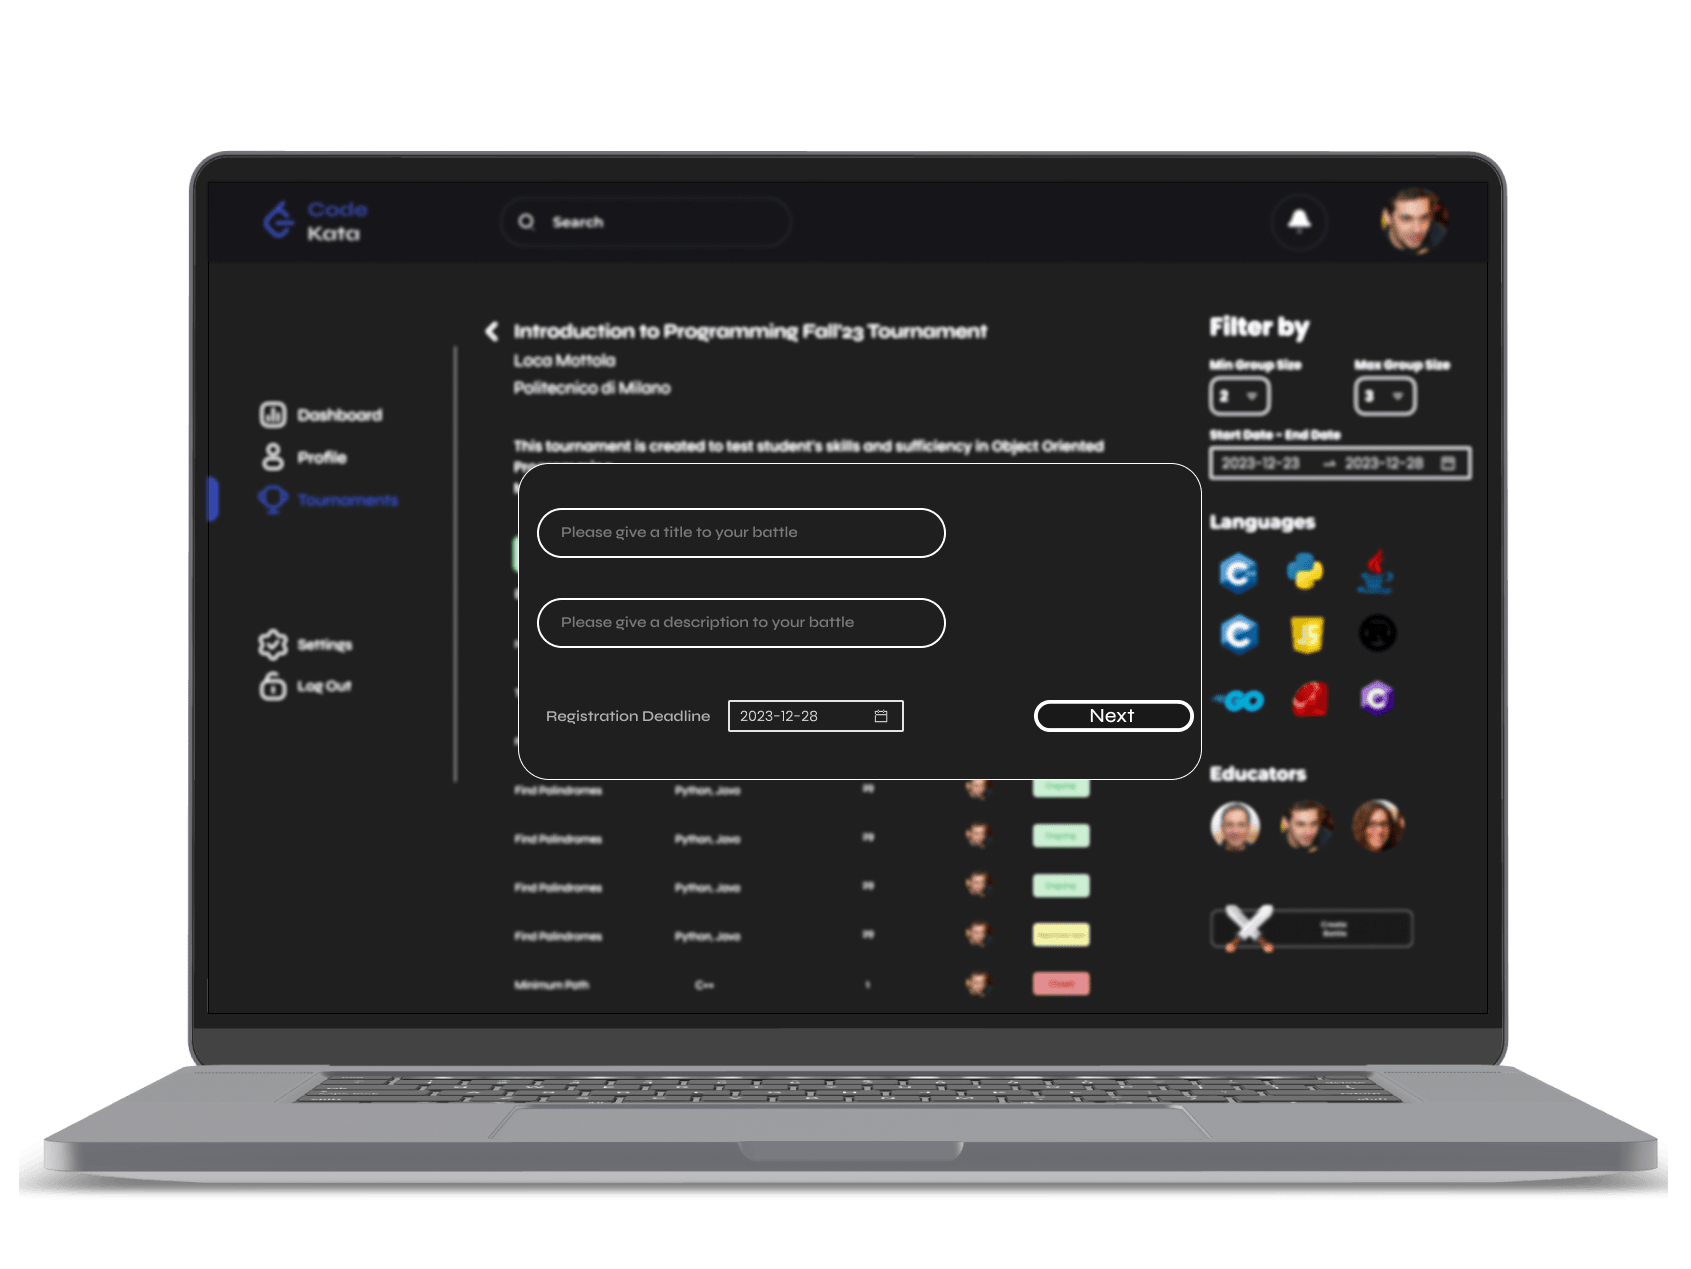
\includegraphics[scale=0.13]{Images/ui-ux/educator_creates_battle/educator_creates_battle_3.png}
% 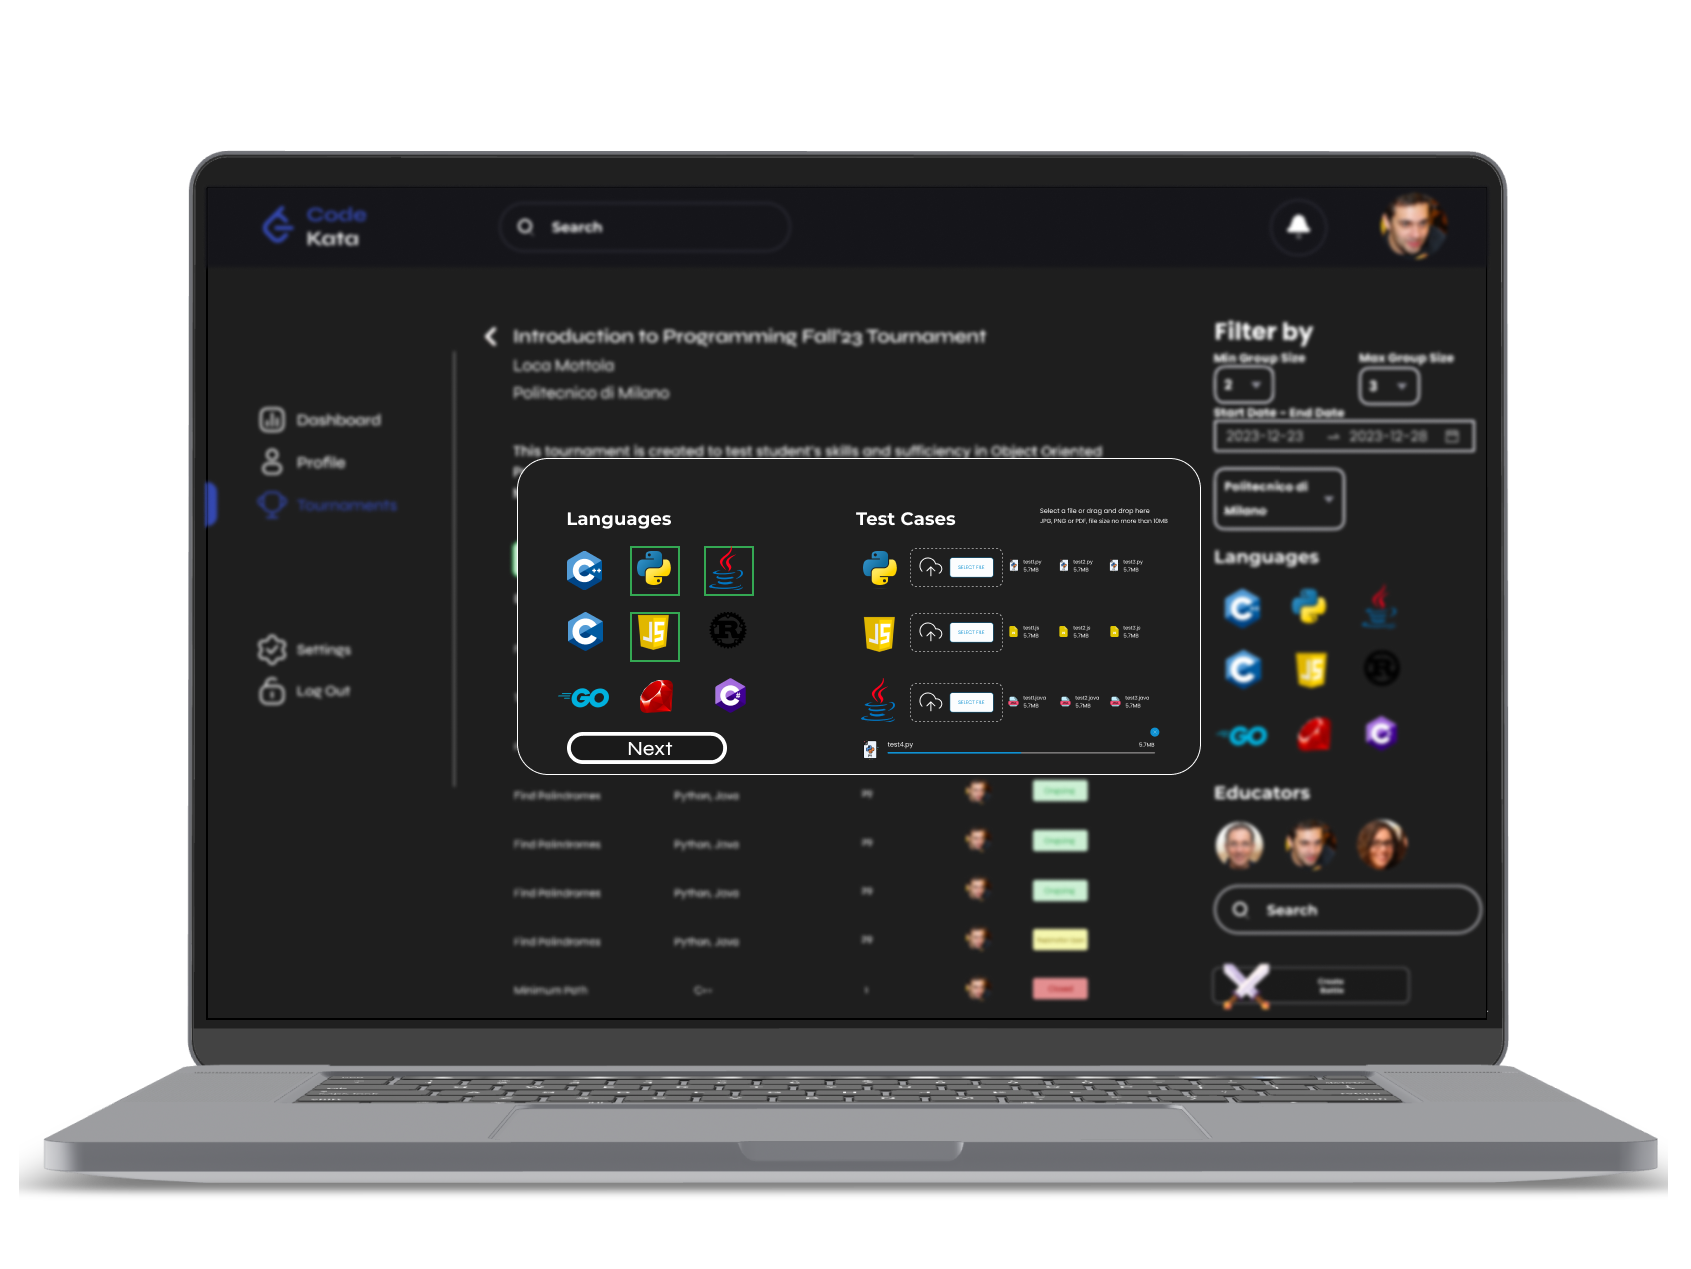
\includegraphics[scale=0.13]{Images/ui-ux/educator_creates_battle/educator_creates_battle_4.png}
% 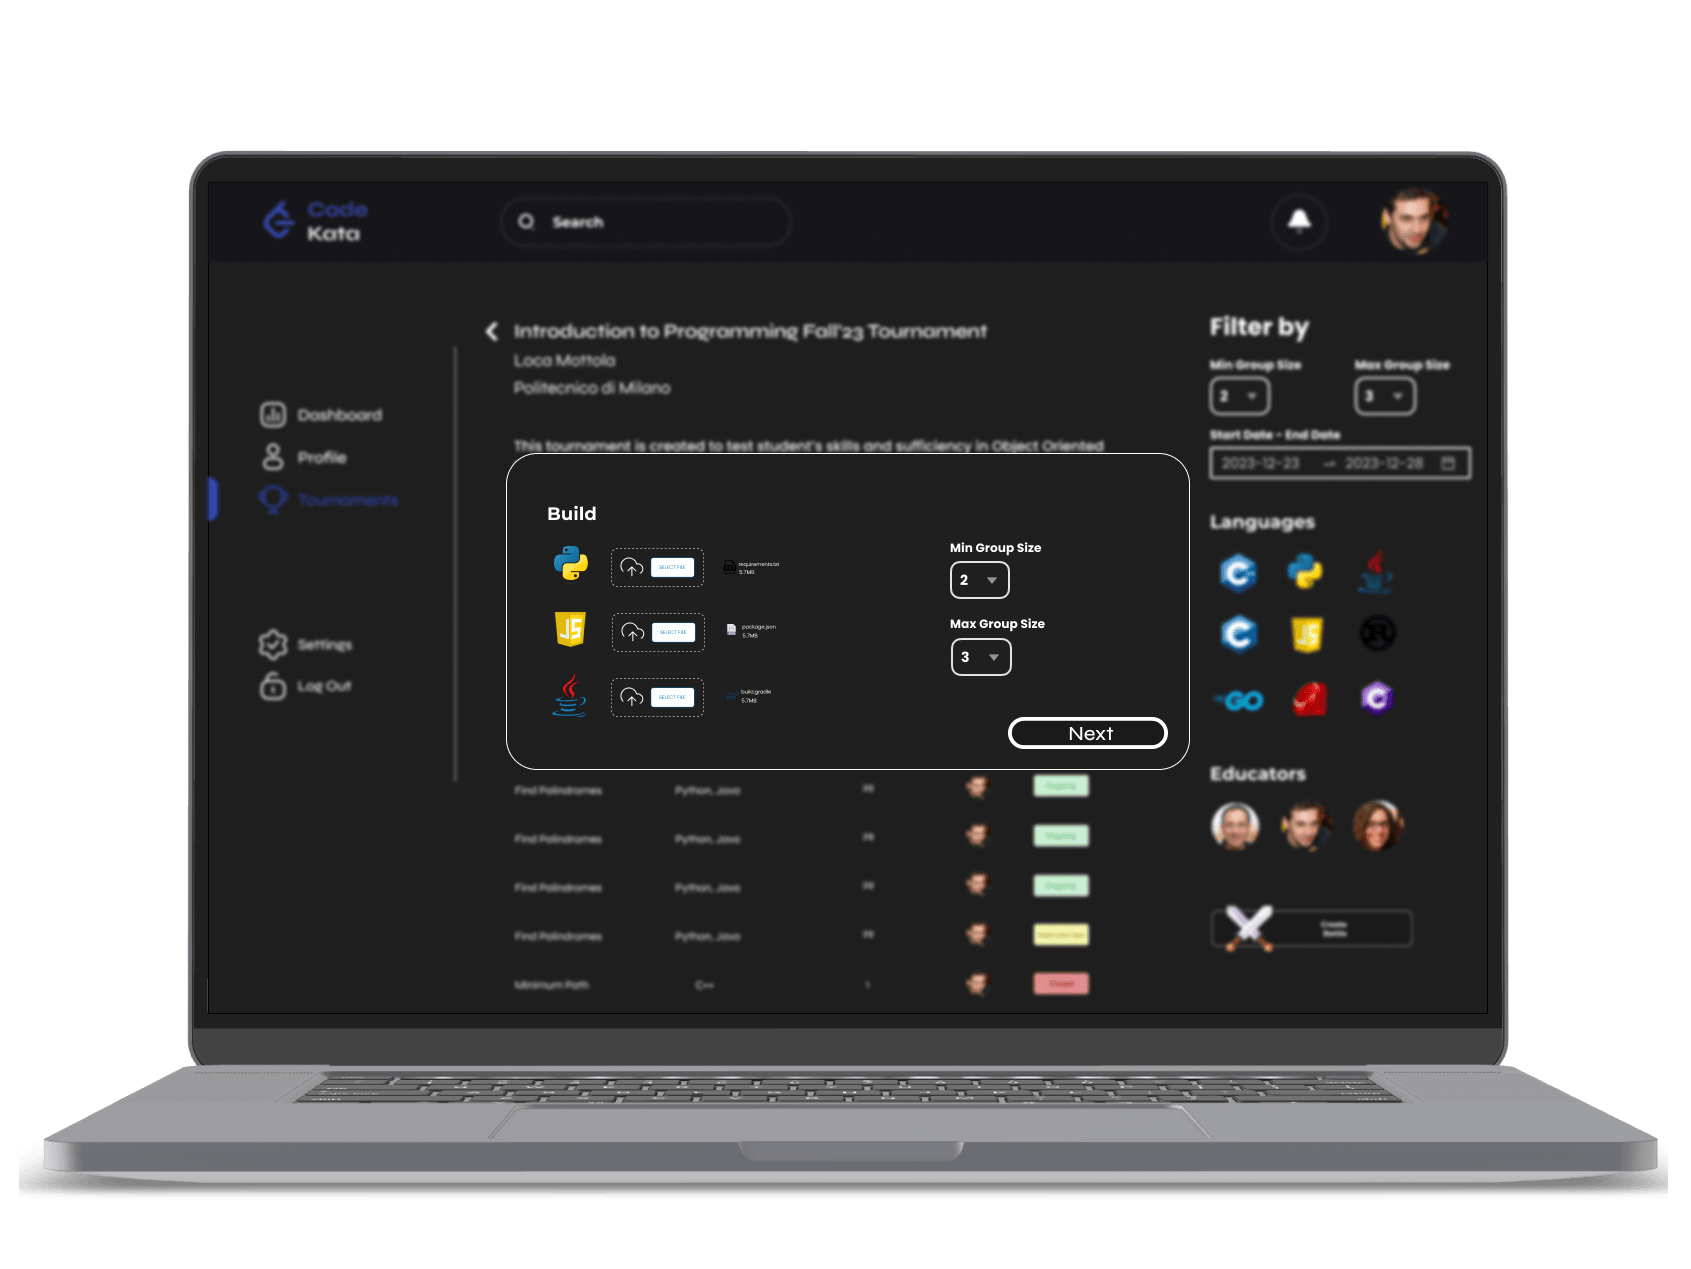
\includegraphics[scale=0.13]{Images/ui-ux/educator_creates_battle/educator_creates_battle_5.png}
% 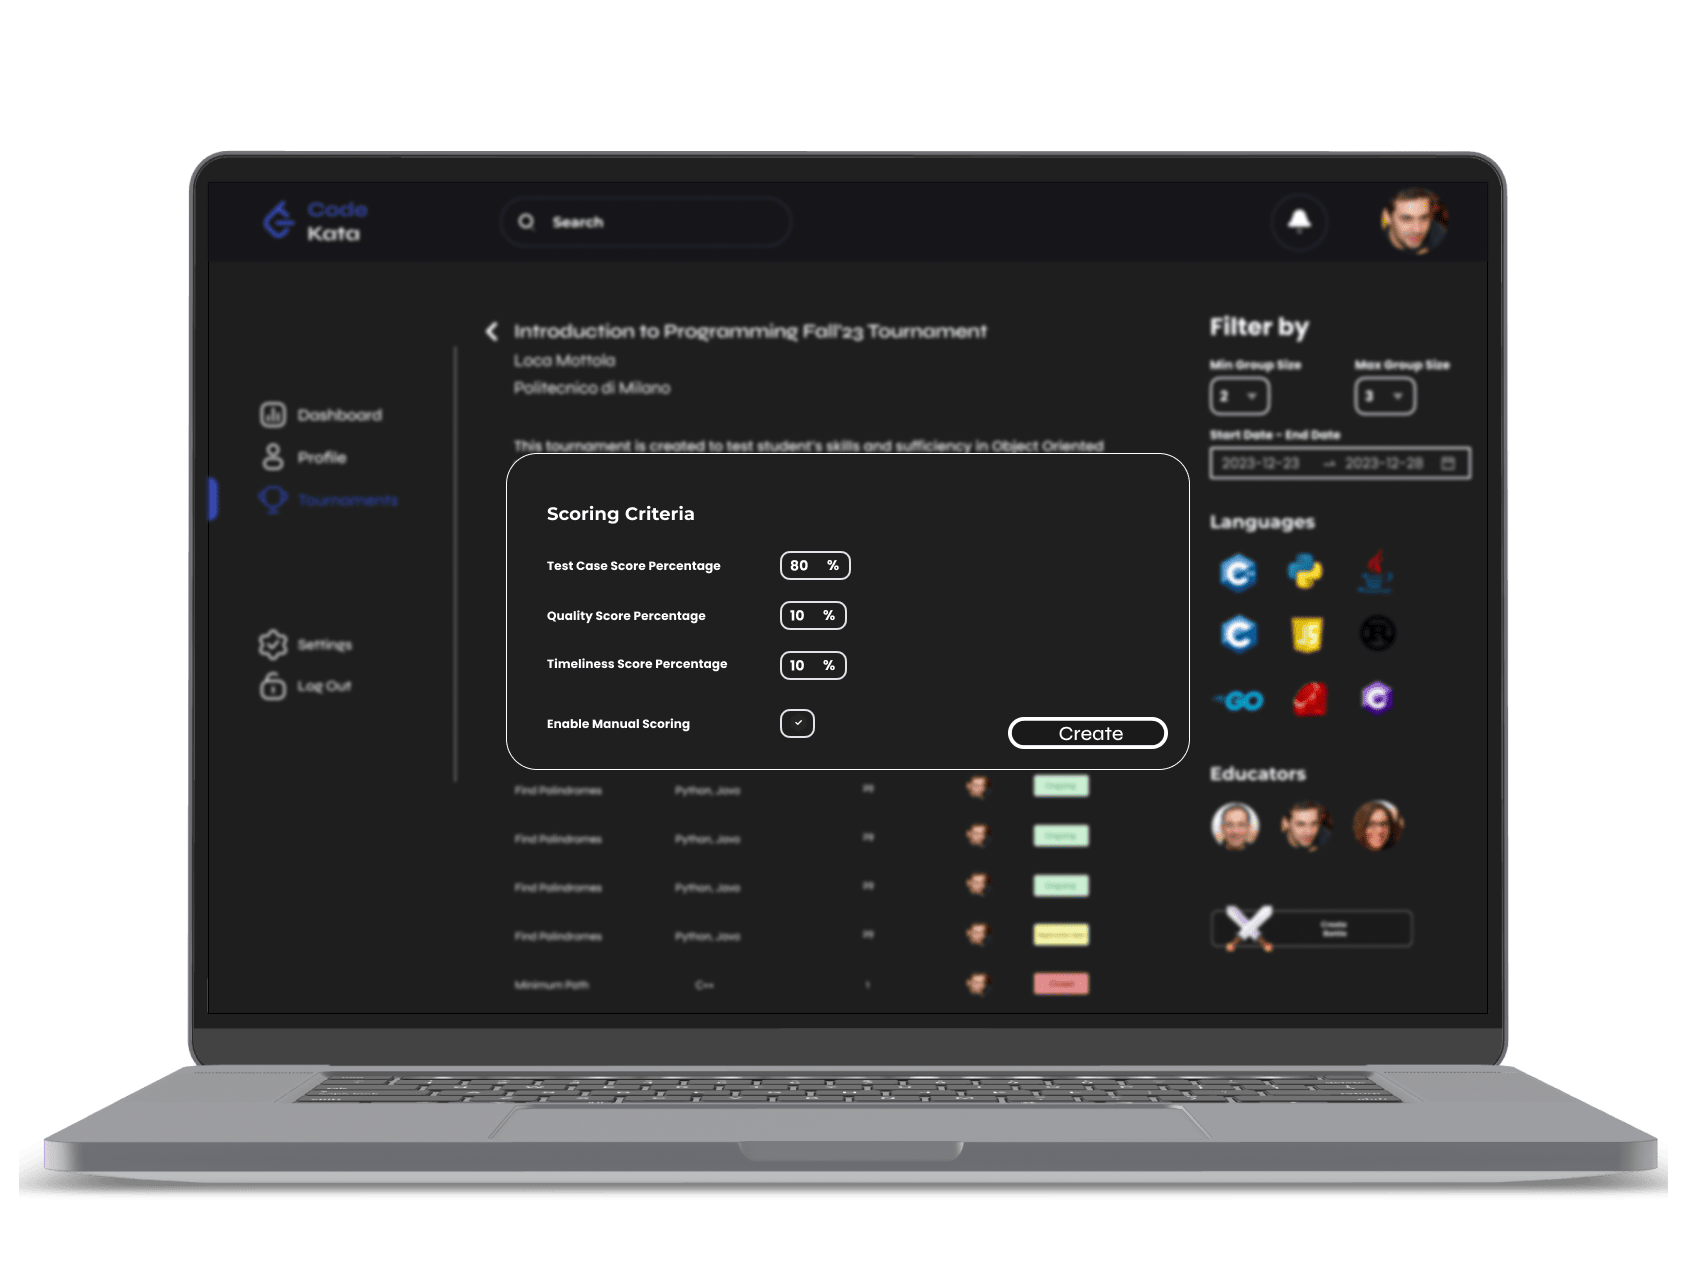
\includegraphics[scale=0.13]{Images/ui-ux/educator_creates_battle/educator_creates_battle_6.png}
%         (a) Educator Creates Battle
% \end{center}
% \begin{center}
% 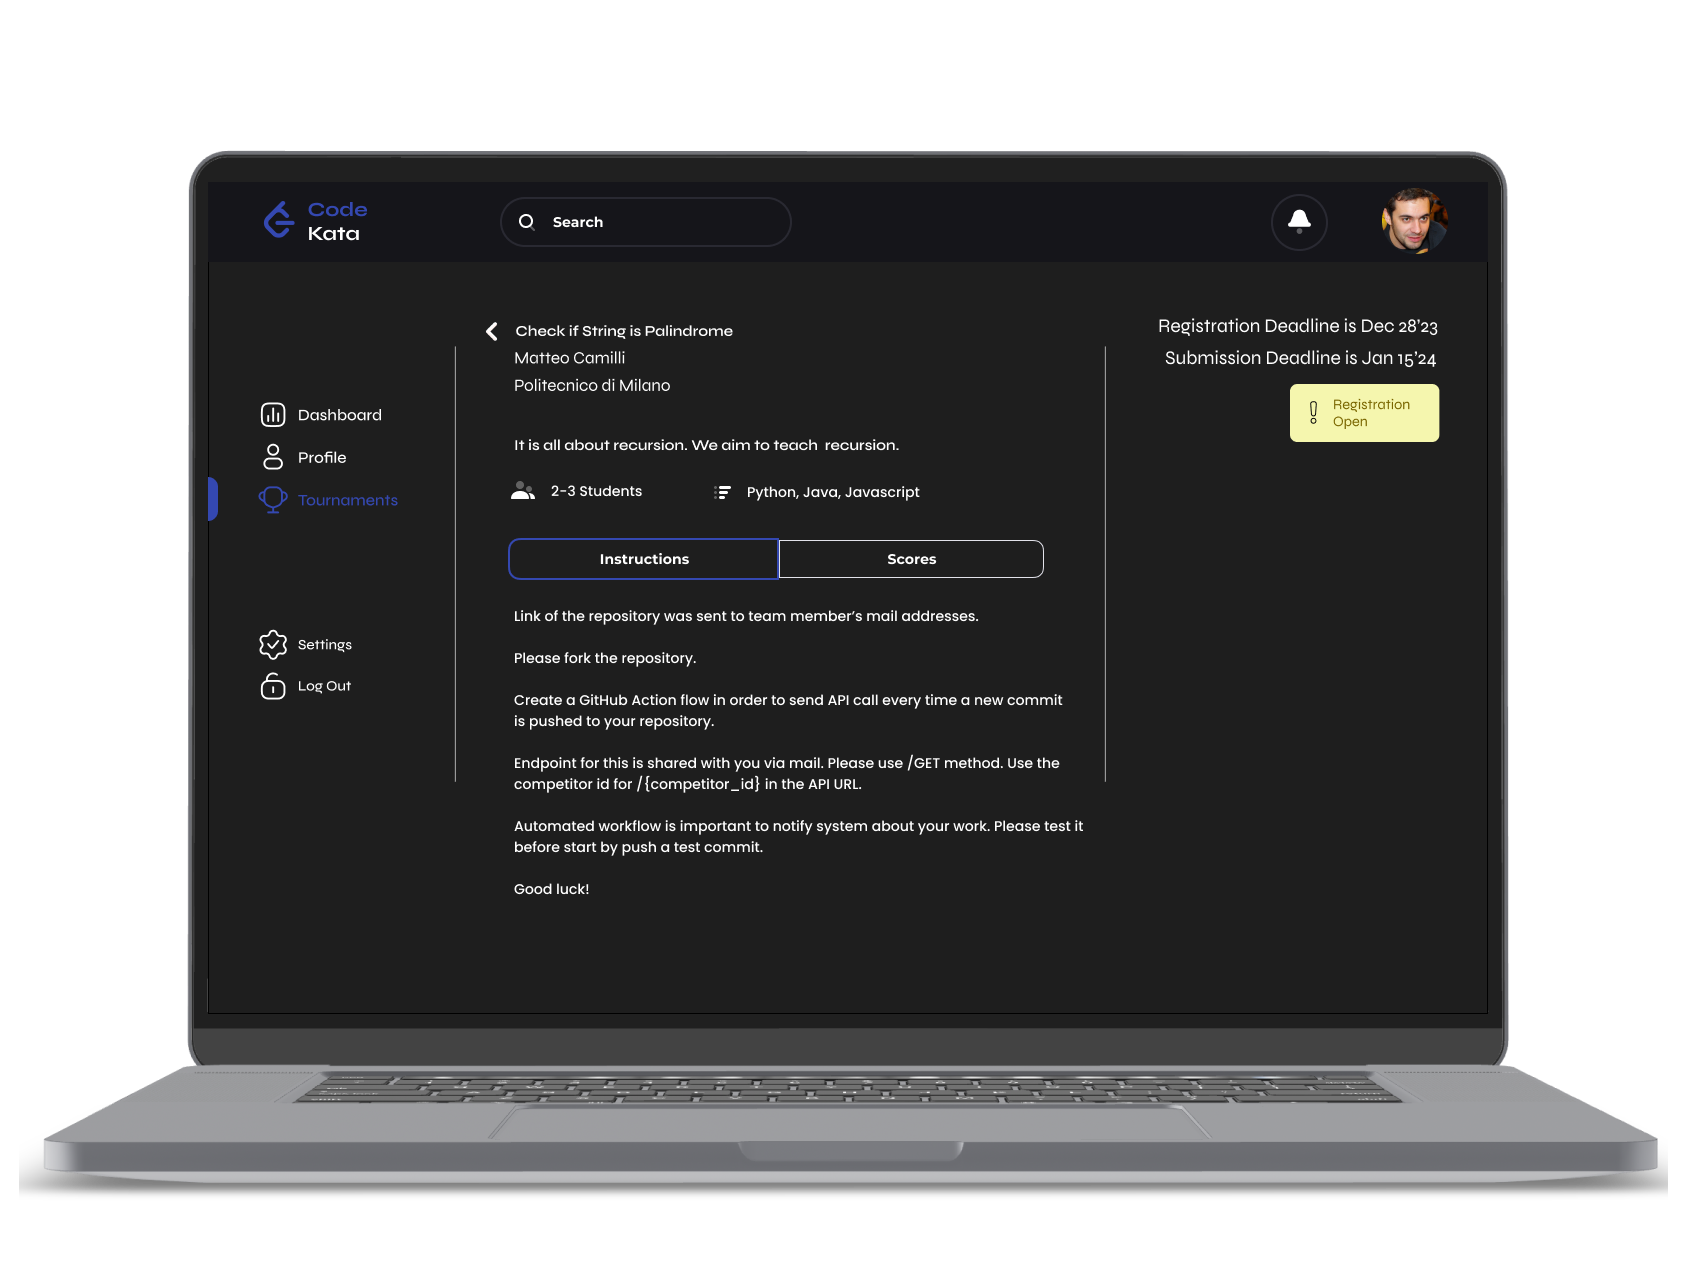
\includegraphics[scale=0.13]{Images/ui-ux/educator_battle/educator_battle_1.png}
% 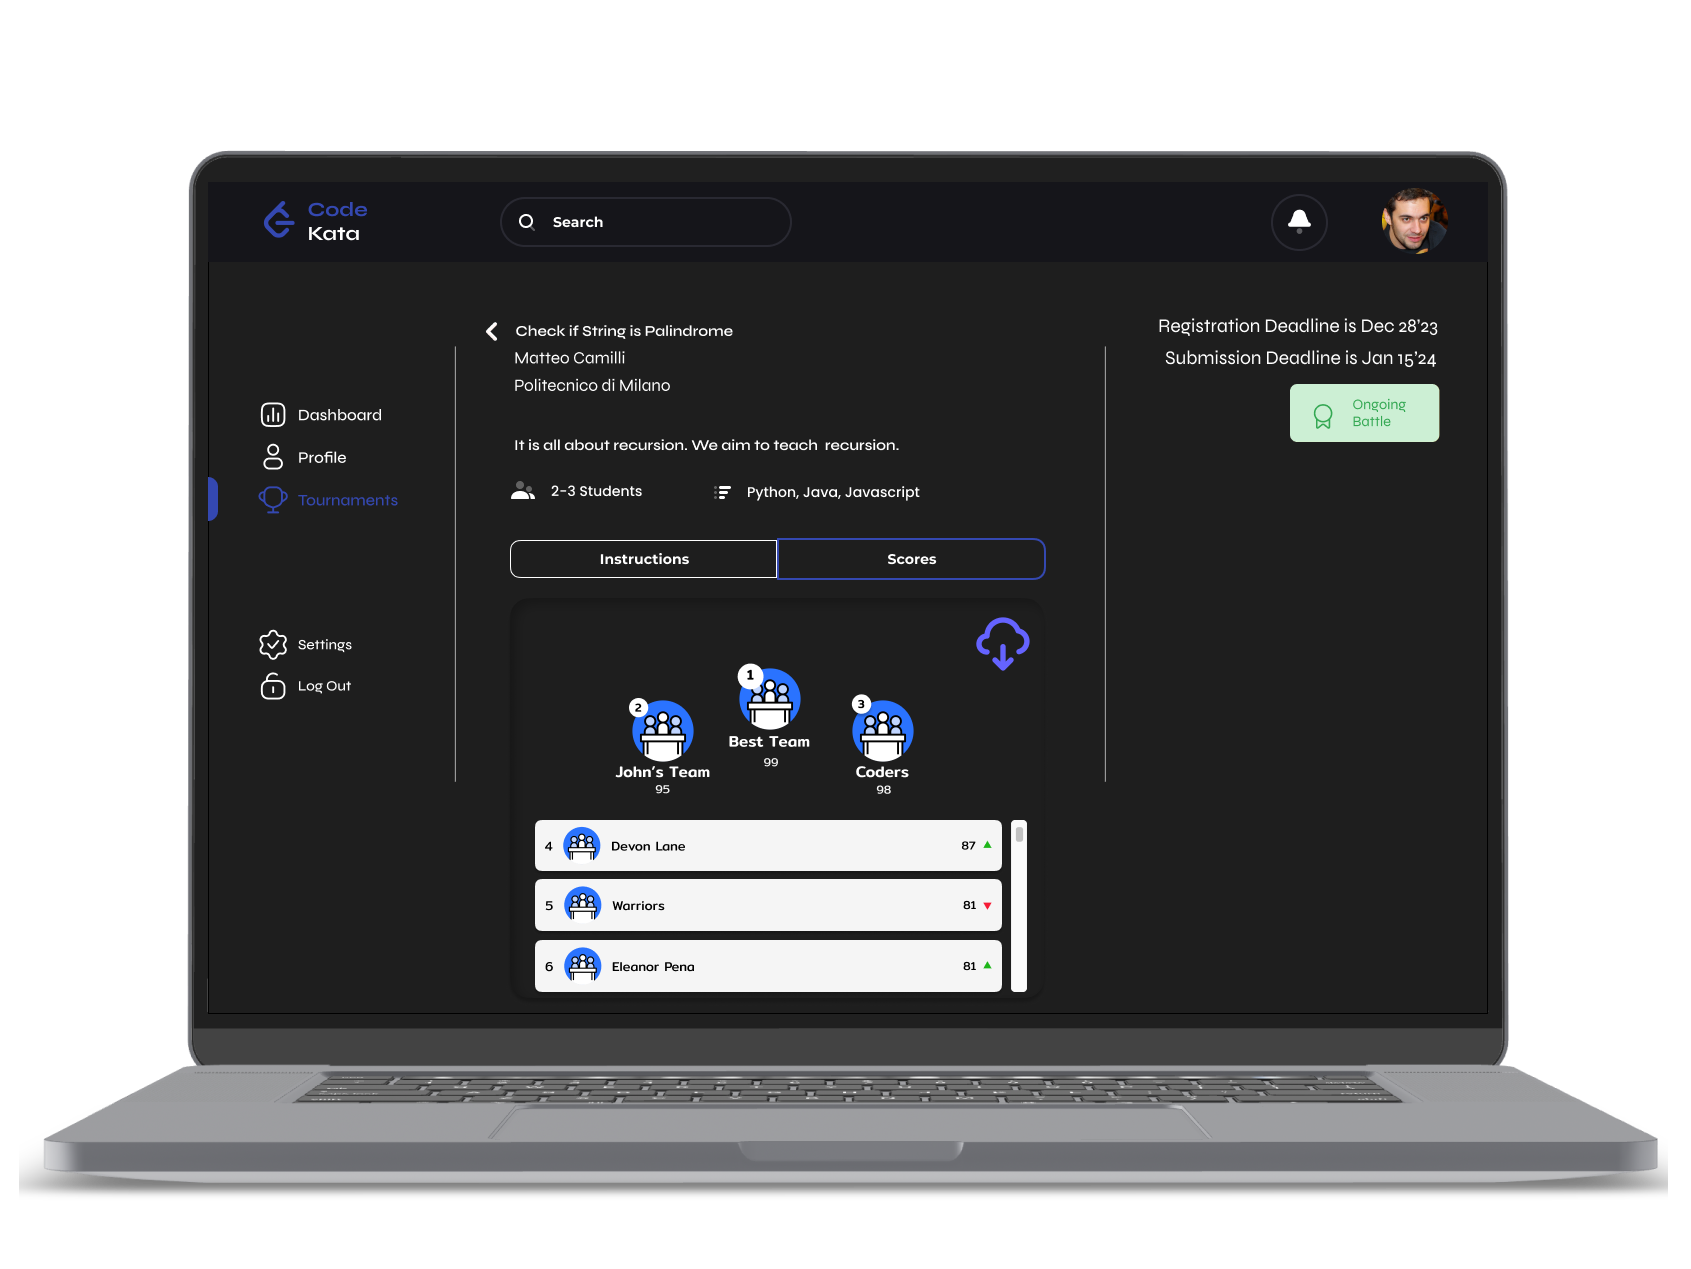
\includegraphics[scale=0.13]{Images/ui-ux/educator_battle/educator_battle_2.png}
% 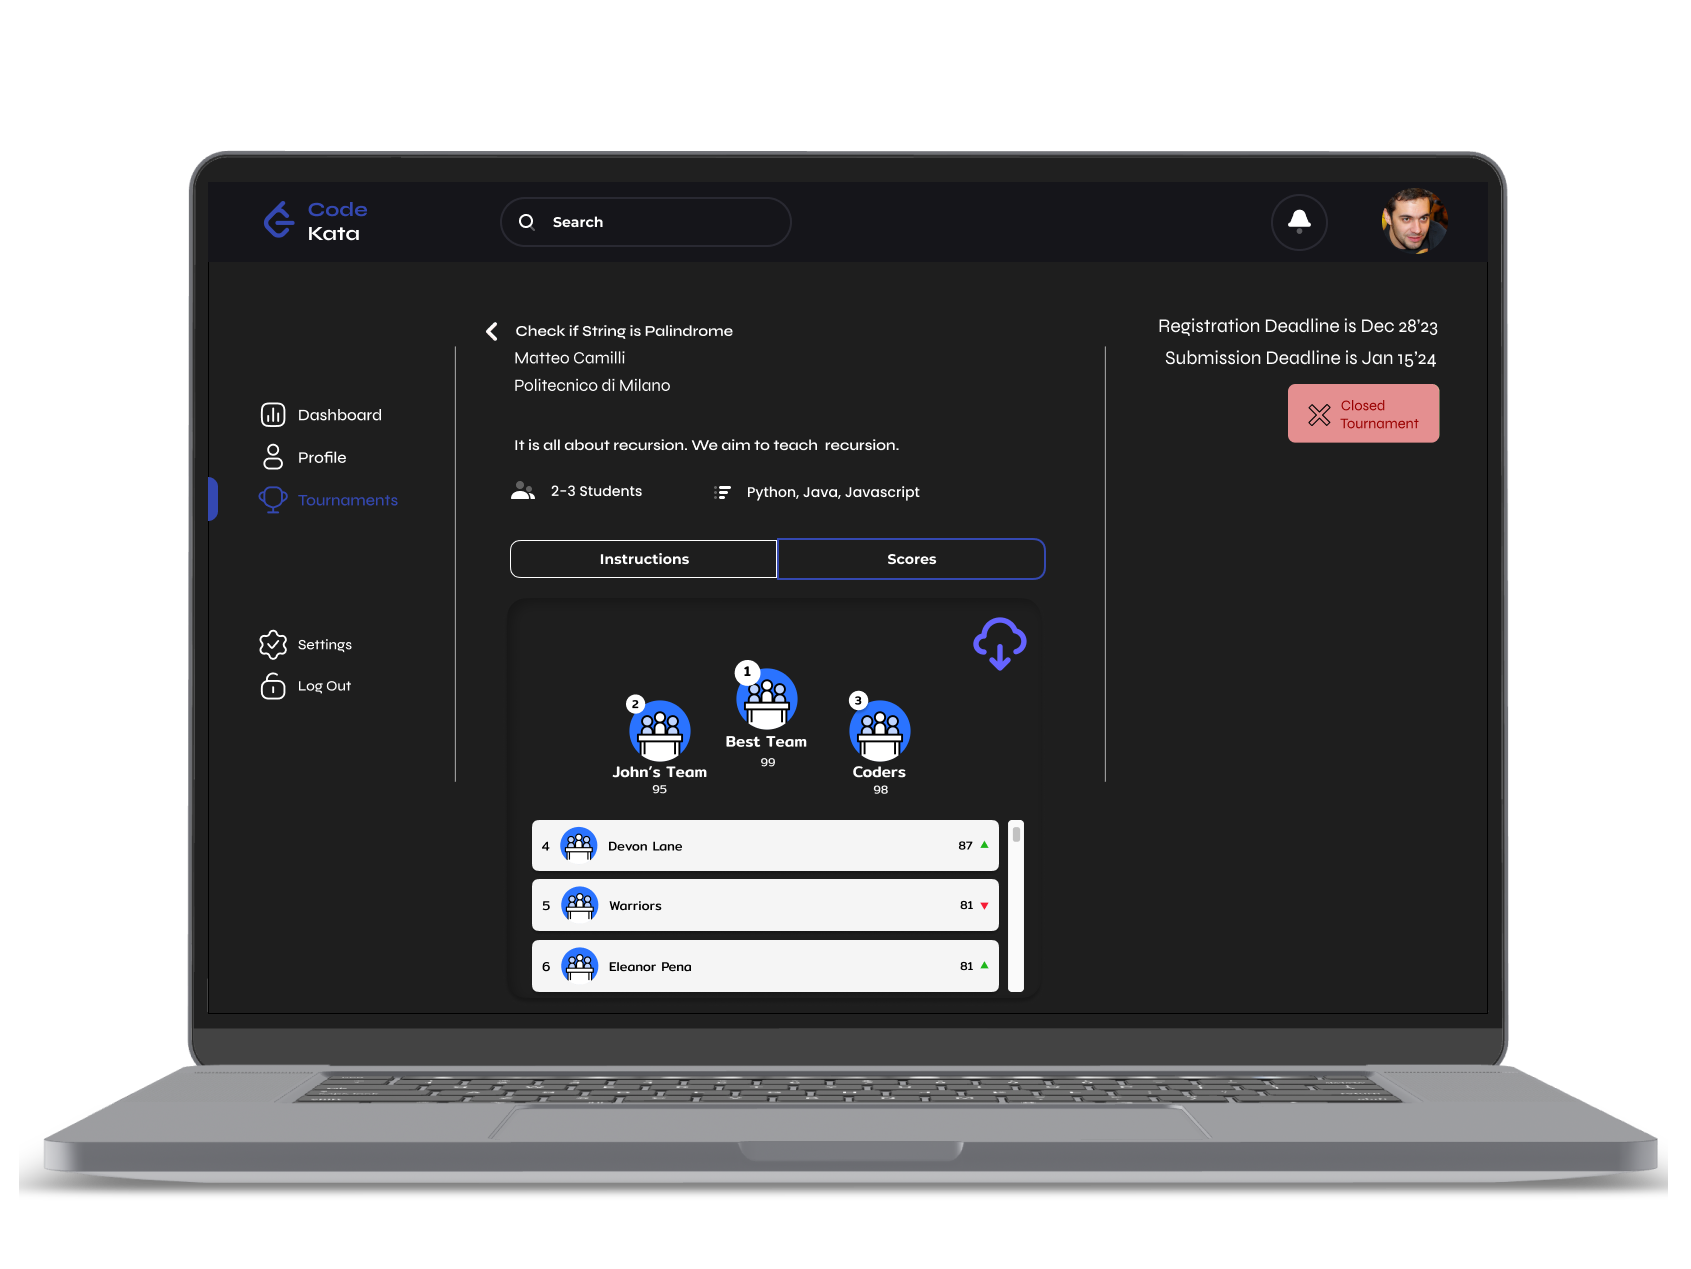
\includegraphics[scale=0.13]{Images/ui-ux/educator_battle/educator_battle_3.png}
%  \\(a) Educator and Battle
% \end{center}
% \begin{center}
% 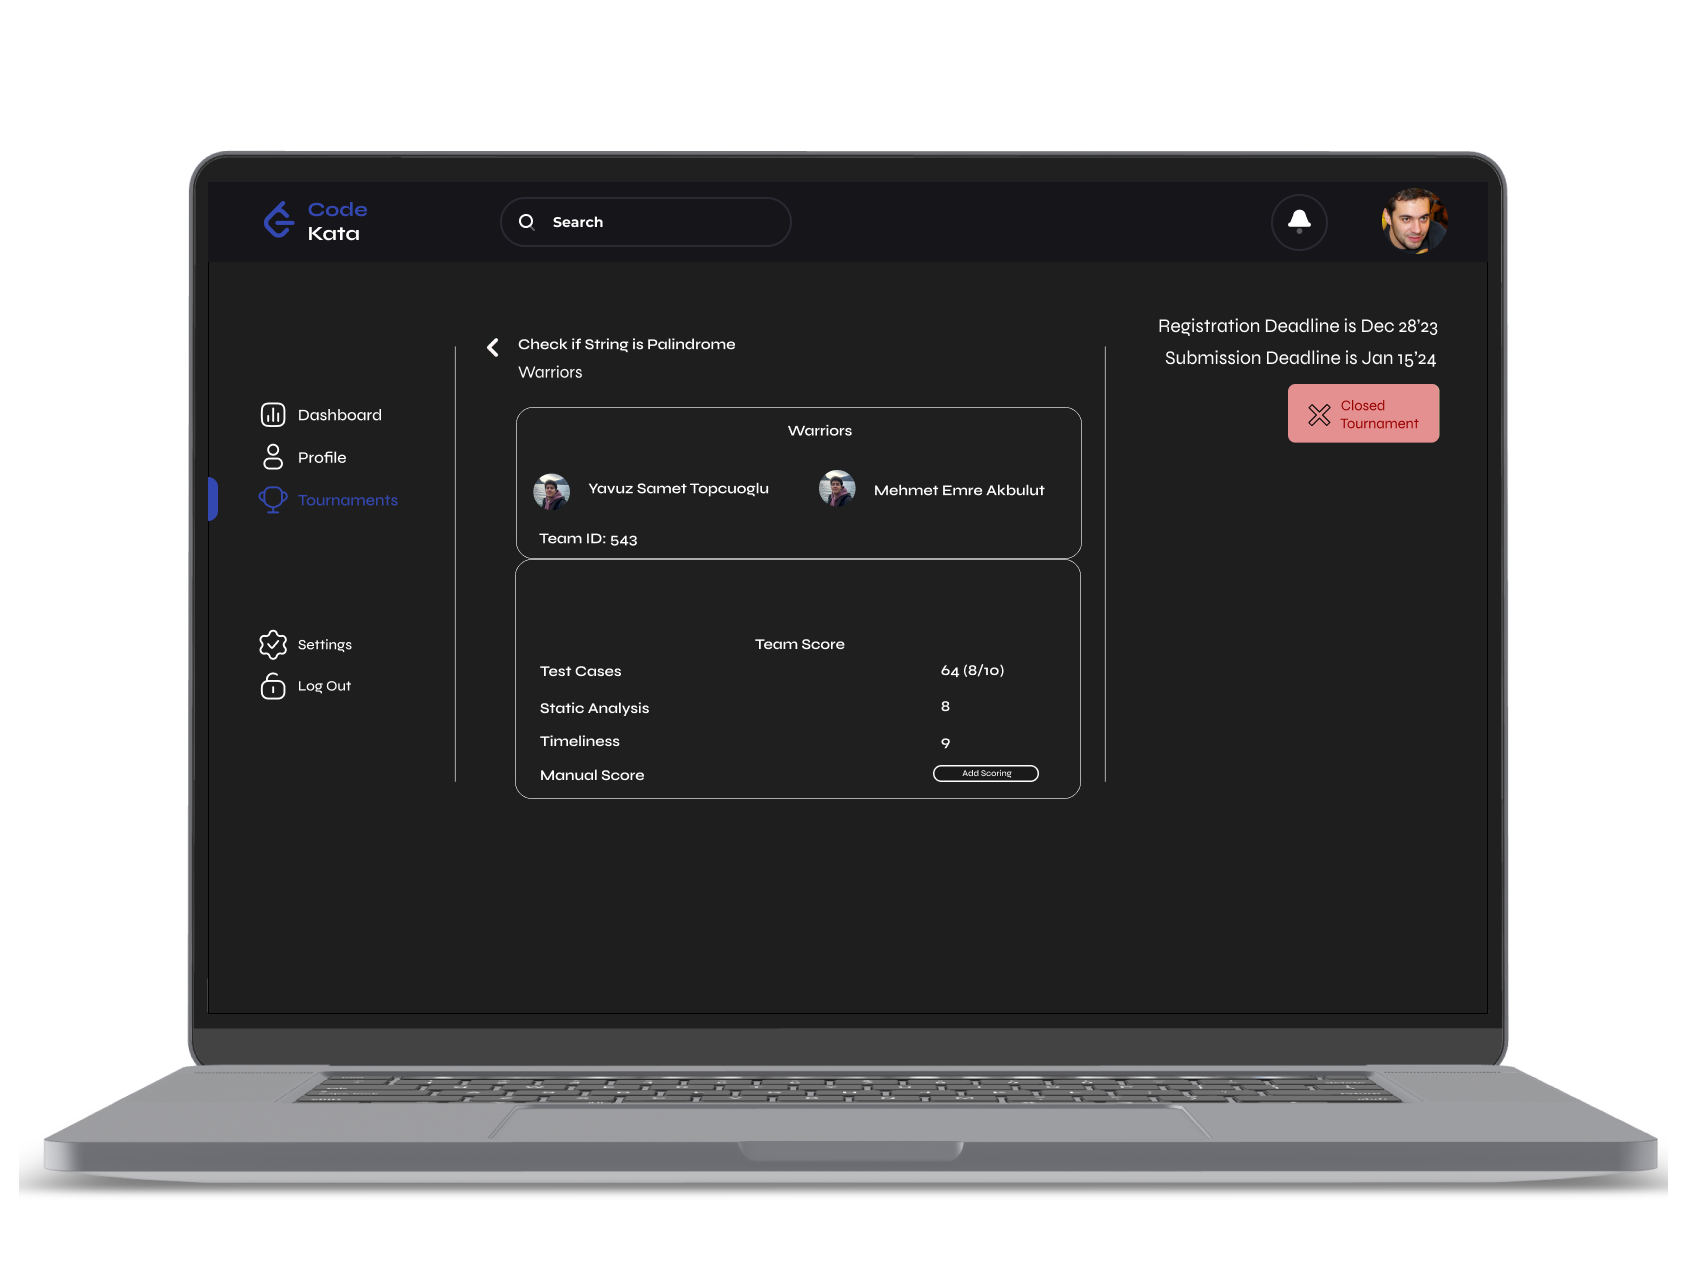
\includegraphics[scale=0.13]{Images/ui-ux/educator_team/educator_team_1.png}
% 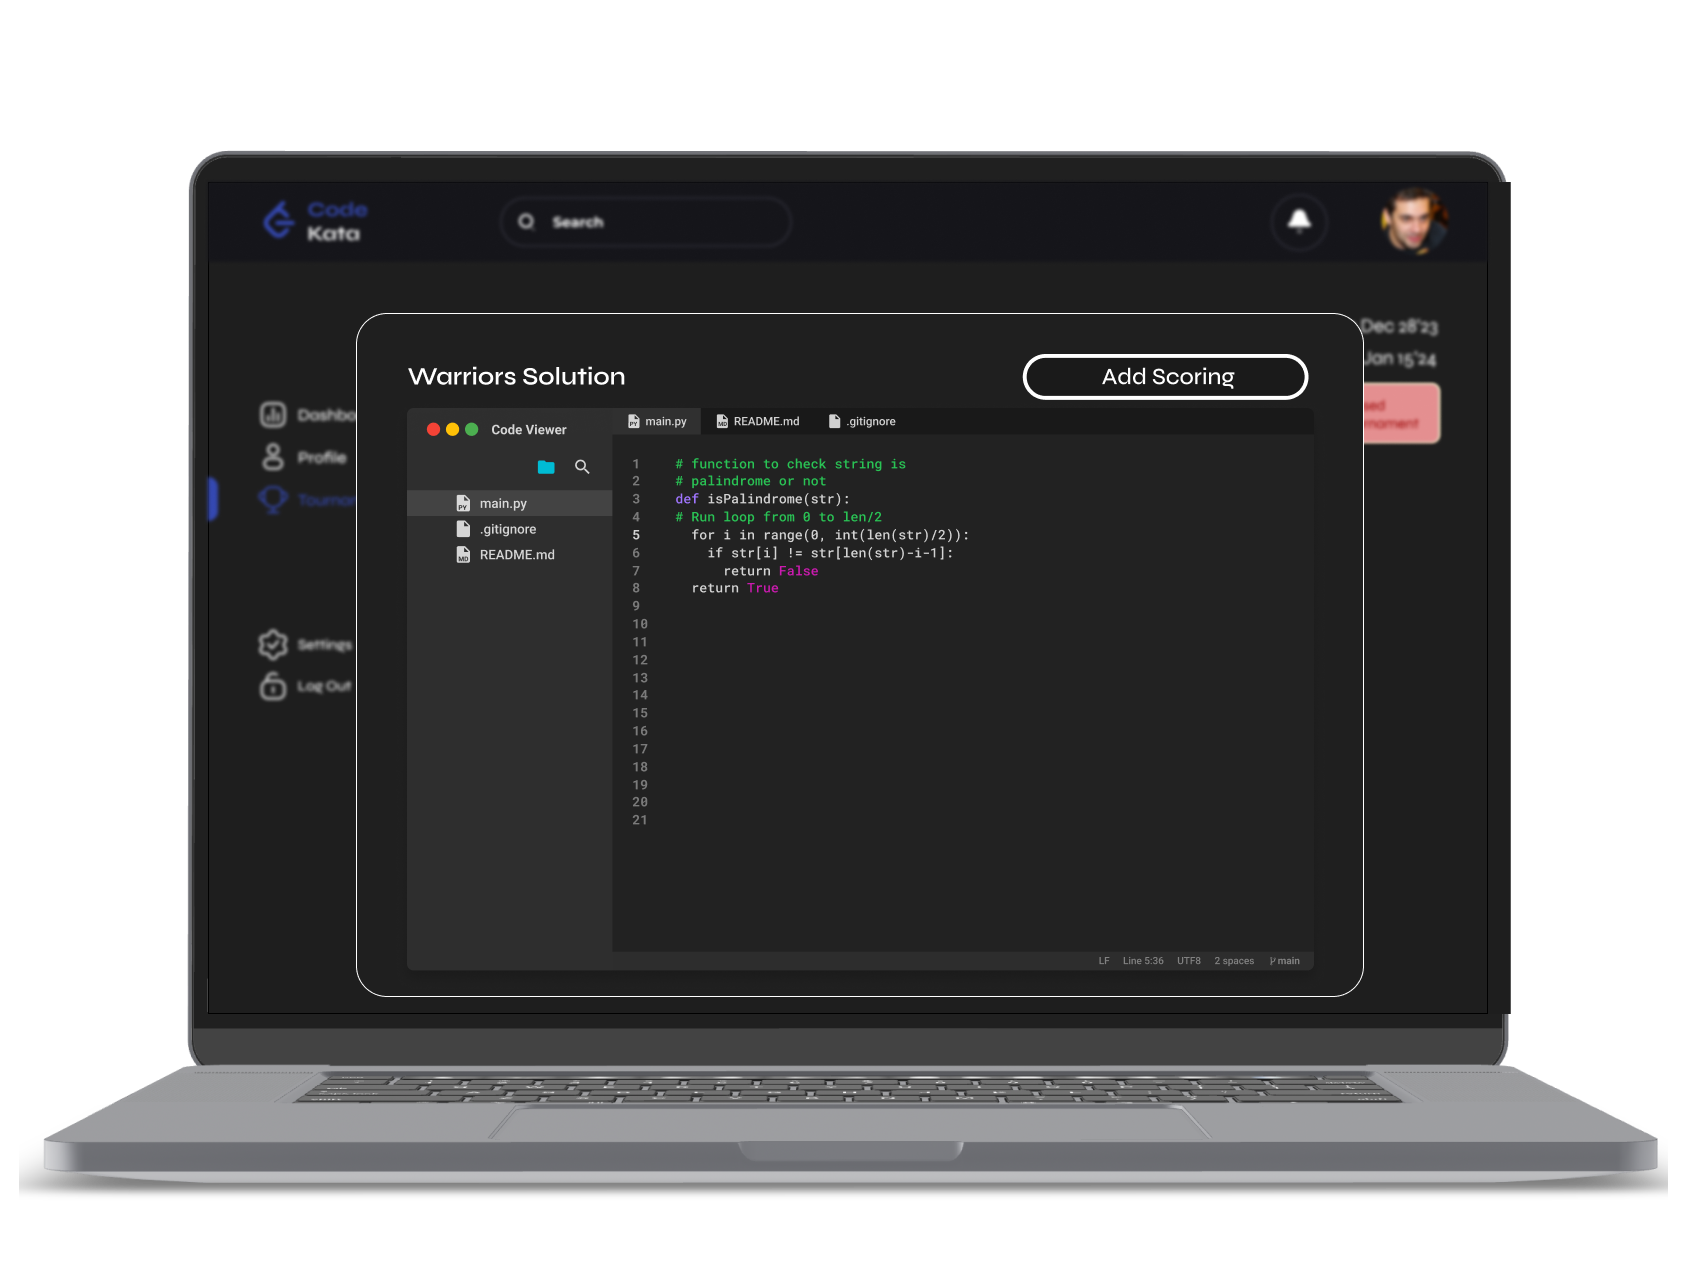
\includegraphics[scale=0.13]{Images/ui-ux/educator_team/educator_team_2.png}
% 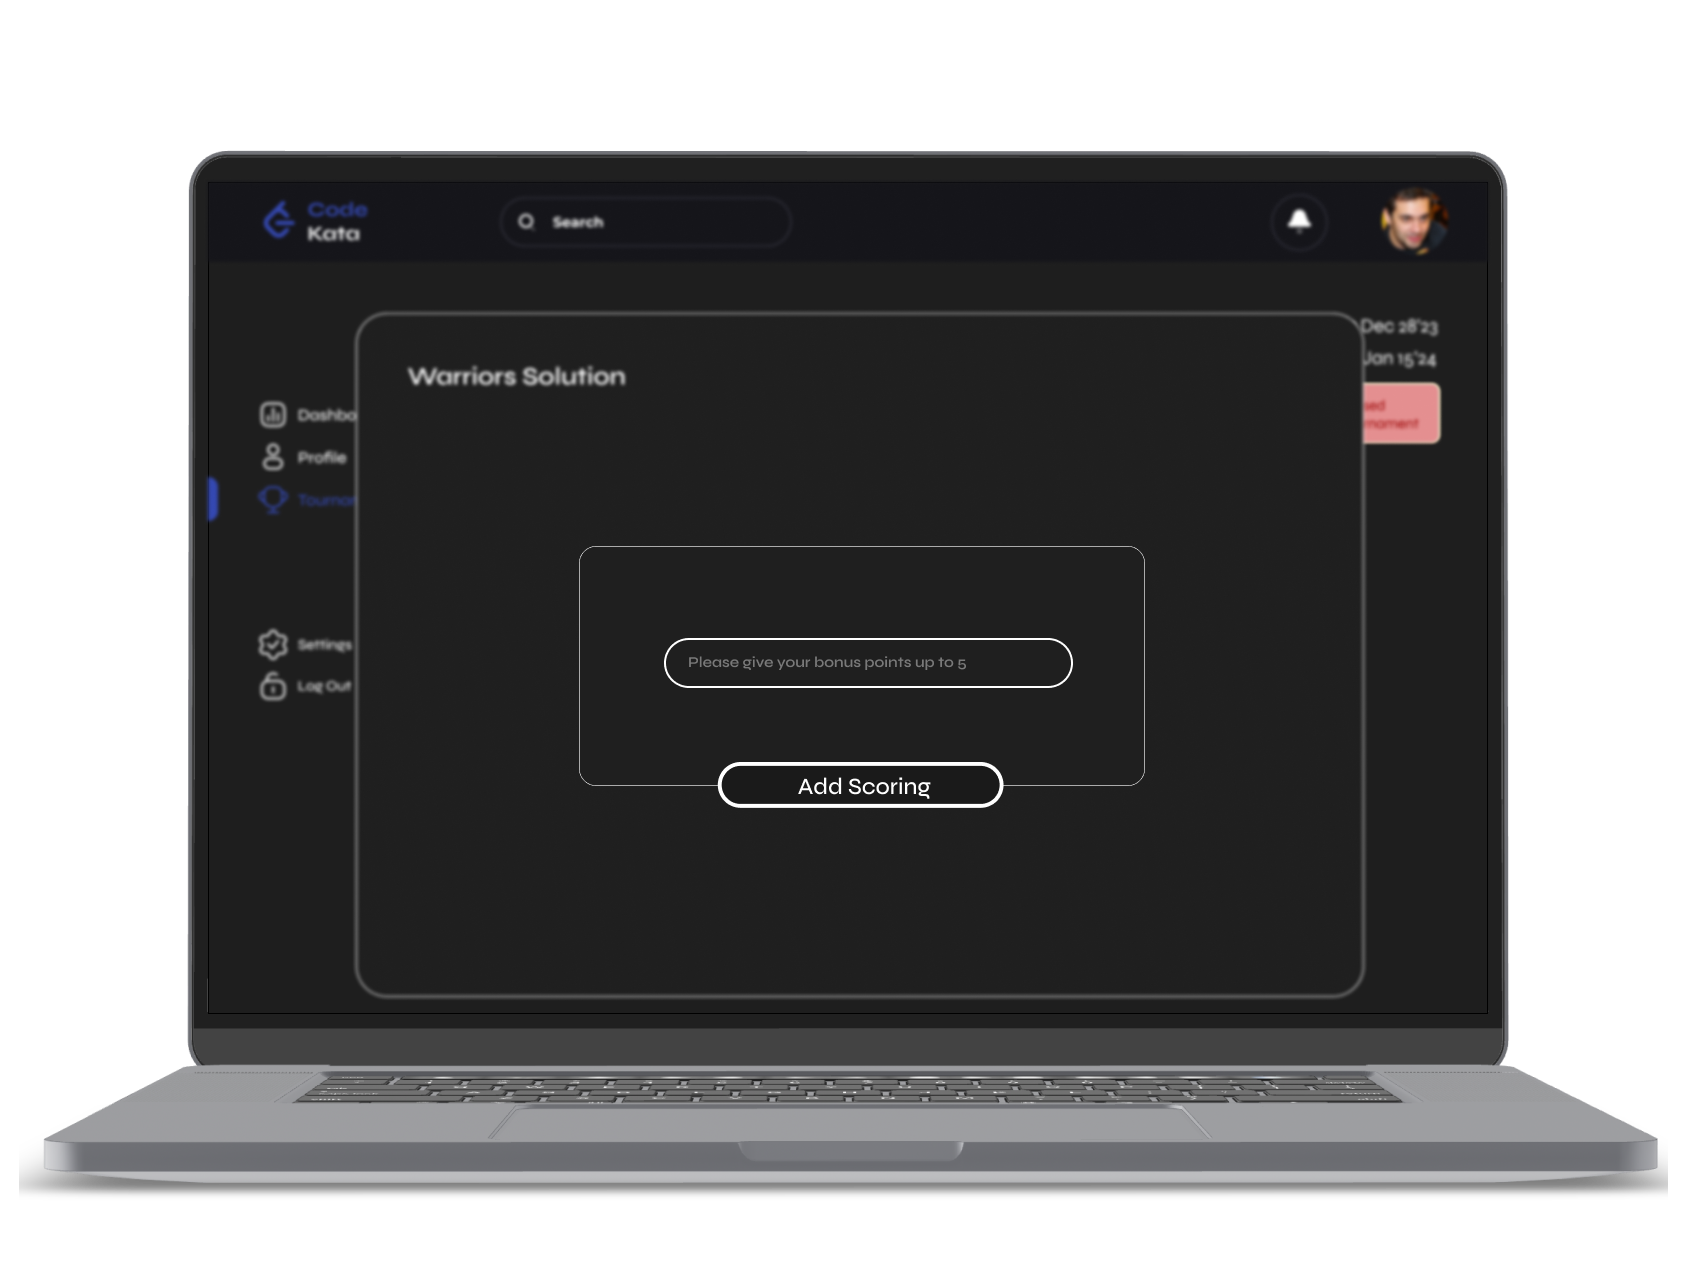
\includegraphics[scale=0.13]{Images/ui-ux/educator_team/educator_team_3.png}
% 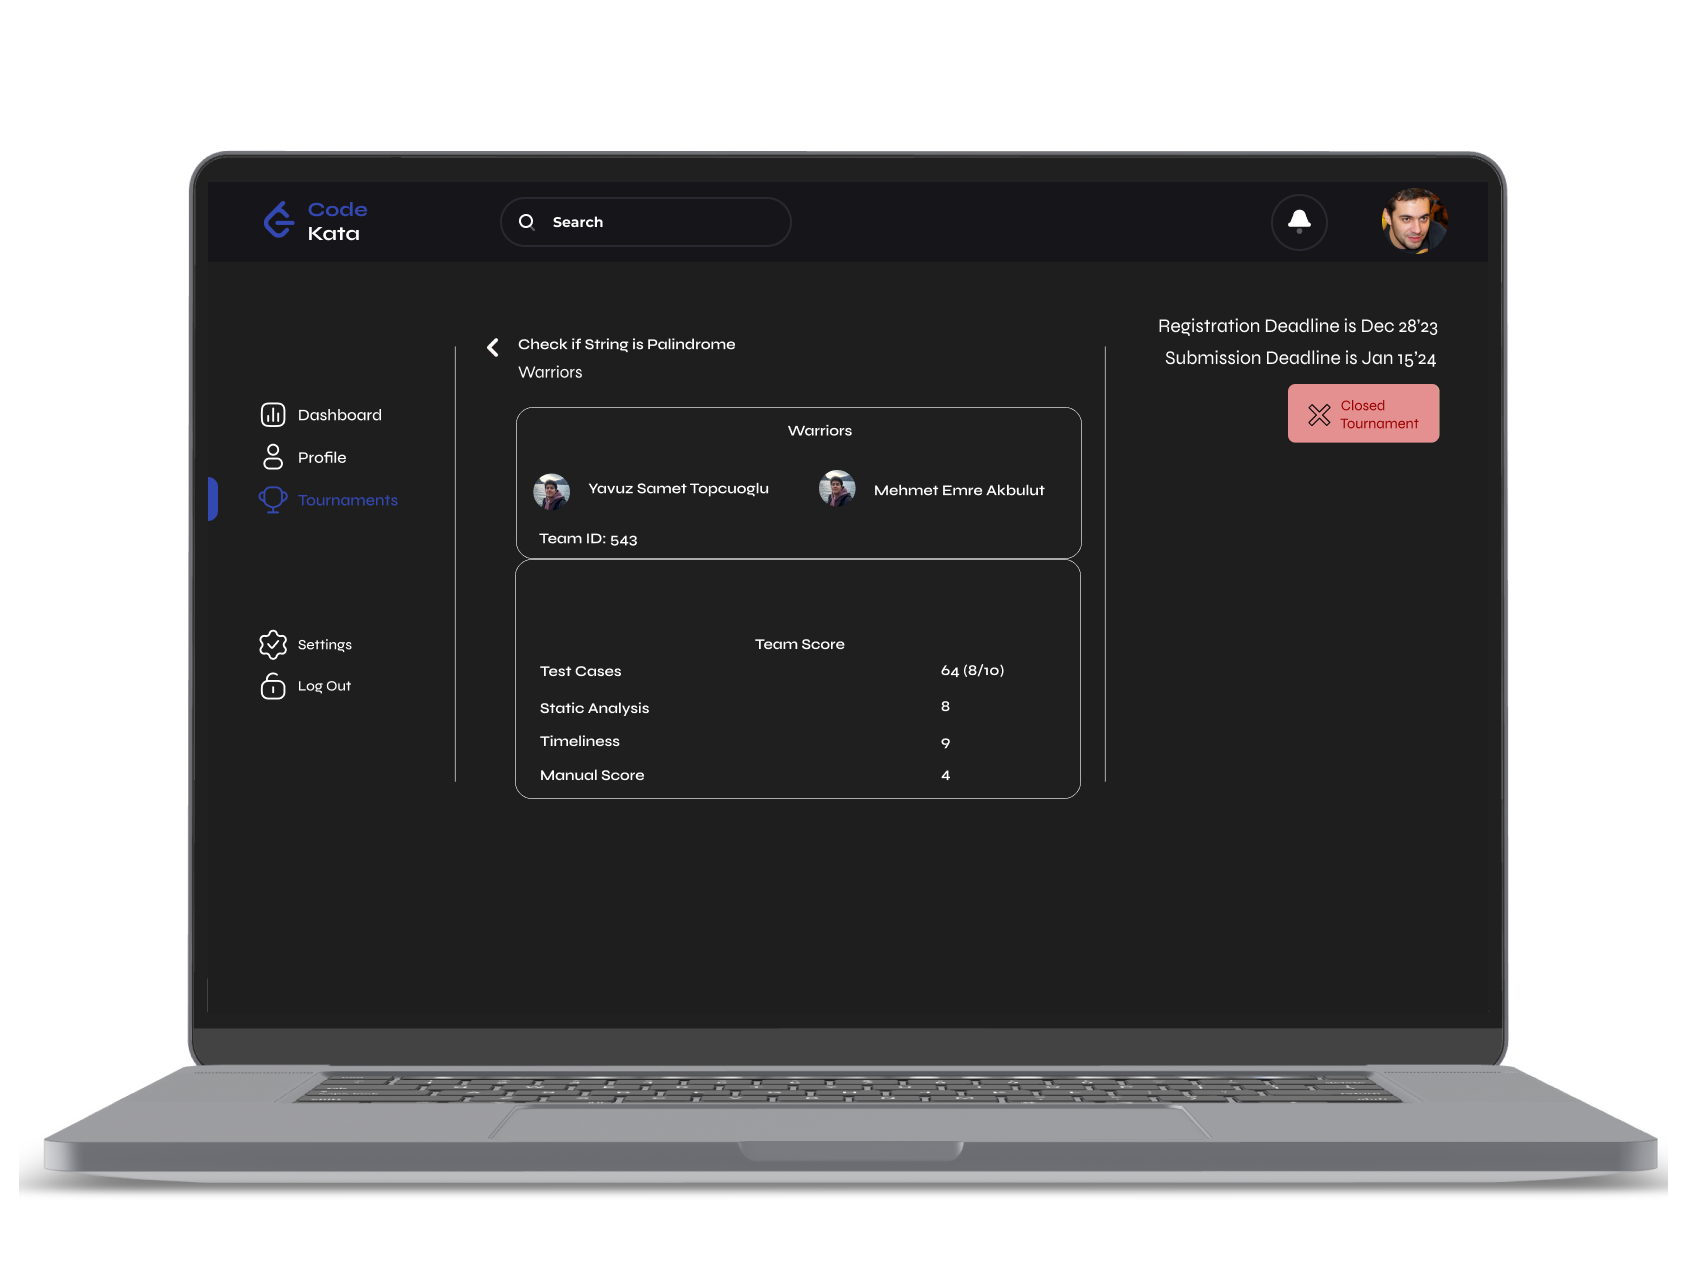
\includegraphics[scale=0.13]{Images/ui-ux/educator_team/educator_team_4.png}
%         (a) Educator, Team and Manual Scoring
% \end{center}
% \begin{center}
% 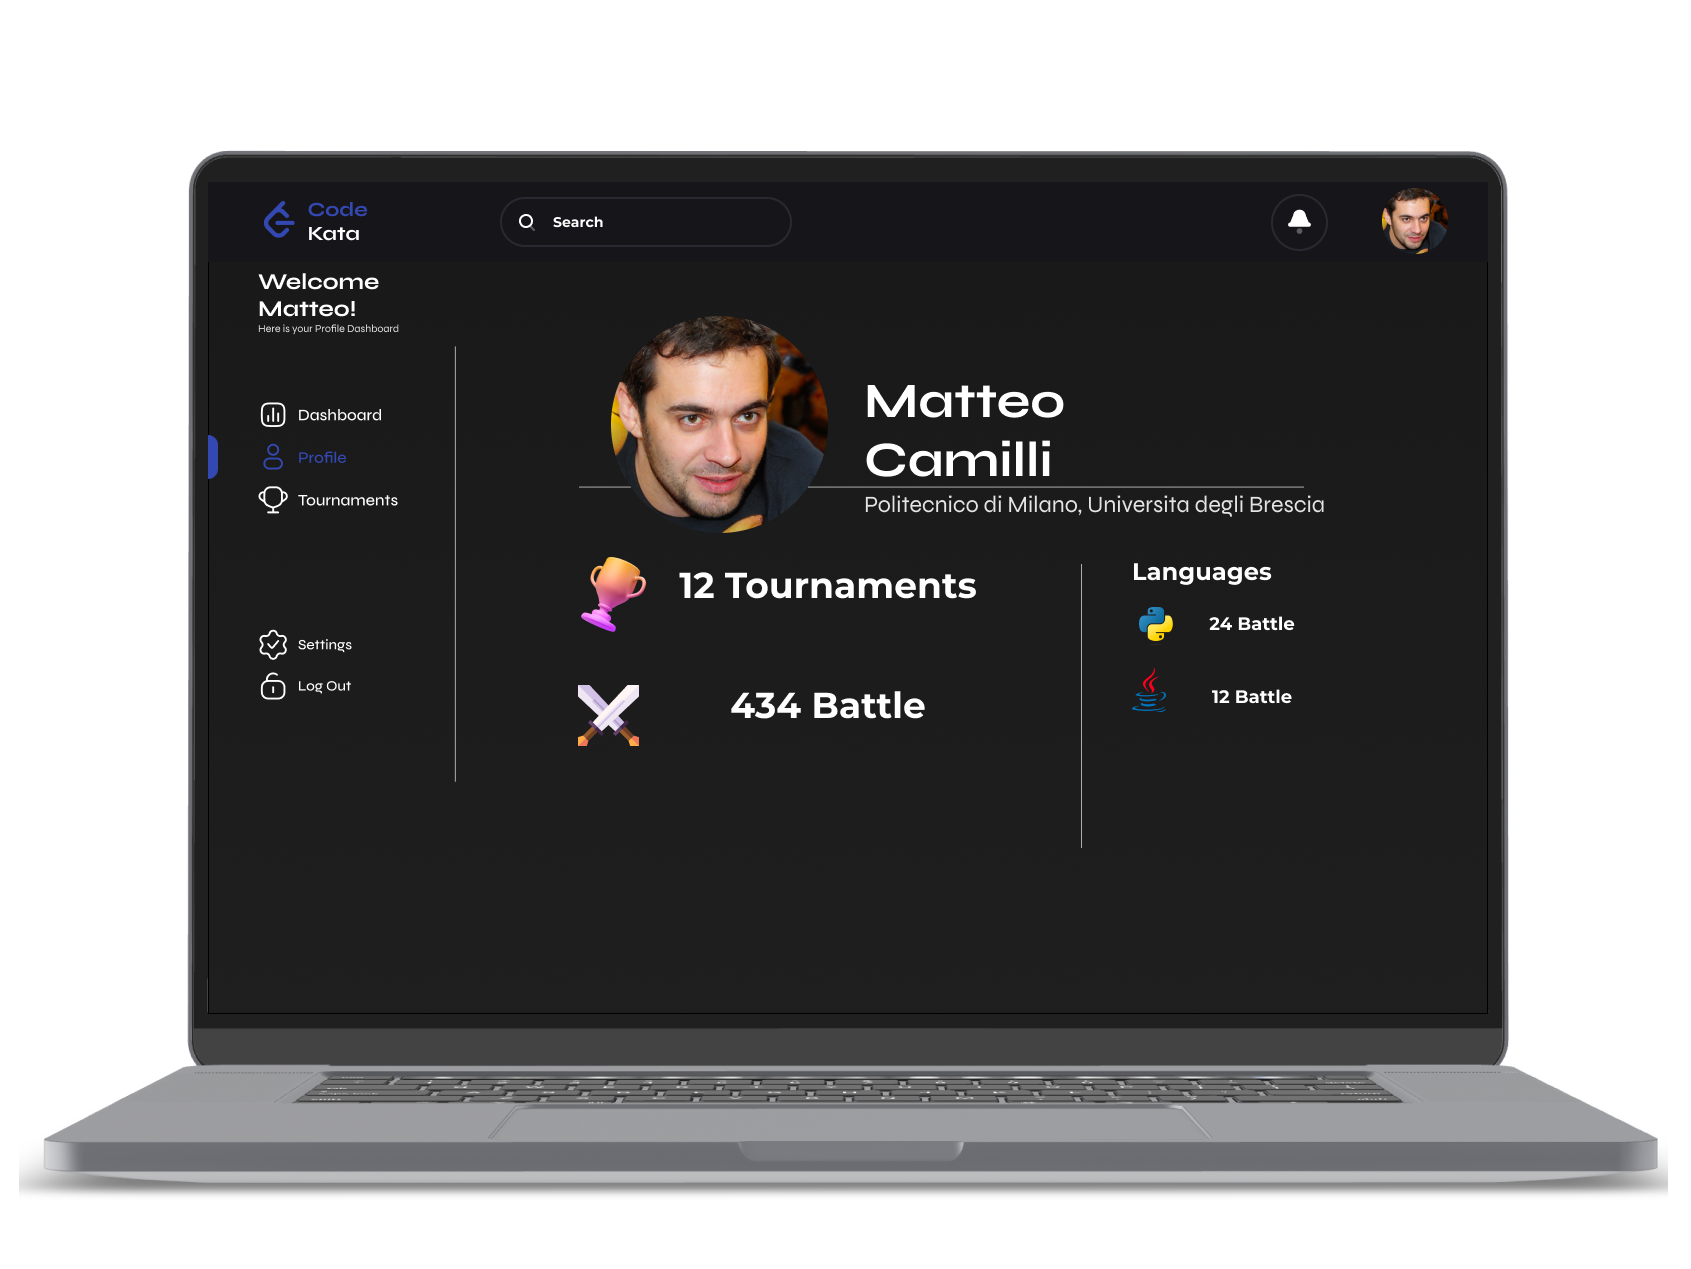
\includegraphics[scale=0.13]{Images/ui-ux/educator_profile_settings/educator_profile.png}
% 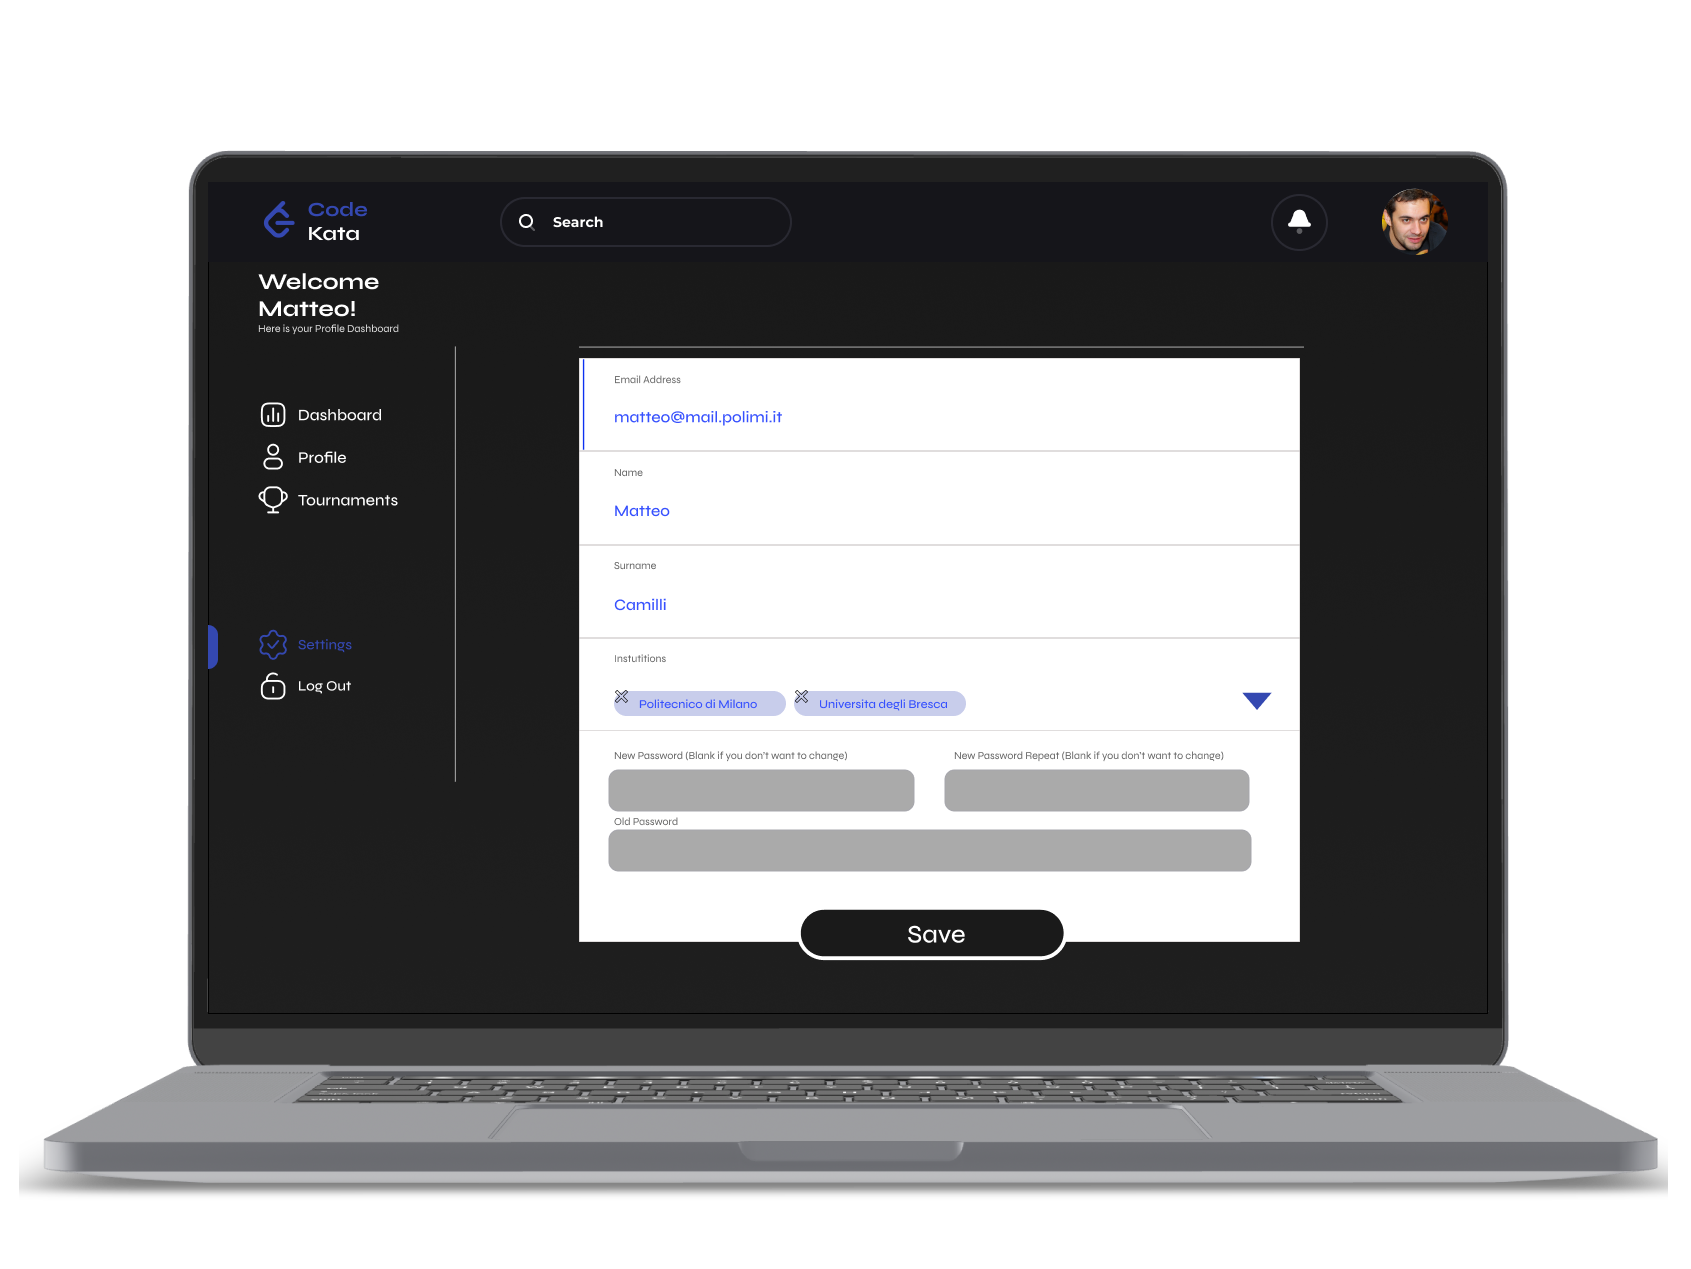
\includegraphics[scale=0.13]{Images/ui-ux/educator_profile_settings/educator_settings.png}
%         (a) Educator Profile and Settings
% \end{center}
\newpage
    
\subsubsection{Hardware Interfaces}
The CodeKataBattle platform operates entirely through web interfaces, eliminating the need for specialized hardware interfaces. Users can access the platform using standard web-enabled devices, such as computers, tablets, and smartphones. The platform is designed to function within a web browser, requiring no specific hardware beyond a device capable of running a modern browser and accessing the internet. This approach ensures broad accessibility without necessitating particular hardware configurations, making the platform versatile and user-friendly across various hardware setups. However, for optimal experience, at least 2GB of RAM and a minimum of 1GB of free space are recommended for browser caching and temporary files.

\subsubsection{Software Interfaces}
Our platform CKB interfaces with various software systems:

\begin{itemize}
    \item \textbf{Web Browsers:} Platform operates on web browsers. For universal access and easy use, it is compatible with major browsers like Chrome, Edge, Safari, Opera, and Firefox.

    \item \textbf{GitHub API:} Integrated for creating coding repositories and managing code \textit{submission} processes.

    \item \textbf{Sandboxing:} To create an isolated testing environment, our Sandbox Manager will utilise Docker.

    \item \textbf{Static Analysis Tool:} SonarQube API will be integrated for scoring the quality aspect of the code with static analysis. 

    \item \textbf{Database Technology:} Platform uses databases such as PostgreSQL.

    \item \textbf{Hosting:} Our platform uses Amazon Web Services EC2 for web server and database hosting.

    \item \textbf{Cloud File Storage:} The files will be stored using Amazon S3 services.

    \item \textbf{Email Service:} Amazon Simple Email Service SES will be used to send automated email notifications.
\end{itemize}

\subsubsection{Communication Interfaces}
Our platform utilises various communication systems:

\begin{itemize}
    \item \textbf{HTTPS:} For secure connection over the internet.

    \item \textbf{RESTful APIs:} We have RESTful APIs to communicate with the requests coming from GitHub Actions and the web application.

    \item \textbf{SMTP:} It is used to manage to send automated emails.
\end{itemize}

\subsection{Functional Requirements}
\subsubsection{Use Case Diagrams}
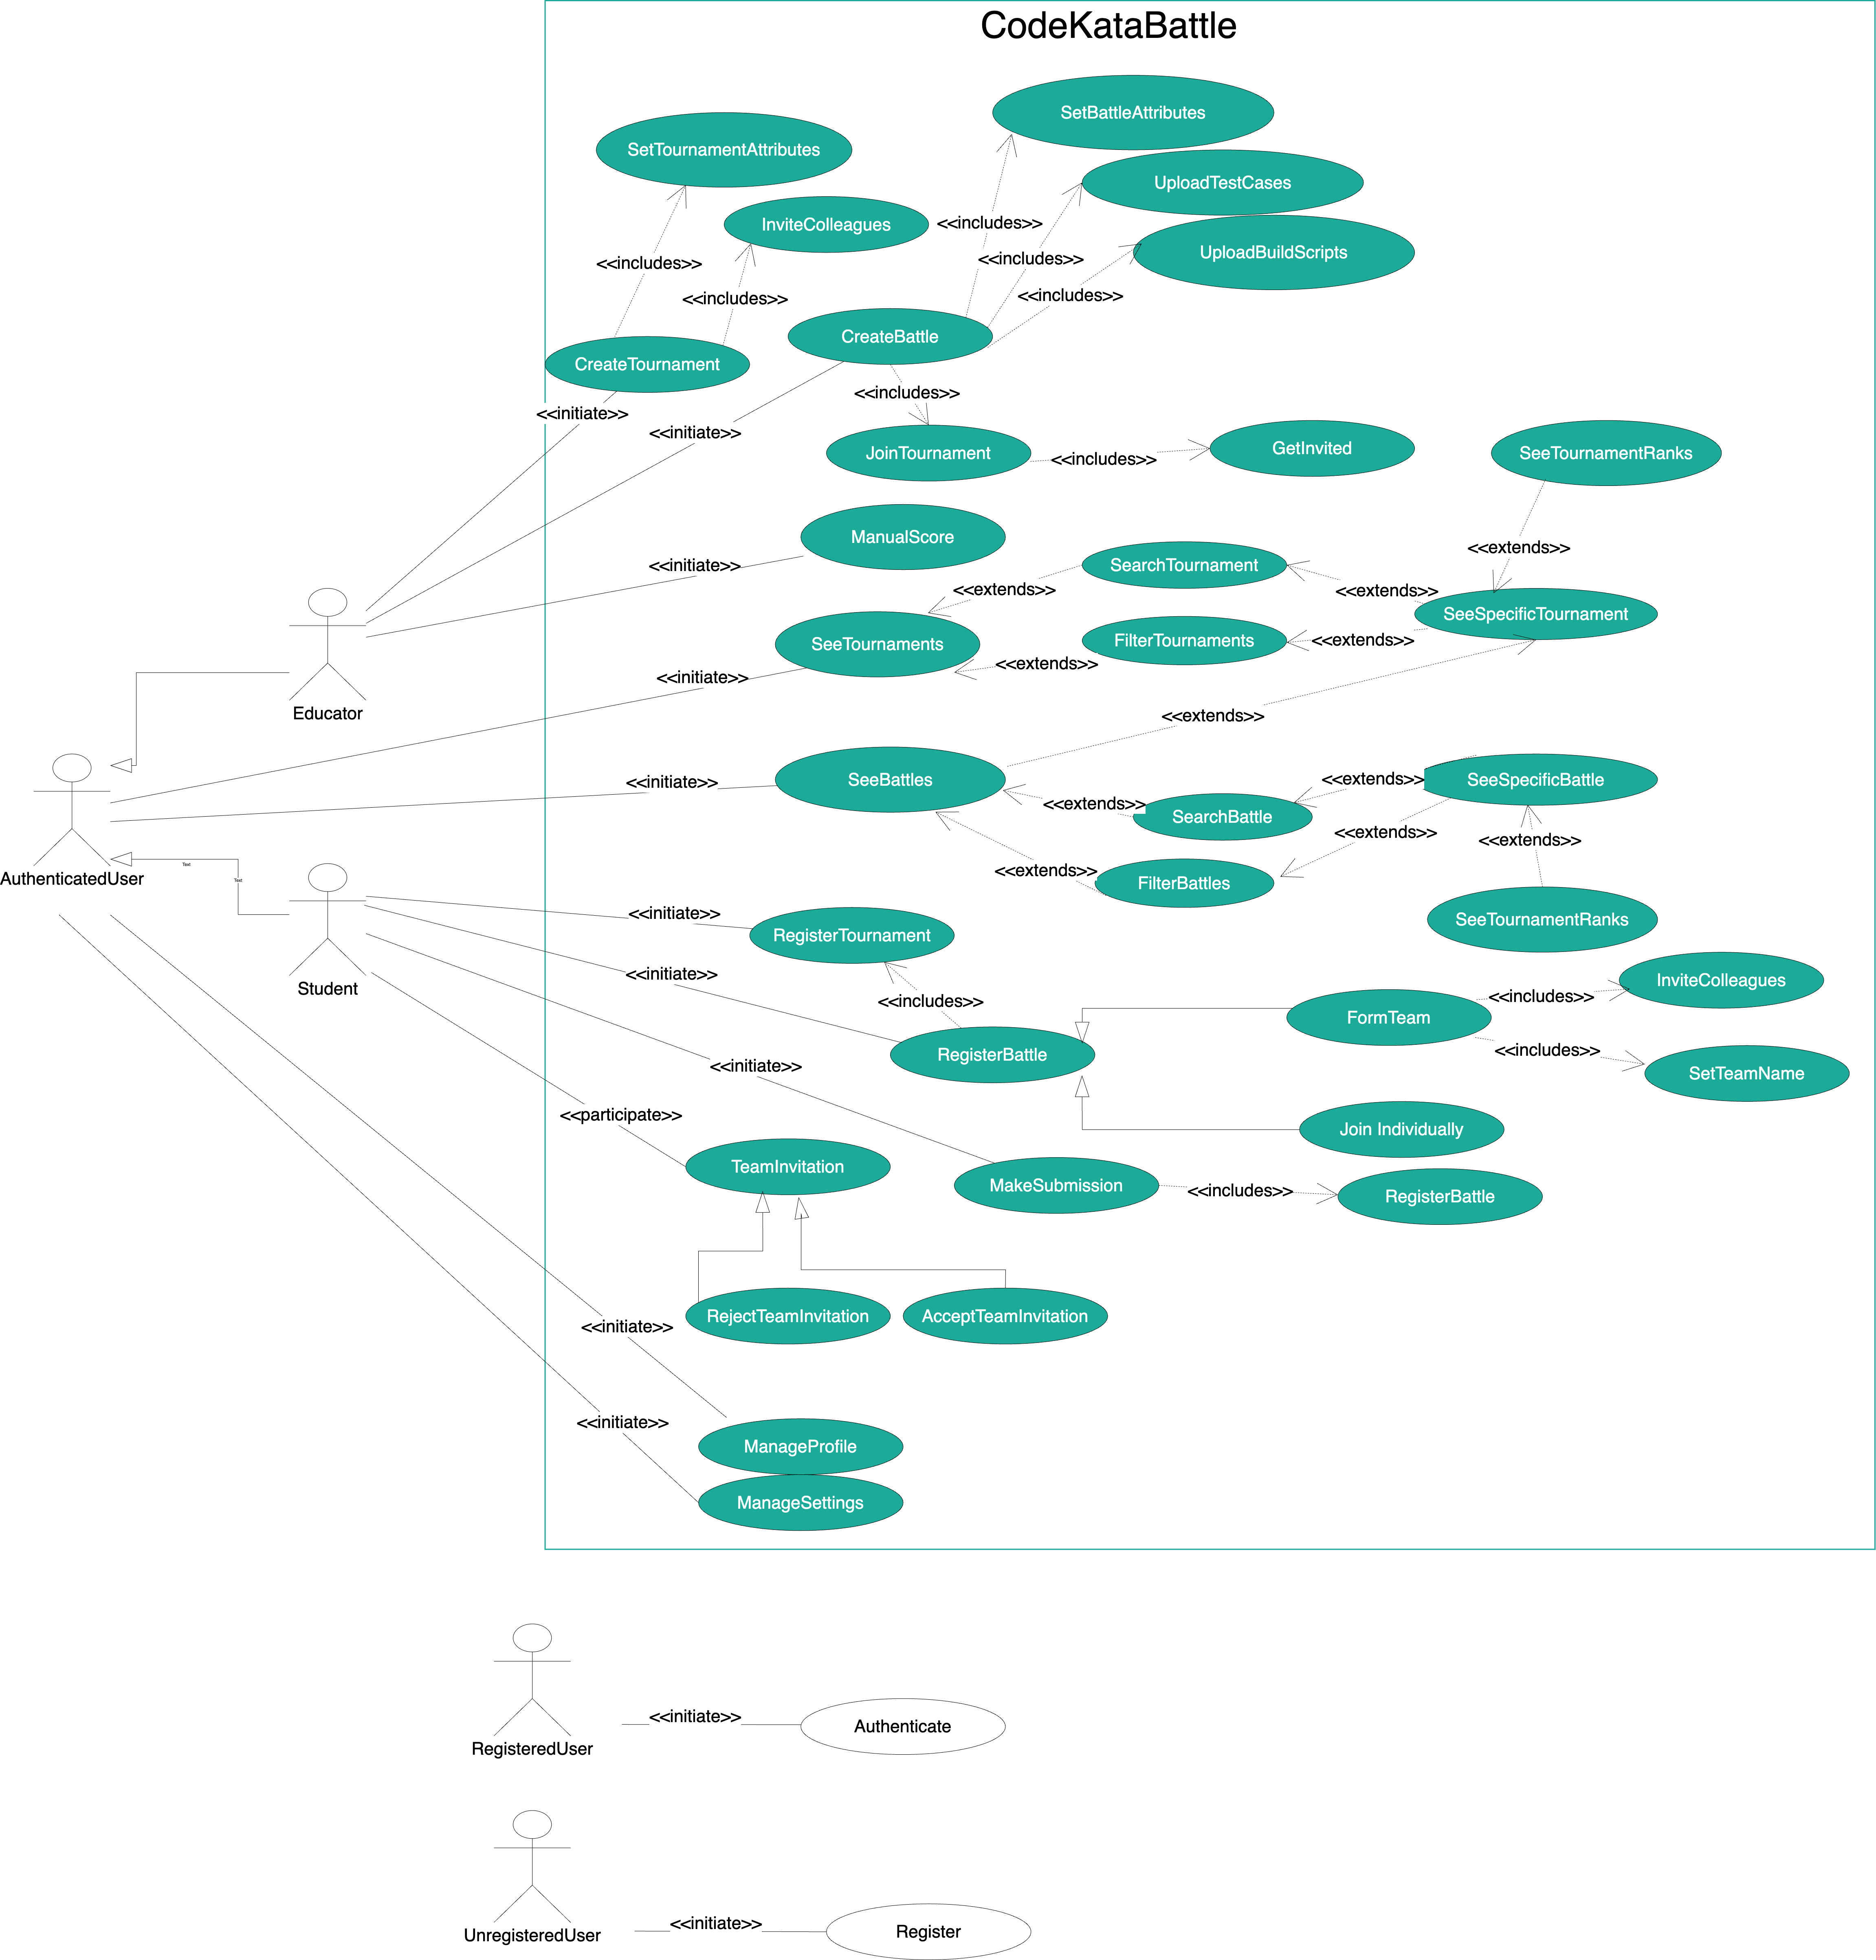
\includegraphics[scale=0.27]{Images/use_case_diagrams.drawio.png}
\newpage
\quad Unregistered User Actor has been used to illustrate the Registration Use Case. Similarly, the Registered User Actor has been used to show the Authentication Use Case. Other user actors are assumed to be registered and authenticated.

\quad Our system is composed of two main user types: Student and Educator. In the use case diagram, we showed common use cases with the Authenticated User actor. Authenticated User, simply every user registered to the platform, can view Tournaments, Battles, and their rankings with different filters and search options. Moreover, Registered User has the capability of viewing their profile and editing settings.

\quad Use case related Educator and Student Actors summarizes the goal of these users in the system.

\quad Invitee Student and Invitee Educator Actors are used to demonstrate use cases for tournament(for educators) and team(for students) invitations.

\quad GitHub System Boundary contains use cases about code submission with the participation of GitHub API Actor.





%------------------------------------------------------------------------------------------------------------------------------------------------
\clearpage
{\color{Blue}{\section{Formal Analysis Using Alloy}}}
\label{sect:alloy}
In the formal analysis of the Alloy model for "CodeKataBattle," our primary aim is to establish a robust and meaningful representation of a coding tournament environment. This model intricately captures various elements such as tournament, battle, educators, students and relations among them.

\\
At the heart of the model there are signatures representing Tournament, Battle, Educator, Student, Team and Battle Score. The model also defines relationships and constraints, ensuring logical coherence and real-world applicability. For instance, it enforces unique emails for each user and stipulates that every user is either an educator or a student. This Alloy model ensures that Battle and Tournament constraints are fulfilled. Also model  highlights some of the constraints related to Educators and Students.  Main objective is the defining and checking some constraints related to these signatures, creating a world with requirements and implementing some assertions with respect to goals.
\\
In this model, UML Diagrams, Domain Assumptions and Requirements are used to support the model. Because of this, Alloy Signatures are not the exact version of Class Diagram. It is more detailed and defined to include aspects of the software product to be created according to certain Domain assumptions, Requirements and Goals. 

\\
A notable feature of this model is its ability to simulate the dynamic process of coding tournaments and battles. It captures the lifecycle of a tournament from creation to conclusion, including the creation of battles, team formations, code submissions, and scoring mechanisms. The model's flexibility allows for various scenarios, such as battles with manual scoring enabled and diverse programming language requirements.
\\
By running this model in Alloy, we can generate specific "worlds" that demonstrate its soundness and correctness. These worlds represent possible states of the system under different conditions, providing concrete examples of how the model functions in practice. 
\\
This model demonstrates that our method of building the system is both logical and coherent. Essentially, the connections between classes and the applied constraints yield an outcome that is both practical and beneficial. Such a result also validates the rationale behind the modeling process.

\\
In summary, the Alloy model is a comprehensive and flexible tool for simulating and analyzing coding tournaments and battles. Its ability to model complex interactions and enforce constraints makes it a valuable resource for understanding and improving software product.


    
    \begin{lstlisting}[language=alloy]
module CodeKataBattle


//These can be Enum also 
abstract sig Language {}
one sig PYTHON extends Language {}  
one sig JAVA extends Language {}
one sig C extends Language {}
one sig CPP extends Language {}
one sig JAVASCRIPT extends Language {}
one sig RUBY extends Language {}
one sig GO extends Language {}
one sig RUST extends Language {}
one sig CSHARP extends Language {}
abstract sig QualityAspect {}
one sig COMPLEXITY, DUPLICATIONS, MAINTAINABILITY, RELIABILITY, SECURITY, CLEAN_CODE extends QualityAspect {}

//These can be Enum also
abstract sig  TournamentStatus {}
one sig REG_OPEN, ONGOING, CLOSED extends TournamentStatus{}
//These can be Enum also
abstract sig BattleStatus {}
one sig REG_OPEN_BATTLE, ONGOING_BATTLE, CONSOLIDATION, CLOSED_BATTLE extends BattleStatus{}

// Basic types
abstract sig Bool {}
one sig TRUE extends Bool {} 
one sig FALSE extends Bool {}

sig Time{
time: one Int
} {time>0}

//These fields are removed from User for the sake of simplicity because they are not related to anything but user specific attributes.  They can be unique or same, no check in the system related to this.
//sig Password{}
//sig Name{}
//sig Surname{}


//Signatures related to statuses of tournaments and battles
abstract sig Notification{}
sig TournamentCreated extends Notification{
  tournamentCreated: one Tournament
}
sig TournamentEnded extends Notification{
tournamentEnded: one Tournament
}
sig TournamentInvited extends Notification{
tournamentInvited: one Tournament
}
sig BattleStarted extends Notification{
battleStarted: one Battle
}
sig BattleFinished extends Notification{
battleFinished: one Battle
}

//Fundamental Signatures
sig Institution{}
sig TournamentTitle{}
sig TournamentDescription{}

sig TeamName{}

sig URL{}

sig Email{}
sig User {
    email: one Email,
    notifications: set Notification
}

sig Educator extends User {
    var creates: set Tournament,
    var contributesTo: set Tournament,
    var createsBattle: set Battle,
    institutions: set Institution,
    var givenManualScores: set ManualScore
}

sig Student extends User {
    var registers: set Tournament,
    var tournamentScores: Tournament -> lone Int,
    institution: lone Institution,
}

sig Tournament {
    title: one TournamentTitle,
    description: one TournamentDescription,
    registrationDeadline: one Time,
    closingTime: lone Time,
    var status: one TournamentStatus,
    var hasBattle: set Battle,
    var subscribers: set Student,
} {
     registrationDeadline.time < closingTime.time

}

//In Alloy range of integers is very low, so values of integers are not the real values, just mock
sig ScoringWeights{
    TEST_CASES:  Int,
    TIMELINESS:  Int,
    QUALITY:  Int
    } {
     TEST_CASES > 0 && TIMELINESS > 0 && QUALITY>0 && plus[plus[TEST_CASES,TIMELINESS],QUALITY]=6
    }
	
sig Team {
    teamName: one TeamName,
    hasMember: some Student,
    submits: lone Submission,
}

sig BattleTitle {}
sig Battle {
    title: one BattleTitle,
    codeKata: one CodeKata,
    minStudentsPerGroup: one Int,
    maxStudentsPerGroup: one Int,
    creationTime: one Time,
    registrationDeadline: one Time,
    submissionDeadline: one Time,
    var status: BattleStatus,
    allowedLanguages: some Language,
    chosenQualityAspects: some QualityAspect,
    var teams: set Team,
    scoringWeights: one ScoringWeights,
    manualScoringEnabled: one Bool,
    battleRepositoryUrl: lone URL,
    sandboxEnvironment: SandboxEnvironment,
} {
  registrationDeadline.time < submissionDeadline.time &&
  minStudentsPerGroup<=maxStudentsPerGroup &&
  minStudentsPerGroup>=0 &&
  maxStudentsPerGroup>=0 
 }

sig Code{}
sig Submission{
code: one Code,
repositoryUrl: one URL,
commitTime: one Time,
score: one BattleScore,
sandboxEnvironment: SandboxEnvironment
}
sig ManualScore{
    score: one Int
} {score>=0}
sig BattleScore {
    testCasesScore: one Int,
    timelinessScore: one Int,
    qualityScore: one Int,
    manualScore: lone ManualScore,
    totalScore: one Int
} {
   totalScore = calculateBattleScore[this]
   testCasesScore >=0
   timelinessScore >=0
   qualityScore >= 0
}

fun calculateBattleScore(bs:BattleScore): Int {
    bs.testCasesScore + bs.timelinessScore + bs.qualityScore
}

sig BattleDescription{}
sig CodeKata {
    description: one BattleDescription,
    testCases: some TestCase,
    buildScripts: some BuildScript
} 

sig TestCase {
language: one Language
}

sig BuildScript {
language: one Language
}


//Each  battle has a sandbox environment that runs the code
sig SandboxEnvironment{}

// Relationships and constraints


//Every user has unique email 
fact EmailsAreUnique{
no disjoint u1, u2: User | u1.email = u2.email
}

//Every user is eiher Educator or Student
fact AllUsersAreEitherEducatorOrStudent {
    all u: User |
        (u in Educator and u not in Student) or (u in Student and u not in Educator)
}

// Each team must be associated with a battle and have members within the specified group size constraints.
fact TeamsWithinGroupSizeConstraints {
    all t: Team |some b: Battle	|	t in b.teams	and	#t.hasMember >= b.minStudentsPerGroup and #t.hasMember <= b.maxStudentsPerGroup
}

//In a battle there must be test cases and build scripts for each allowed language
fact ArtifactsProvided {
    all b: Battle | {
        all l: b.allowedLanguages | {
            one tc: TestCase | tc.language=l	and	tc in b.codeKata.testCases
            one bs: BuildScript| bs.language=l and bs in b.codeKata.buildScripts
        } 
    }
}

//no other than allowed languages
fact TestCasesAndBuildScriptsForAllowedLanguagesOnly {
    all b: Battle | 
            b.codeKata.testCases.language in b.allowedLanguages and b.codeKata.buildScripts.language in b.allowedLanguages
}



// Each Test Case and Build Script Belongs To One Code Kata
fact ArtifactsBelongsToOneCodeKata {
    // For every TestCase, there is exactly one CodeKata that it's related to
    all tc: TestCase | one ck: CodeKata | tc in ck.testCases
    
    // For every BuildScript, there is exactly one CodeKata that it's related to
    all bs: BuildScript | one ck: CodeKata | bs in ck.buildScripts
}

// Every tournament is created by exactly one educator
fact UniqueEducatorForTournament {
    all t: Tournament | one e: Educator | e.creates = t
}

fact UniqueBattleForCodeKata {
    // Every CodeKata is associated with exactly one Battle
    all ck: CodeKata | one b: Battle | ck = b.codeKata
}


// Every tournament is contributed to by at least one educator which is the creator of the tournament
fact CreatorContributesTournament {
    all t: Tournament | one e: Educator | t = e.creates and t in e.contributesTo
}

// Every battle is created by exactly one educator
fact UniqueCreatorForBattle {
    all b: Battle | one e: Educator | e.createsBattle = b
}

// Every battle is associated with exactly one tournament
fact UniqueTournamentForBattle {
    all b: Battle | one t: Tournament | b in t.hasBattle and 
        all tOther: Tournament - t | b not in tOther.hasBattle
}

//for consitency
fact SubscribersAreRegistered {
    all t: Tournament, s: Student |  t in s.registers implies s in t.subscribers 
}



// Every educator can create battles only for tournaments they contribute to
fact ContributerCreatesBattle{
    all e: Educator, b: Battle | b in e.createsBattle implies b in e.contributesTo.hasBattle
}

// Unique battle titles within a tournament
fact UniqueBattleTitle{
    all t: Tournament | no disjoint b1, b2: t.hasBattle | b1.title = b2.title
}

// Unique tournament titles
fact UniqueTournamentTitles {
    no disjoint t1, t2: Tournament | t1.title = t2.title
}

// Unique team names within a battle
fact UniqueTeamNamesWithinBattle {
    all b: Battle | no disjoint t1, t2: b.teams | t1.teamName = t2.teamName
   all tn:TeamName	|	one t: Team	|	t.teamName=tn
}

// Ensure submission constraints
fact EveryManualScoreHasAScoreAndSubmission {
    all ms: ManualScore | 
        one bs: BattleScore | bs.manualScore = ms
}

fact EveryManualScoreHasAScoreAndSubmission {
    all bs: BattleScore | 
        one s: Submission | bs in s.score
}

fact EveryManualScoreHasAScoreAndSubmission {
    all s: Submission | 
        one t: Team | s in t.submits
}

fact EveryManualScoreHasAScoreAndSubmission {
    all t: Team | 
        one b: Battle | t in b.teams
}


fact EveryCodeHasASubmission {
    // For every Code, there exists a Submission that has this score
    all cd: Code | one s: Submission | s.code = cd
}

// A student's submission must be their own work and associated with a team that is part of a battle. A domain assumption
fact UniqueSubmissionRepositoryUrlWithinBattle {
    all url: URL | one s: Submission | s.repositoryUrl = url
}

// A student can only be part of at most one team per battle
fact StudentInAtMostOneTeamPerBattle {
    all b: Battle | no disj t1, t2: b.teams | some s: Student | s in t1.hasMember and s in t2.hasMember
}


// Students can only be part of teams for battles in tournaments they have registered for.
fact StudentTeamRegistrations {
    all s: Student | all t: s.registers | let battles = t.hasBattle |
    all team: Team | s in team.hasMember implies team in battles.teams
}


// There is no created battle if tournament status is REG_OPEN
fact noBattlesInRegistration {
    all t: Tournament | t.status = REG_OPEN implies no t.hasBattle
}

// There is no submission  if battle status is REG_OPEN_BATTLE
fact noSubmissionsAndRepoForOpenBattles {
    all b: Battle | b.status = REG_OPEN_BATTLE implies {
        no t: b.teams | some t.submits and
        no b.battleRepositoryUrl
    }
}


fact AllBattlesClosedIfTournamentClosed {
    all t: Tournament | t.status = CLOSED implies all b: t.hasBattle | b.status = CLOSED_BATTLE
}


// Battle registration time is less than Tournament closing Time. It is check for closed tournaments. A closed tournament can not have a battle with creation time later than closing time
fact BattlesWithinTournamentClosingTime {
    all t: Tournament, b: t.hasBattle | one t.closingTime && b.creationTime.time < t.closingTime.time
}

fact ManualScoreConstraint {
    all bs: BattleScore |
       one  bs.manualScore  implies bs.manualScore.score >= 0 && bs.manualScore.score <= 2
}


//Scores should be in range 0 and their weights
fact ScoreWithinWeightRange {
    all t: Team | some t.submits implies {
        let s = t.submits.score |
            // Find the battle that includes this team
            some b: Battle | t in b.teams and {
                let weights = b.scoringWeights |
                s.testCasesScore >= 0 and s.testCasesScore <= weights.TEST_CASES and
                s.timelinessScore >= 0 and s.timelinessScore <= weights.TIMELINESS and
                s.qualityScore >= 0 and s.qualityScore <= weights.QUALITY
            }
    }
}

fact enforceManualScoringRules {
    all b: Battle | {
        // If the battle is in consolidation and manual scoring is enabled,
        // there must be a manual score for each battle score
        (b.status = CLOSED_BATTLE and b.manualScoringEnabled = TRUE) implies {
            all s: b.teams.submits.score | some ms: ManualScore | ms in s.manualScore
        }
        
        // If manual scoring is not enabled, the status cannot be CONSOLIDATION
        (b.manualScoringEnabled = FALSE) implies b.status != CONSOLIDATION
        
        // If the battle is in before consolidation or manual scoring is not enabled,
        // there cannot be a manual score for any battle score
        (b.status = REG_OPEN_BATTLE  or b.status = ONGOING_BATTLE or b.manualScoringEnabled = FALSE) implies {
            all s: b.teams.submits.score | no s.manualScore
        }
    }
}


//This fact enforces the rule that if a ManualScore exists for a BattleScore in a Battle, 
//it must have been given by the Educator who created that Battle. 
//If there is no ManualScore, this fact does not impose any additional requirements.
// In other words, it only applies when a ManualScore is present.
fact manualScoresGivenByCreator {
    all b: Battle, s: b.teams.submits.score, ms: s.manualScore | {
        some e: Educator | e.createsBattle = b and ms in e.givenManualScores
    }
}

//if a tournament is created (exists), it should be in Student's notification with as TournamentCreated notification, for every tournament exist there must be a notification about it in their notifications field.
fact notificationForTournamentCreation {
    all t: Tournament, s: Student | 
        one n: s.notifications | n in TournamentCreated and n.tournamentCreated = t
}

//if tournament is ended (status is CLOSED), it should be in Student's notification with as TournamentEnded notification, for every tournament ended there must be a notification about it in their notifications field.
fact notificationForTournamentEnding {
    all t: Tournament | t.status = CLOSED implies 
        all s: Student | s in t.subscribers implies 
            one n: s.notifications | n in TournamentEnded and n.tournamentEnded = t
}

fact TournamentEndedNotificationMeansTournamentEnded {
    all n: TournamentEnded | n.tournamentEnded.status = CLOSED
}


// if an educator is contributes to a tournament but not a creator, there must be a notification in its notifications with a TournamentInvited notification. 
fact notificationForEducatorInvitation {
    all e: Educator, t: Tournament | t in e.contributesTo  and t not in  e.creates implies
        one n: e.notifications | n in TournamentInvited and n.tournamentInvited = t
}

//if a battle is not in REG_OPEN_STAGE, there must be a BattleStarted Notification of the  notification field of students enrolled in that battle. For every battle started there must be one .
fact notificationForBattleStarting {
    all b: Battle, s:Student |	 b.status != REG_OPEN_BATTLE and s in b.teams.hasMember implies 
             some n: s.notifications | n in BattleStarted and n.battleStarted = b
}


//if a battle is CLOSED_BATTLE stage, there should be a BattleFinished notification in that users notifications, if he or she enrolled in that battle.
fact notificationForBattleFinishing {
    all b: Battle,s: Student | b.status = CLOSED_BATTLE and s in b.teams.hasMember implies 
            one n: s.notifications | n in BattleFinished and n.battleFinished = b
}

fact BattleFinishedNotificationMeansBattleIsClosed {
    all n: BattleFinished, s:Student | n.battleFinished.status = CLOSED_BATTLE and n in s.notifications
}


//forgetten fact above, noticed when writing tournament score facts 
fact UserMemberOfTeamMustBeEnrolledInTournament {
    all s: Student, t: Team | s in t.hasMember implies 
        some b: Battle | t in b.teams and b in s.registers.hasBattle
}


//TournamanetScores are summation of the scores of student's teams in battles
fact StudentTournamentScores {
    all s: Student | 
                    s.tournamentScores = s.registers -> sumOfTeamTotalScores[{team: Team | some b: {b: s.registers.hasBattle | b.status = CLOSED_BATTLE}| team in b.teams and s in team.hasMember and team.submits != none}]
}
fact StudentTournamentScoresMap {
    all s: Student | 
        s.tournamentScores in s.registers -> Int
}

fun sumOfTeamTotalScores[teams: set Team]: Int {
    sum team: teams | some team.submits.score implies team.submits.score.totalScore else 0
}

fact AllNotificationsLinkedToUsers {
    all n: Notification | some u: User | n in u.notifications
}


fact AlwaysRegistered {
    all t: Tournament, s: Student | always ((s in t.subscribers implies t in s.registers) and ( t in s.registers implies s in t.subscribers))
}

fact EventuallyClosed {
    all t: Tournament, b: t.hasBattle | b.status = ONGOING_BATTLE implies eventually b.status = CLOSED_BATTLE
}

fact CorrectBattleStatusTransition {
    all b: Battle | historically (b.status = REG_OPEN_BATTLE implies (b.status' = ONGOING_BATTLE or b.status' = REG_OPEN_BATTLE)) and
                    (b.status = ONGOING_BATTLE implies (b.status' = CLOSED_BATTLE or b.status' = CONSOLIDATION or b.status' = ONGOING_BATTLE) ) and 
			(b.status = CONSOLIDATION implies (b.status' = CONSOLIDATION or b.status'=CLOSED_BATTLE))
}

fact NotificationAfterBattleClosure {
    all b: Battle, s: Student |b.status = CLOSED_BATTLE implies
                                  always some n: s.notifications | n in BattleFinished and n.battleFinished = b
}

fact NotificationIfNotClosed {
    all b: Battle, s: Student |b.status != CLOSED_BATTLE implies
                                  always no n: s.notifications | n in BattleFinished and n.battleFinished = b
}


fact ScoreCalculationAfterClosure {
    all b: Battle | b.status = ONGOING_BATTLE and b.status' = CLOSED_BATTLE implies
                                  after all s: b.teams.submits.score | s.totalScore = calculateBattleScore[s]
}


fact {
    always {
        all t: Tournament | t.status = CLOSED implies t.status' = CLOSED
        all b: Battle | b.status = CLOSED_BATTLE implies b.status' = CLOSED_BATTLE
    }
}



//total battle score is sum of partial scores
fact CalculateBattleScore {
    all bs: BattleScore |
        let result = 0 |
        addManualScoreIfExist[bs, result]
}

pred addManualScoreIfExist(bs: BattleScore, result: Int) {
    some bs.manualScore implies
        result = plus[bs.totalScore,bs.manualScore.score]
    else
        result = bs.totalScore
}

//Predicates used to create worlds or assertions

pred EducatorCreatesTournament[e: Educator, t: Tournament] {
    t not in Tournament
    // 'b' is a newly created battle
    t not in e.creates and
    // In the next state, 'b' is in the set of battles created by 'e'
    t' in e'.creates
}


pred studentRegistersForTournament[s: Student, t:Tournament] {
    s not in t.subscribers and
    s.registers' = s.registers + t and
    t.subscribers' = t.subscribers + s
}



pred EducatorContributesToTournament[e: Educator,t: Tournament ] {
    // Ensuring the new tournament is not already created by this educator
    t not in e.contributesTo and
    e'.contributesTo = e.creates + t  
}

pred studentJoinsTeam[t: Team,s: Student,] {
    s not in t.hasMember and
    t'.hasMember = t.hasMember + s
}

pred createTeam[b: Battle, newTeam: Team] {
     newTeam not in b.teams
     b'.teams = b.teams + newTeam
}

pred educatorCreatesBattle[e: Educator, t: Tournament, b: Battle] {
    b not in Battle and
    e'.createsBattle = e.createsBattle + b and
    t'.hasBattle = t.hasBattle + b
}

pred setBattleParameters[e: Educator, b: Battle, minSize: Int, maxSize: Int, regDeadline: Time, subDeadline: Time, msEnabled:Bool] {
    b in e.createsBattle and
    b'.minStudentsPerGroup = minSize and
    b'.maxStudentsPerGroup = maxSize and
    b'.registrationDeadline = regDeadline and
    b'.submissionDeadline = subDeadline and
    b'.manualScoringEnabled = msEnabled
}

pred studentSubmitsCode[s: Student, t: Team, sub: Submission] {
    s in t.hasMember and
    t'.submits = sub'
}


pred educatorScoresSubmission[t: Team, manual: ManualScore] {
    t.submits.score.manualScore' = manual
}


pred educatorEditsTournament[e: Educator, t: Tournament, newTitle: TournamentTitle, newDesc: TournamentDescription, newRegDeadline: Time] {
    some ed: Educator|ed.creates = t and
    e in ed and
    t.title = newTitle and
    t.description = newDesc and
    t.registrationDeadline = newRegDeadline
}


// Assertions

// Predicate to encourage diversity in tournament attributes, use to create balanced worlds, not a requirement
pred diverseTournamentAttributes {
    all disj t1, t2: Tournament | {
        t1.description != t2.description or
        t1.registrationDeadline != t2.registrationDeadline or
        (some t1.closingTime and some t2.closingTime implies t1.closingTime != t2.closingTime)
        // Add similar conditions for other attributes if necessary
    }
}

// Predicate to encourage diversity in battle attributes,  use to create balanced worlds, not a requirement
pred diverseBattleAttributes {
    all disj b1, b2: Battle | {
        b1.title != b2.title or
        b1.registrationDeadline != b2.registrationDeadline or
        b1.submissionDeadline != b2.submissionDeadline or
        b1.manualScoringEnabled != b2.manualScoringEnabled or
        b1.battleRepositoryUrl != b2.battleRepositoryUrl or
        b1.allowedLanguages != b2.allowedLanguages or
        b1.chosenQualityAspects != b2.chosenQualityAspects
        // Add similar conditions for other attributes if necessary
    }
}

// Assert that students can commit code and trigger automated testing
assert studentsCommitAndTriggerTesting {
    all s: Student, t: s.registers.hasBattle.teams, sub: t.submits |
        sub.repositoryUrl != none and sub.commitTime != none
    // This assertion checks that students in teams have submissions with repository URLs and commit times
}


check studentsCommitAndTriggerTesting for 5


//no battle created when tournament open, not ongoing
assert NoBattlesCreatedWhenTournamentOpen {
    all t: Tournament | t.status = REG_OPEN implies no t.hasBattle
}

check NoBattlesCreatedWhenTournamentOpen for 2



//every submission in  closed battle has manual score if manual scoring enabled
assert ManualScoreForClosedBattles {
    all b: Battle | b.status = CLOSED_BATTLE and b.manualScoringEnabled = TRUE  implies {
        all t: b.teams | some t.submits implies {
            all s: t.submits | some s.score.manualScore
        }
    }
}



check ManualScoreForClosedBattles for 5

assert EducatorCantCraeteBattleInUnrelatedTournament {
    all e3: Educator, t: Tournament, b: Battle | b in e3.createsBattle	and
        (t not in e3.contributesTo and t not in e3.creates) implies  b not in t.hasBattle
}


check EducatorCantCraeteBattleInUnrelatedTournament for 6



assert BattleEndedNotificationImpliesStudentEnrolled {
    all n: Notification, s: Student | n in s.notifications and n in BattleFinished implies
        all t: Team, b:Battle | t in b.teams and s in t.hasMember and b = n.battleFinished implies
            (some t.submits implies 
                (some sc: t.submits.score | sc.totalScore != none) and 
                (n.battleFinished.manualScoringEnabled = TRUE implies some  t.submits.score.manualScore))
}


check BattleEndedNotificationImpliesStudentEnrolled for 5



assert NoPositiveTournamentScoreForRegOpenTournaments {
    all t: Tournament | t.status = REG_OPEN implies
        all s: Student | s in t.subscribers implies
            s.tournamentScores[t] <= 0
}

check NoPositiveTournamentScoreForRegOpenTournaments for 5


assert CorrectBattleScoreCalculation {
    all b: Battle, t: b.teams, s: t.submits.score | {
        s.totalScore = calculateBattleScore[s] +
            (b.manualScoringEnabled = TRUE implies s.manualScore.score else 0)
    }
}


check CorrectBattleScoreCalculation for 5



//Total score for tournament 
assert CorrectTotalScoreCalculation {
    all to: Tournament, s: Student, b:Battle, t:Team, n:Notification| s in to.subscribers and b in to.hasBattle and b.status=CLOSED_BATTLE  and  t = b.teams and s in t.hasMember and n in BattleFinished and n in s.notifications and n.battleFinished = b implies
        s.tournamentScores[to] = sum t.submits.score.totalScore
}

check CorrectTotalScoreCalculation for 5


//validity of programming languages
assert ConsistencyOfProgrammingLanguagesInBattles {
    all b: Battle, lang: Language | lang in b.allowedLanguages implies
        (lang in b.codeKata.testCases.language and lang in b.codeKata.buildScripts.language)
}

check ConsistencyOfProgrammingLanguagesInBattles for 5



//validity of battle teams and students
assert BattleParticipationConstraints {
    all b: Battle, s: Student,t:Tournament | s in b.teams.hasMember and  b = t.hasBattle implies s in t.subscribers
}

check BattleParticipationConstraints for 5
 
assert CorrectTournamentRegistration {
    all s: Student, t: Tournament | 
        (studentRegistersForTournament[s, t] implies 
         s' in t.subscribers')
}

check CorrectTournamentRegistration for 5


//Battle creation validity 
assert ValidBattleCreationByEducator {
    all e: Educator, b: Battle, t:Tournament | 
        (educatorCreatesBattle[e, t, b] implies 
         (b' in e.creates.hasBattle or b' in e.contributesTo.hasBattle))
}

check ValidBattleCreationByEducator for 5 

//Tournament creation validity
assert TournamentCreatedEventuallyNotification {
    all e: Educator, t: Tournament | 
        EducatorCreatesTournament[e, t] implies 
        eventually (all s: Student | s in t.subscribers implies 
                    some n: s.notifications | n.tournamentCreated = t' and n in TournamentCreated)
}

check TournamentCreatedEventuallyNotification for 5

//Teams consistency
assert ConsistentTeamMembership {
    all s: Student, t: Team | 
        (studentJoinsTeam[t, s] implies 
         always s' in t.hasMember)
}

check ConsistentTeamMembership for 5


assert UserWithScoreJoinedTeamAndSubmitted {
    all s: Student, t: Tournament | 
        (s.tournamentScores[t] > 0) implies 
        some b: t.hasBattle, team: b.teams | 
            (s in team.hasMember and some team.submits)
}

check UserWithScoreJoinedTeamAndSubmitted for 5 


assert TournamentStatusValidity {
    all t: Tournament | {
        // If the tournament is REG_OPEN, it has always been REG_OPEN historically
        (t.status = REG_OPEN) implies historically (t.status = REG_OPEN) and

        // If the tournament is ONGOING, it was once REG_OPEN
        (t.status = ONGOING) implies once (t.status = REG_OPEN) and

        // If the tournament is CLOSED, its past states are REG_OPEN and ONGOING respectively
        (t.status = CLOSED) implies (once (t.status = REG_OPEN) and once (t.status = ONGOING))
    }
}

check TournamentStatusValidity for 5


assert BattleStatusValidity {
    all b: Battle | {
        // If the battle is REG_OPEN_BATTLE, it has always been REG_OPEN_BATTLE historically
        (b.status = REG_OPEN_BATTLE) implies historically (b.status = REG_OPEN_BATTLE) and

        // If the battle is ONGOING_BATTLE, it was once REG_OPEN_BATTLE
        (b.status = ONGOING_BATTLE) implies once (b.status = REG_OPEN_BATTLE) and

        // If the battle is in CONSOLIDATION, it was once ONGOING_BATTLE
        (b.status = CONSOLIDATION) implies (once (b.status = ONGOING_BATTLE) and (b.status' != ONGOING_BATTLE or b.status'!=REG_OPEN_BATTLE)) and

        // If the battle is CLOSED_BATTLE, its past states are REG_OPEN_BATTLE, ONGOING_BATTLE, and possibly CONSOLIDATION
        (b.status = CLOSED_BATTLE) implies (once (b.status = REG_OPEN_BATTLE) and once (b.status = ONGOING_BATTLE) and once (b.status = CONSOLIDATION) and always (b.status' = CLOSED_BATTLE))
   } 
}

check BattleStatusValidity for 5

pred Progress[e:Educator, b:Battle, sub:Submission, s:Student, t:Team, ms:ManualScore] {
        // Initial State: Battle is ongoing, manual scoring enabled, but no submission made by the team
        (b.status = ONGOING_BATTLE and b.manualScoringEnabled = TRUE and studentSubmitsCode[s, t, sub]) eventually {

                // After submission, the system eventually goes into the consolidation stage
                 (b.status' = CONSOLIDATION) after {
			(educatorScoresSubmission[t, ms]) eventually {

                        // Eventually, the battle goes into the finished stage
                        (b.status'' = CLOSED_BATTLE) after {

                            // Ensure there is a manual score for every team in the battle
                            all team: b.teams | some team.submits.score.manualScore
                        }
                    }
		}
            }
        
}


run Progress for 5 but 1 Team

//TournamentScore assertion
assert TournamentScoreUpdatesAfterBattleClosure {
    all e: Educator, b: Battle, s: Student, t: Team, sub: Submission, ms: ManualScore, tournament: Tournament |
        Progress[e, b, sub, s, t, ms] and b in tournament.hasBattle and t in b.teams and s in t.hasMember implies
        eventually (b.status' = CLOSED_BATTLE) implies
        always (s.tournamentScores'[tournament] = (s.tournamentScores[tournament] + sum t.submits'.score.totalScore))
}

check TournamentScoreUpdatesAfterBattleClosure for 5


//Manual Score assertion
assert ManualScoringDuringConsolidation {
    all e: Educator, b: Battle, s: Student, t: Team, sub: Submission, ms: ManualScore |
        Progress[e, b, sub, s, t, ms] implies eventually (b.status = CONSOLIDATION) implies always (some sub.score.manualScore)
}

check ManualScoringDuringConsolidation for 5

//Battle lifetime 
assert CorrectBattleStatusSequence {
    all e: Educator, b: Battle, s: Student, t: Team, sub: Submission, ms: ManualScore |
        Progress[e, b, sub, s, t, ms] implies
        (historically (b.status = ONGOING_BATTLE) and eventually (b.status = CONSOLIDATION) and eventually (b.status = CLOSED_BATTLE))
}

check CorrectBattleStatusSequence for 5


//World1
pred World {
all b:Battle	|	#b.allowedLanguages =2
#Team=2
#Tournament=2
#Educator=2
#Student=3
some b: Battle	|	b.manualScoringEnabled=TRUE
}
run { World } for 5 
   

//World2
pred World2 {
#Team>3
#Tournament=1
#Submission=2
some b: Battle	|	b.manualScoringEnabled=TRUE
}
run { World2 } for 5 
   

pred show{ #Battle>0 #Team>0}
run show for 5
   \end{lstlisting}
    
   \subsection{World Modelling}
   In the Alloy, in order to see the relation between signatures and general view of model, we generally use the see predicates with some constraints such as number of tournaments is greater than 0 etc. Also it really helps us to create lots of assertion because, initially, there are lots of mistakes in the world modelling and it help us to improve system with an iterative approach. Of course there can be more complex or more simple world models. The model attached below is one of the simple world modellings of our system. With the code above there can create more complex models. Also, below a battle progress is modeled with the help of the dynamic modelling in Alloy.
    \\

   \begin{lstlisting}
pred World {
all b:Battle	|	#b.allowedLanguages =2
#Team=2
#Tournament=2
#Educator=2
#Student=3
some b: Battle	|	b.manualScoringEnabled=TRUE
}
   \end{lstlisting}

\begin{figure}[H]
    \centering
    \includegraphics[scale=0.3]{Images/Alloy/alloyRun.jpeg}
    \caption{Alloy Run Log}
\end{figure}

   \\

   \begin{figure}[H]
    \centering
    \includegraphics[scale=0.8]{Images/Alloy/World1_Alloy.png}
    \caption{Alloy World 1}
\end{figure}


  \newpage
  \textbf{Dynamic Modelling}
  We have a dynamic system that demonstrates  a Battle's progress. You can see the predicate Progress above.
  \\
\begin{figure}[H]
    \centering
    \includegraphics[scale=0.8]{Images/Alloy/Progress_1.png}
    \caption{Alloy Dynamic Modelling 1}
\end{figure}
\begin{figure}[H]
    \centering
    \includegraphics[scale=0.8]{Images/Alloy/Progress_2.png}
    \caption{Alloy Dynamic Modelling 2}
\end{figure}\begin{figure}[H]
    \centering
    \includegraphics[scale=0.8]{Images/Alloy/Progress_3.png}
    \caption{Alloy Dynamic Modelling 3}
\end{figure}
  

%------------------------------------------------------------------------------------------------------------------------------------------------
\clearpage
{\color{Blue}{\section{Effort Spent}}}
\label{sect:effort}
\begin{table}[ht]
\centering
\begin{tabular}{|c|c|c|}
\hline
\multirow{2}{*}{\textbf{Work}} & \multicolumn{2}{c|}{\textbf{Hours Spent}} \\ \cline{2-3}
                                    & \textbf{Akbulut} & \textbf{Topcuoglu} \\ \hline
Project Analysis \& Brain Storming                                                      & 3          & 3          \\ \hline
Goals \& Scope                                                                          & 5          & 5          \\ \hline
Definitions, Acronyms \& Abbreviations                                                  & 2          & 2          \\ \hline
Scenarios                                                                               & 5          & 3          \\ \hline
Domain Class Diagram                                                                     & 4         & 10          \\ \hline
Statecharts                                                                              & 4          & 2          \\ \hline
Activity Diagrams                                                                        & 4          & 2         \\ \hline
Product Functions                                                                        & 1          & 2          \\ \hline
User Characteristics                                                                     & 1          & 3          \\ \hline
Assumptions, Dependencies \& Constraints                                                 & 2          & 6          \\ \hline
User Interface Design                                                                    & 30          & 10          \\ \hline
Hardware, Software \& Communication Interfaces                                           & 1          & 4          \\ \hline
Use Case Diagram                                                                         & 5          & 9          \\ \hline
Use Case Tables                                                                           & 2          & 12          \\ \hline
Sequence Diagrams                                                                        &10          & 9         \\ \hline
Functional Requirements and Mapping                                                      & 15          & 15          \\ \hline
Performance Requirements, Design Constraints \& Software System Attributes              & 2          & 8          \\ \hline
Alloy                                                                                   & 30          & 20          \\ \hline
\end{tabular}
\caption{Efforts}
\end{table}



%------------------------------------------------------------------------------------------------------------------------------------------------
\clearpage
\addcontentsline{toc}{section}{References}
\bibliographystyle{plain}
\bibliography{main}
%------------------------------------------------------------------------------------------------------------------------------------------------




\end{document}
